\chapter{Monte Carlo studies for a Track Finding Processor at the High Luminosity-LHC}\label{chapter:tk-upgrade}
As the statistical gains for an experiment that is operated at a constant luminosity increasingly diminish over time, it is planned to preserve and extend the LHC's physics discovery potential by operating the LHC with an increased instantaneous luminosity.
Before the start of these higher luminosity operations, the then life-expired CMS tracker will need replacing.
The new tracker will not only need to have increased radiation hardness to withstand the increased \PU environment, but also the capability to provide limited tracking information to the L-1 trigger in order to keep the L-1 acceptance rate below 750\kHz.

This chapter introduces the motivations behind the high luminosity upgrade of the LHC, the planned upgrade of the CMS tracker and the studies undertaken for one of the proposed track finding systems for the upgrade tracker.

\section{The High-Luminosity Large Hadron Collider} \label{sec:hl-lhc}
In order to fully exploit the physics discovery potential of the LHC, it is planned to increase the instantaneous luminosity the accelerator can deliver by up to an order of magnitude greater than the nominal design.

The High-Luminosity Large Hadron Collider (HL-HLC) upgrade is intended to increase the instantaneous luminosity of the LHC up  to $7.5 \times {10}^{34}$\percms.
This corresponds to an average number of proton-proton interactions (\PU) per 40\MHz bunch crossing of between 140 and 200 and a total integrated luminosity of up to of 3000\fbinv being provided to both the ATLAS and CMS experiments during the 10 year planned lifetime of the HL-LHC.

The installation of the HL-HLC upgrade is planned to take occur during Long Shutdown 3, which is currently expected to start during 2024~\cite{ApollinariG.:2017ojx}. 
The timing of LS3 is motivated in part by the need to replace the inner triplet quadrupole magnets that focus the beams at the ATLAS and CMS collision regions are expected to be near life-expired due to radiation exposure~\cite{hl-lhc-prelim-design-report,CMSCollaboration:2015zni}.

The instantaneous luminosity, $L$, of an accelerator and its beam parameters are related by~\cite{ApollinariG.:2017ojx}: 

\begin{equation}
L \propto \frac{n_{b}N^{2}_{p}}{\beta^{*}} R  \;
\label{eq:machineLumi}
\end{equation}

where $n_{b}$ is the number of bunches, $N^{2}_{p}$ is the number of protons per bunch, $\beta^{*}$ is the focal length (beam $\beta$ value) at the collision point, and $R$ is a crossing-angle-dependent luminosity geometrical reduction factor, .

As it is not practical to increase the number of proton bunches due to the resultant heat loads induced by electron clouds, the increase in the machine's luminosity will be achieved by increasing the number of protons per bunch and by reducing $\beta^{*}$~\cite{ApollinariG.:2017ojx}.
Replacing Linac2 with the new Linear accelerator 4 (Linac4)~\cite{linac4} during the Long Shutdown 2 (2019-2020) will allow for the number of protons per bunch to be increased by a factor of two compared to the nominal LHC design (and to increase the injection energy by a factor of three).
The new, more radiation tolerant, quadrupole magnets to be installed during LS3 will provide the higher magnetic field strength and the aperture needed to provide the lower $\beta^{*}$ required to increase the instantaneous luminosity. 

\section{The Phase-II Outer Tracker Upgrade}\label{sec:tk-upgrade}
To meet the significant challenges of, and exploit, the increased instantaneous luminosity delivered by the HL-LHC, the CMS detector will be substantially upgraded.
This upgrade will take place during LS3 and will not only deliver the improved radiation hardness to handle the increase in radiation from the increased \PU but also greater detector granularity to reduce occupancy and enhanced bandwidth and triggering capabilities to avoid compromising physics potential~\cite{P2TrackerTDR,CMSCollaboration:2015zni}.

The Phase-II upgrade will see the entire silicon tracking detector being replaced with one comprised of a pixel Inner Tracker and pixel and strip Outer Tracker that have the following properties:
\begin{itemize}
\item \textbf{Improved radiation hardness} is required so that the tracker is able to withstand the increased fluence of the HL-LHC (up to $2.3\times10^{16} n_{eq}/cm^{2}$ for the innermost layers)and operate efficiently up to the target luminosity. A margin of about $50\%$ will be required to accommodate the target luminosity being exceeded and the uncertainties in the anticipated radiation exposure.
\item \textbf{increased sensor granularity} is required to ensure that the channel occupancy is kept at or below the per cent (per mille) level for the Outer (Inner) Tracker to ensure that a high track reconstruction efficiency and a low misidentification rate is maintained under the increased \PU conditions. This will also enable improved track separation in dense environments, such as high \pT jets, compared to the current pixel detector.
\item \textbf{reduced material in the tracking volume} will significantly enhance the performance of the detector.
%\item \textbf{robust pattern recognition} - enabling fast and efficient track finding, which is especially important for the HLT, in the high \PU environment.
\item \textbf{level-1 trigger contributions} are require in order to maintain L-1 trigger performance. It has been shown that the performance of the L-1 trigger will deteriorate in the high luminosity environment from both the rate increase and the reduced efficiencies of the L-1 selection algorithms~\cite{CMSCollaboration:2015zni}.
Raising the upgraded calorimeters' and muon chambers' trigger thresholds would have minimal impact on the rate, and would negatively impact sensitivity to BSM physics that predicts new low mass particles~\cite{CMSCollaboration:2015zni}.
Therefore the L1 bandwidth and latency will be increased (from 100\kHz to 750\kHz and from $3.2\mus$ to $12.5\mus$ respectively) and tracking information will be included in the L-1 decision process to preserve and improve trigger performance.
\item \textbf{an extended tracking acceptance} of  up to $|\eta| = 4$ in the forward region will greatly improve the overall physics capabilities of the CMS experiment as the density of jets associated with vector boson increases with pseudorapidity~\cite{CMS_Upgrade_TP}. By extension, measurements of missing transverse energy, total energy and jet b-tagging acceptance will also be improved.
\end{itemize}

Therefore, the Inner Tracker is designed to cover the range up to $|\eta| = 4$ using $100-150\mum$ thick planar silicon pixel sensors, measuring either $25\times100\mum^{2}$ or $50\times50\mum^{2}$.
These sensors provide the low (per mille) occupancy and track separation with the negligible inefficiencies required.

As with to the previous pixel detectors, the Inner Tracker is also designed for easy installation and removal to facilitate repairs and replacement of degraded parts.
Further discussion of the Inner Tracker can be found in the Phase-II Technical Design Report~\cite{P2TrackerTDR}.

As tracking information is required to make L-1 decisions at the HL-LHC, the design of the Outer Tracker has been driven by the need to provide tracking information to the L-1 trigger.
Given that it will not be possible to read out the entire Outer Tracker for the L-1 trigger for every bunch crossing, a novel design of a pair of closely-spaced silicon sensor layers, separated by a few mm, that are capable of rejecting low transverse momentum tracks has been proposed~\cite{jjonespixel,markthesis}.
These sensors, known as the \emph{$\pT$-modules}, are able to discriminate against low transverse momentum charged particle tracks.

As the bend angle of a charged particle in a magnetic field depends on its transverse momentum, a $\pT$-module is able to  reject tracks below a configurable \pT threshold by comparing the distance between clusters of hits between its two sensor layers, as demonstrated in figure~\ref{fig:stubs}(a).
The \pT threshold is designed to be configurable as the separation between the clusters increases with a module's distance from the beam if the sensor spacing remain unchanged, as illustrated in figure~\ref{fig:stubs}(b).
The sensor spacing however, is increased for the endcap disks, where the $\pT$-modules are orientated perpendicular to the beam line, in order to maintain comparable discrimination due to projective effects, as shown in figure~\ref{fig:stubs}(c).

\begin{figure}[!t]
\centering
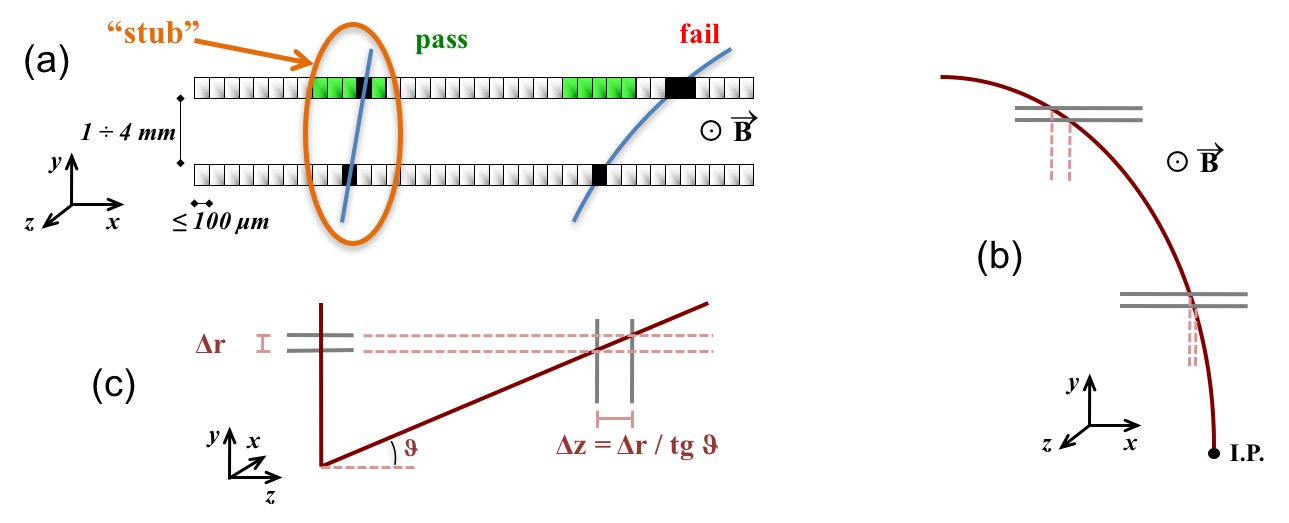
\includegraphics[width=5in]{figs/tk-upgrade/pTsketches.png}
% where an .eps filename suffix will be assumed under latex,
% and a .pdf suffix will be assumed for pdflatex; or what has been declared
% via \DeclareGraphicsExtensions.
\caption{Cluster matching in the $\pT$-modules proposed for the Outer Tracker~\cite{P2TrackerTDR} as described in the text; (a) demonstrates how correlating pairs of closely-spaced clusters between the two sensor layers allows for the discrimination of a track candidate's transverse momentum; (b) shows that if the sensor spacing remains unchanged, that the separation between the two clusters increases the further a module is away from the beam line; and (c) illustrates that the sensor spacing of modules in the endcap disks, which are perpendicular to the beam line, is required to be larger because of projective effects.
}
\label{fig:stubs}
\end{figure}

By correlating pairs of clusters on-detector that are consistent with a track with a transverse momentum of about 2\GeV or greater, an effective data rate reduction of approximately a factor of 10 is achieved before the resultant \emph{stubs} are transferred to the L-1 trigger~\cite{mpessimperf,2dptmoduleconcept}.

Two \pT modules are being developed for the Outer Tracker upgrade: 2S \emph{strip-strip} modules and PS \emph{pixel-strip} modules.
The 2S~modules, are designed to be used at radii $r>60$\cm from the beam line, where the hit occupancies are lower and each sensor has an active area of 0.05\cm~$\times$~9.14\cm.
Both 2S~module strip layers have a pitch of 90\mum in the transverse plane ($r$-$\varphi$) and a strip length of 5.03\cm along the direction of the beam axis, $z$.
Each PS~module sensor layer has an active area of 4.69\cm~$\times$~9.60\cm and will be used at radii in the range  $20<r<60$\cm where the occupancies are highest.
The upper PS~module layers consist of a silicon strip sensor and a silicon pixel sensor, both with a pitch of 100\mum in $r$-$\varphi$, and a strip length in $z$ of 2.35\cm for the strips and 1.47\mm for the pixels.
The finer granularity provided by the pixel layer affords better resolution along the $z$ axis, which is crucial for vertex identification in the high \PU environment of the HL-LHC.
Further details on the two \pT modules can be found in~\cite{CMS_Upgrade_TP,P2TrackerTDR}.

The current proposed layout of the Phase-II Outer Tracker, referred to as the \emph{tilted barrel} geometry, is depicted in the upper diagram in figure~\ref{fig:trackerlayout}, and a previous proposal, referred to as the \emph{flat barrel} geometry, is shown in the lower diagram~\cite{CMS_Upgrade_TP}.
Both plots illustrate the PS and 2S module positions in the six barrel layers and the five endcap disks on either side of the barrel, with only modules located at $|\eta| < 2.4$ being configured to send stub data off-detector.
The geometries are so named as they were inspired by whether or not the modules in the three innermost barrel layers are tilted so that their normals point towards the interaction region.
The advantages of the tilted geometry over the original flat barrel are that it not only improves stub-finding efficiency for tracks with large incident angles but also reduces the overall cost of the system~\cite{P2TrackerTDR}.
Due to the maturity of the preparations for the review between the three competing proposed track finder systems, discussed later in Section~\ref{subsec:TrackFinderReview}, at the time the tilted barrel geometry was adopted for the Phase-II Outer Tracker TDR it was decided to use the flat barrel geometry for results produced for the review.

\begin{figure}[tbp]
\centering
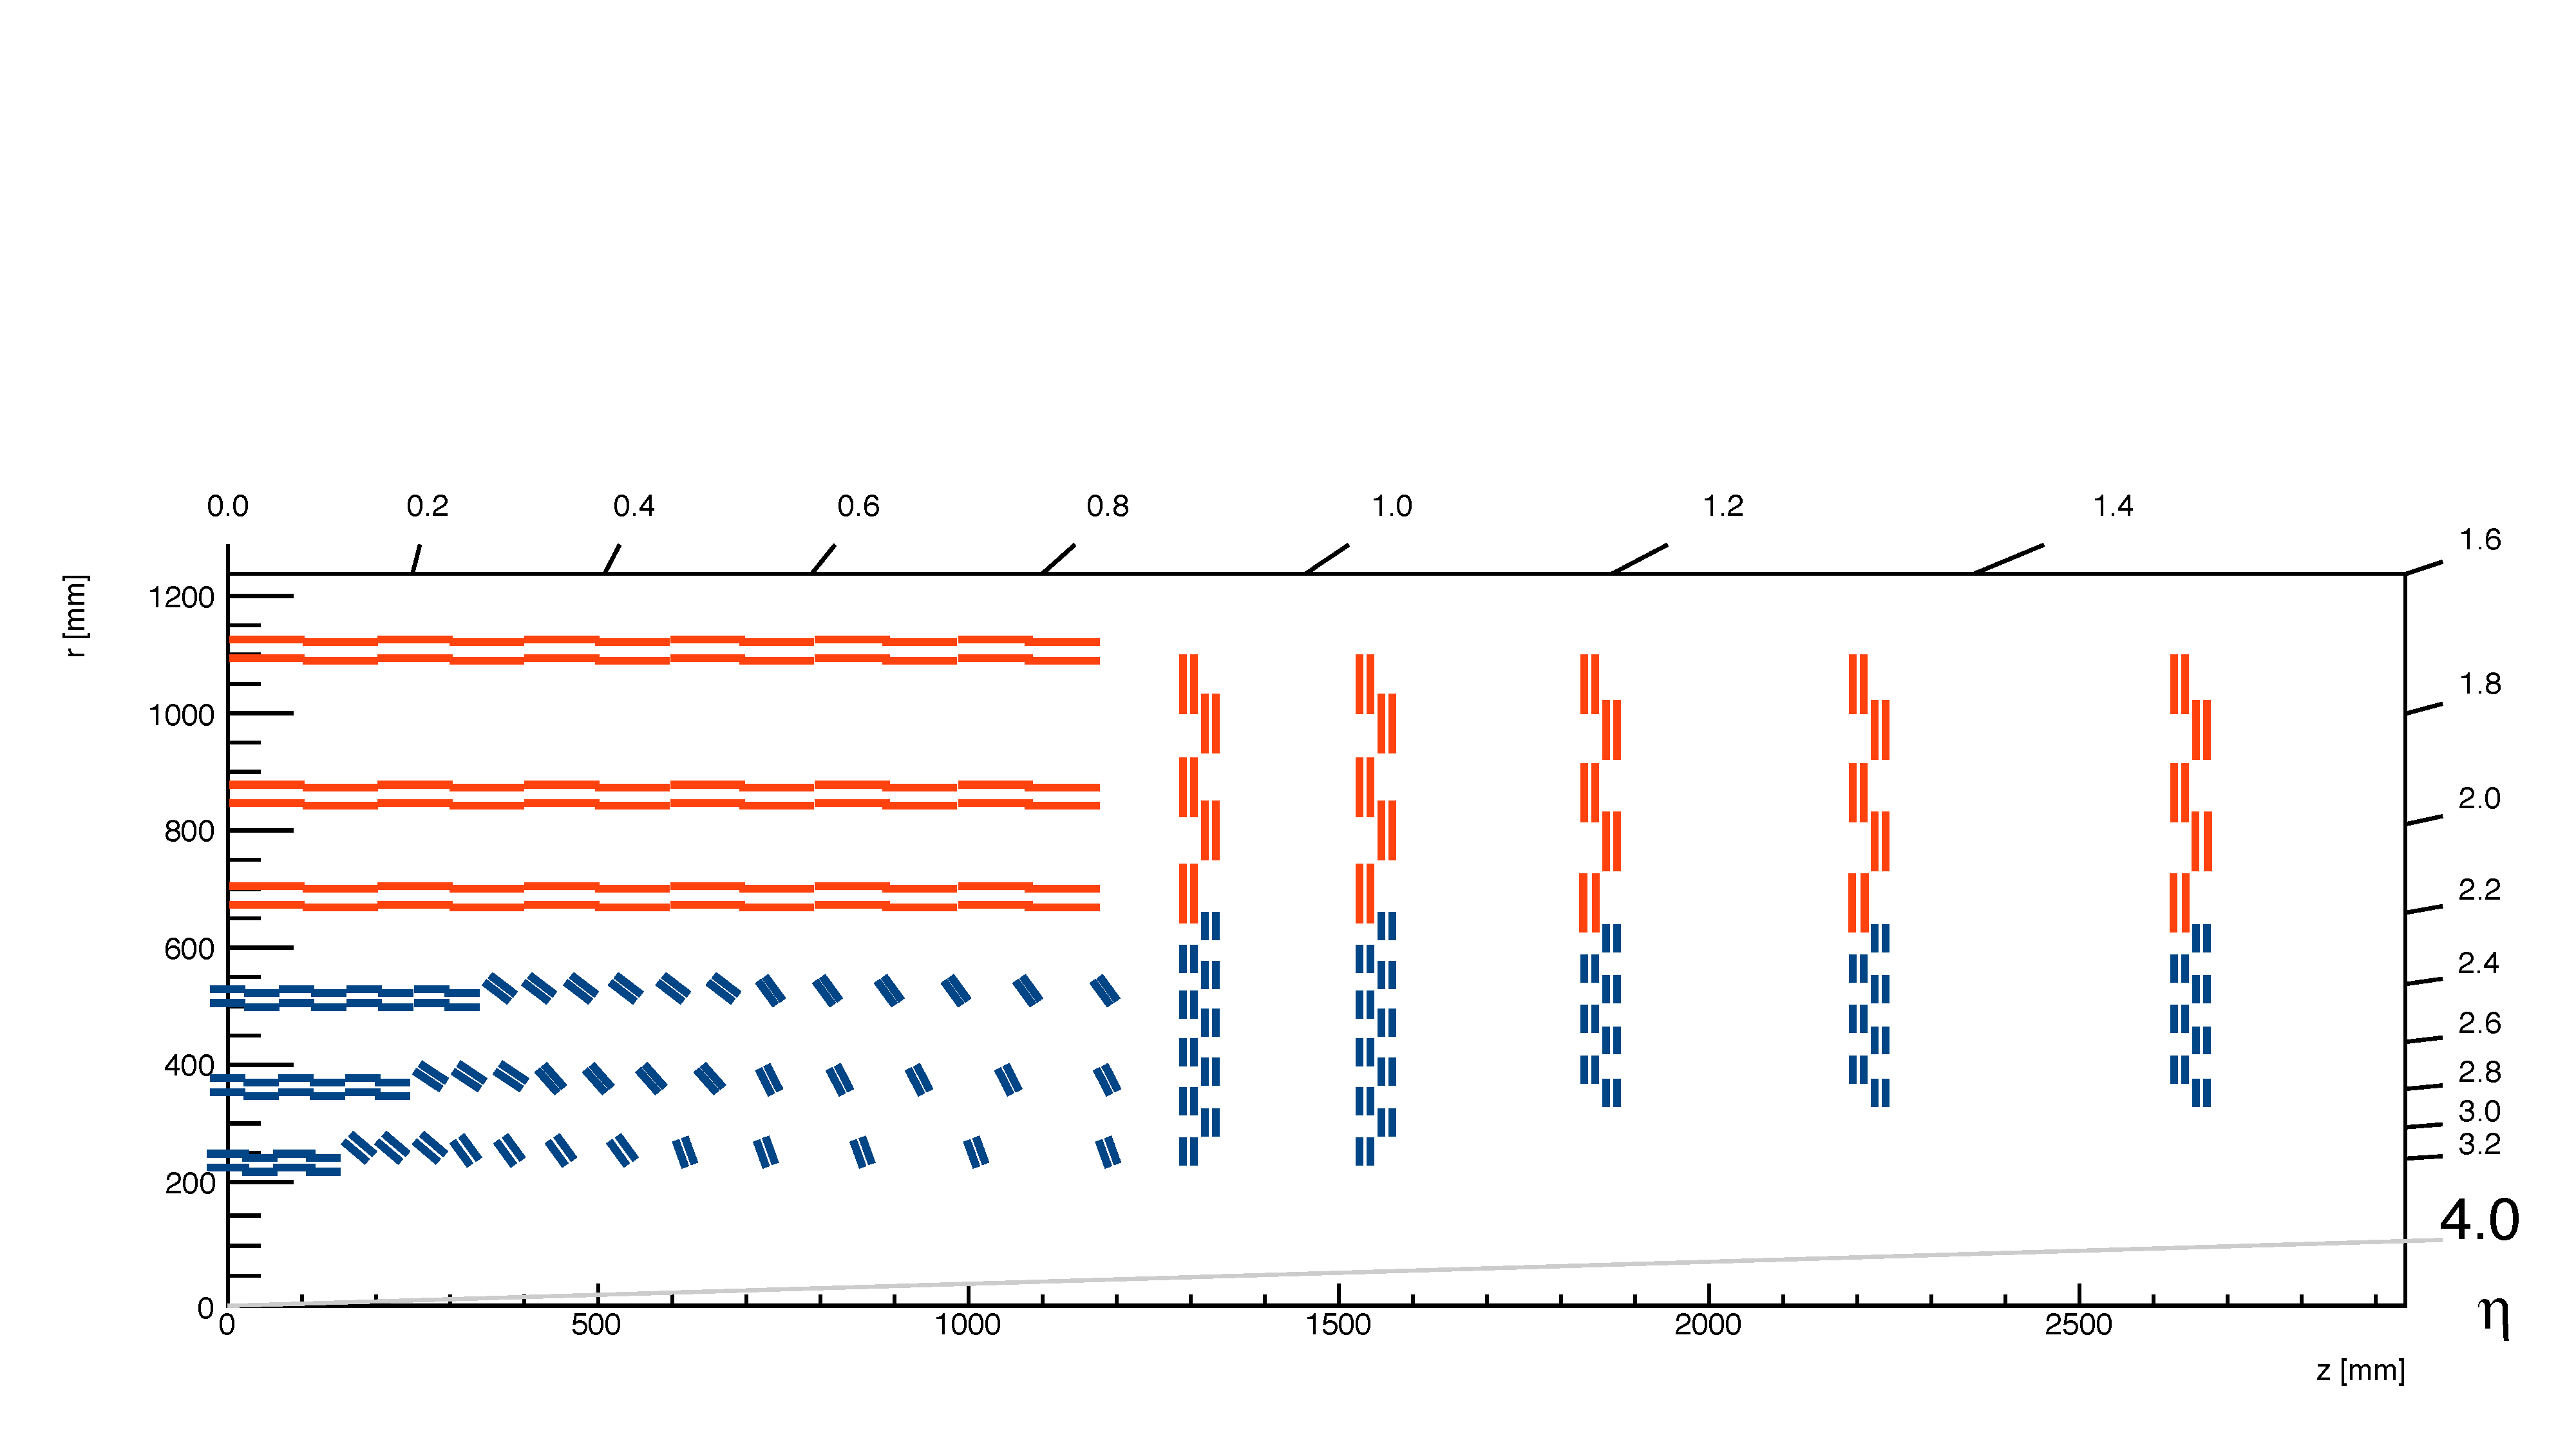
\includegraphics[width=0.8\textwidth,trim={1.1truecm 0truecm 1truecm 12truecm},clip]{figs/tk-upgrade/tiltedbarrelmap.pdf}
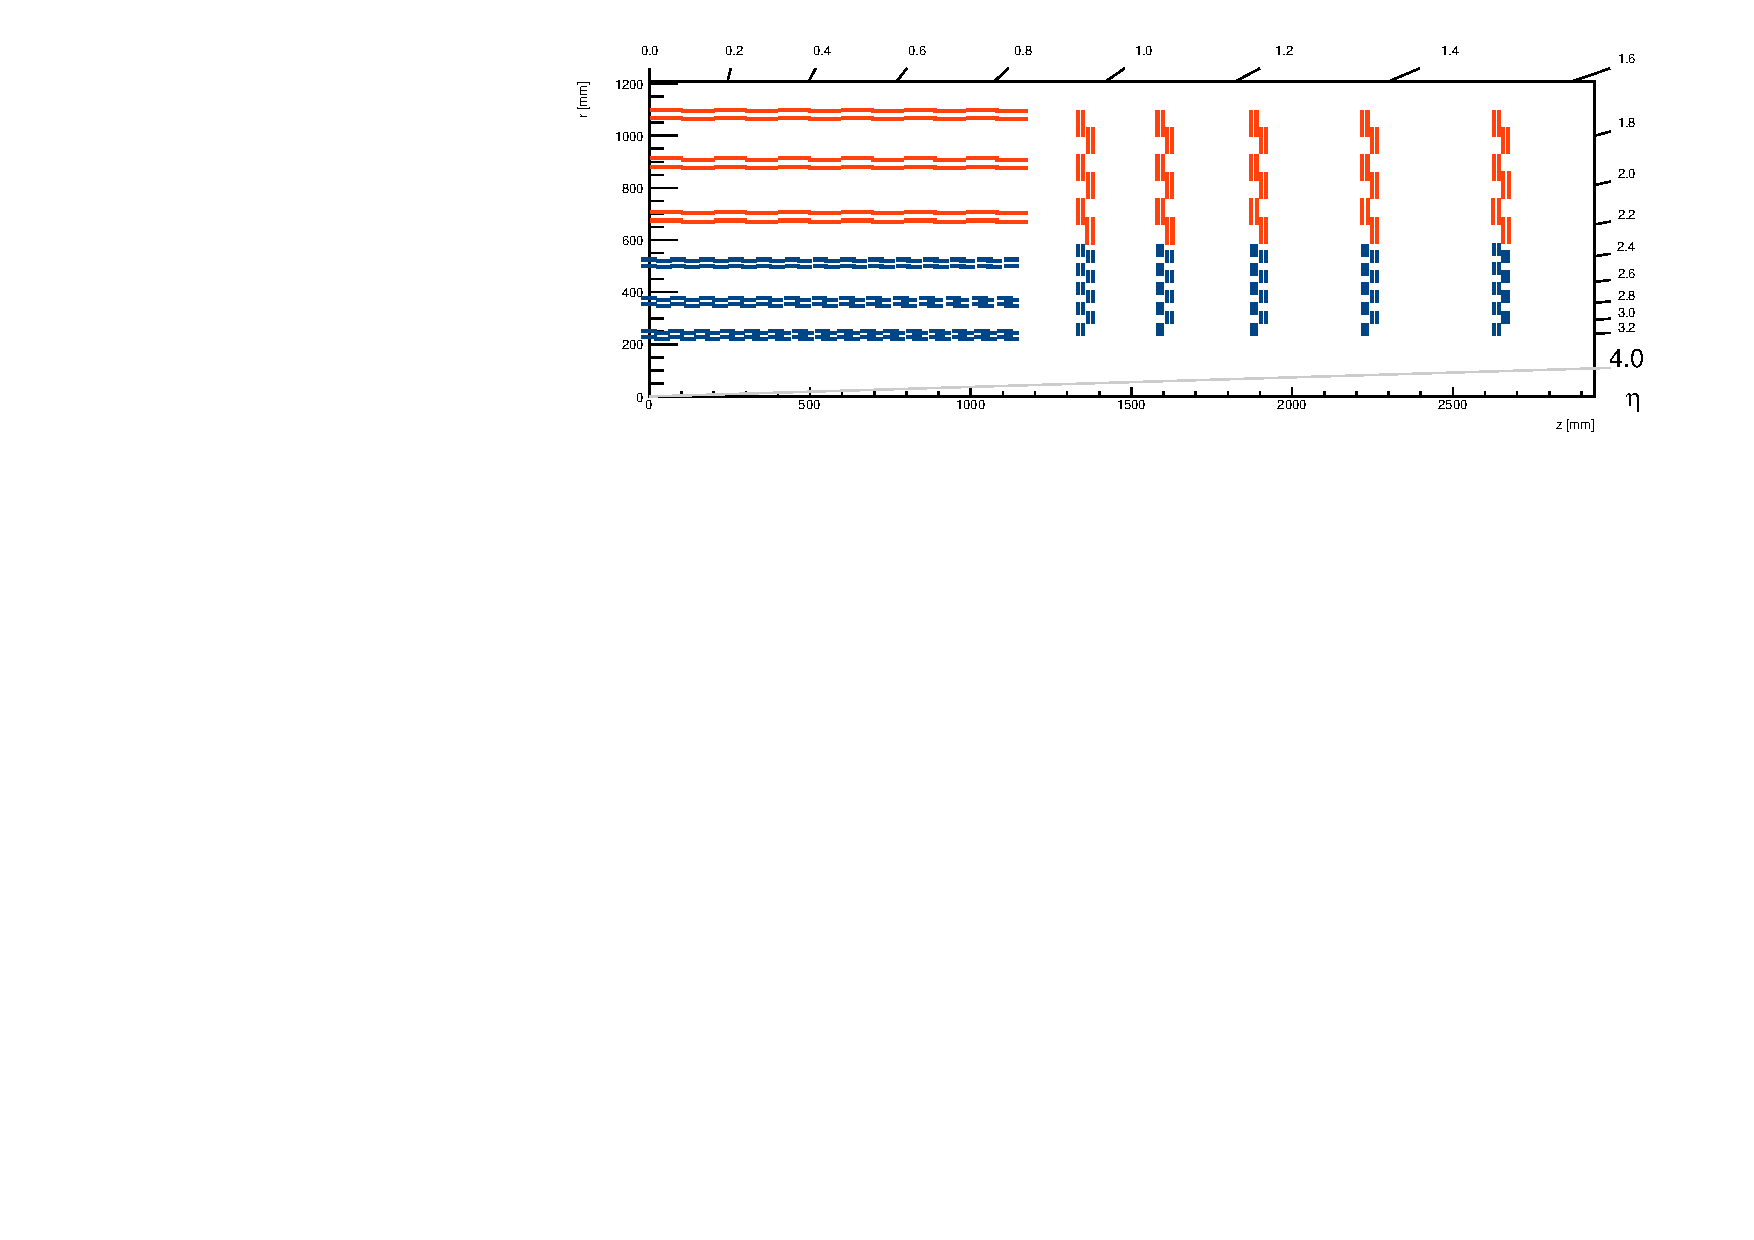
\includegraphics[width=0.8\textwidth,trim={0.7truecm 0truecm 1truecm 0truecm},clip]{figs/tk-upgrade/mersilayout.pdf}
\caption{One quadrant of the Phase-II Outer Tracker layout, showing the placement of the the PS (blue) and 2S (red) modules. The upper diagram shows the currently proposed \emph{tilted barrel} geometry~\cite{tiltedGeometry, P2TrackerTDR}, and the lower diagram shows an older proposal for the layout, known as the \emph{flat barrel} geometry \cite{CMS_Upgrade_TP}.}
\label{fig:trackerlayout}
\end{figure}

Out of the total L-1 latency of 12.5\mus, about $1\mus$ is required for generation, packaging and transmission of stubs from the tracker front-end (FE) electronics to the Data, Trigger and Control (DTC) system and approximately $4\mus$ is available for the reconstruction of tracks from data arriving at the DTC, as shown in figure~\ref{fig:dataFlow}.
The rest of the available latency is allocated for the correlation of tracks with trigger primitives from the calorimeters and muon systems ($3.5\mus$), the propagation of the L-1 decision to the front-end buffers ($1\mus$) and a safety margin ($3\mus$)~\cite{CMS_Upgrade_TP}.

The architecture of any Track Finder system proposed, which will take the pre-processed stubs as input and output fully reconstructed tracks for the L-1, will be constrained by the system's latency budget and how the detector is cabled to the DTC system.
The $4\mus$ latency constraint will limit the amount of processing that can be done for the finding and fitting of tracks and the choice of cabling scheme for the detector will determine how data is distributed and processed throughout the Track Finder system.

\begin{figure}[tb]
\centering
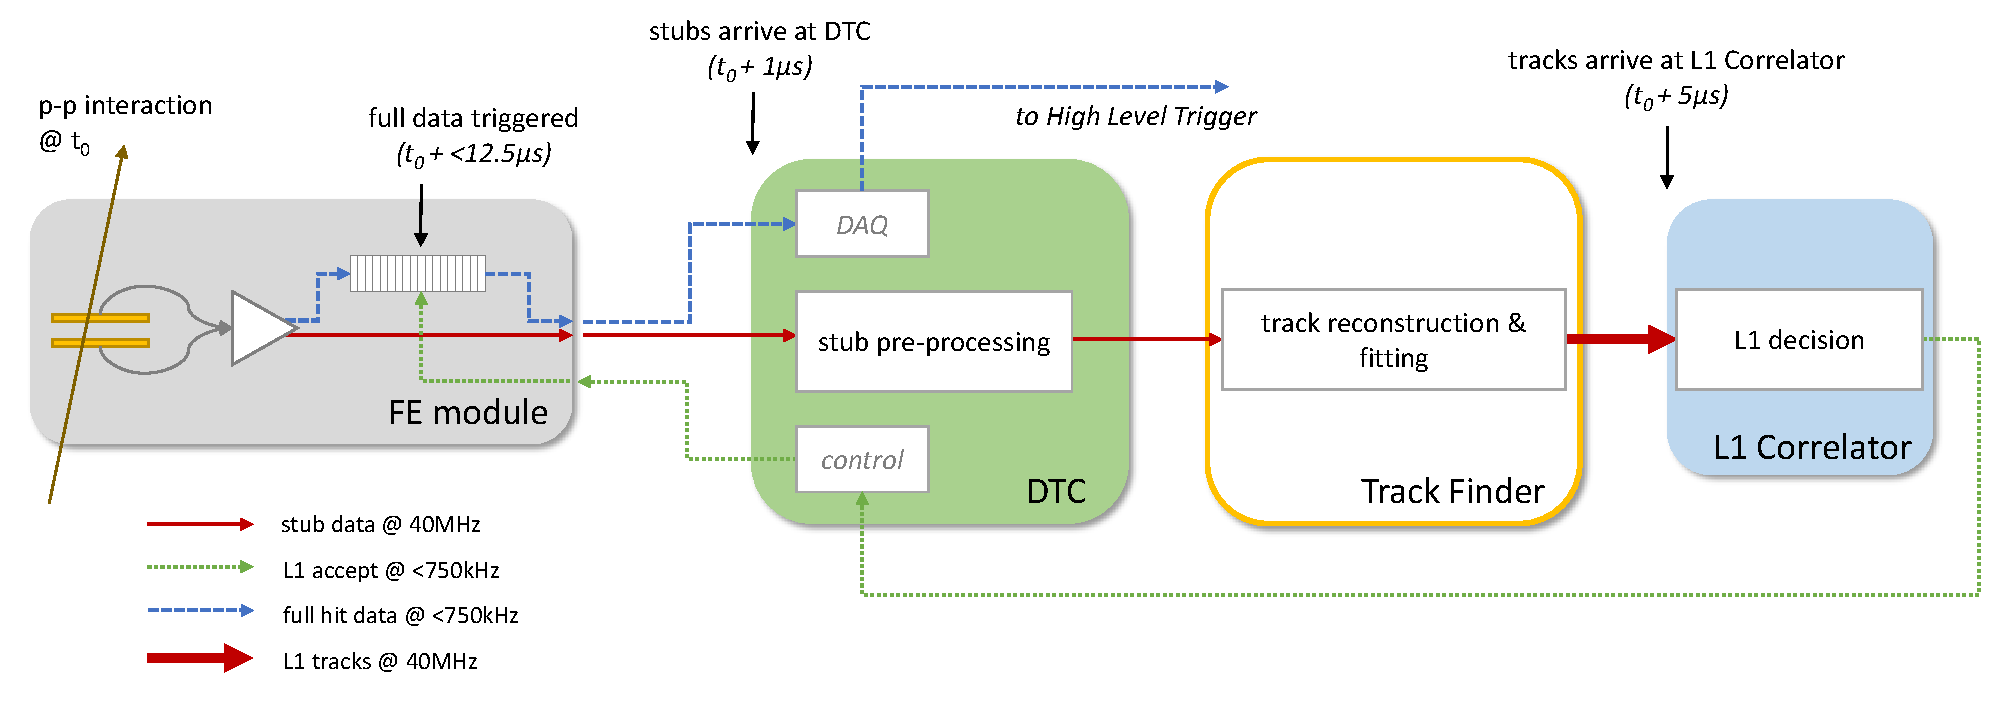
\includegraphics[width=\textwidth]{figs/tk-upgrade/dataflow.pdf}
% where an .eps filename suffix will be assumed under latex,
% and a .pdf suffix will be assumed for pdflatex; or what has been declared
% via \DeclareGraphicsExtensions.
\caption{Illustration of data flow and latency requirements starting from the \pt-modules and front-end (FE) electronicds and running through to the off-detector electronics dedicated to forming the L-1 trigger decision.}
\label{fig:dataFlow}
\end{figure}

\subsection{Level-1 Track Finding Proposals}\label{subsec:TrackFinderReview}

Three different L-1 track finders have been explored by the CMS Collaboration.
One uses Associative Memory (\emph{AM}) ASICs for track finding and FPGAs for track fitting, and the other two all-FPGA approaches, one using a fully Time-Multiplexed Track (\emph{TMT})finder which uses the Hough Transform to identify track candidates and one using a ``road search'' (\emph{tracklet}) algorithm to reconstruct tracks.

Hardware demonstrators for each of the three proposed L-1 track finder projects were constructed to prove the feasibility of each approach, which were reviewed in 2016.
As all of the work discussed in this chapter was on the FPGA-based \HT approach.
More detailed descriptions and results of both the AM and tracklet projects' approaches are not discussed here, but are given in earlier references~\cite{P2TrackerTDR,AM} and~\cite{P2TrackerTDR,tracklet} respectively.

As mentioned in Section~\ref{sec:tk-upgrade}, at the time of the review the flat barrel geometry described earlier was used for all the studies undertaken, as depicted in the lower diagram in figure~\ref{fig:trackerlayout}.
As such, unless stated otherwise, the results discussed below use the flat barrel geometry instead of the current tilted geometry.

\section{A Time-Multiplexed Track Finder }\label{sec:TMTT}
The Time-Multiplexed Track finder 

\subsection{The Track Finding Architecture}\label{subsec:TFA}
The proposed FPGA-based Hough Transform Track Finder is a scalable, flexible and redundant design based on a fully time-multiplexed architecture for implementation on commercially available FPGAs, as previously demonstrated by the Phase-I Calorimeter Trigger Upgrade~\cite{Tapper:2013yva} discussed in Section~\ref{paragraph:L-1}.
As discussed in Section~\ref{paragraph:L-1}, a time-multiplexed design has a number of advantages, including that only a single Track Finding Processor (TFP) is required to demonstrate the full system as each processor is identical in every respect.

Unlike the Phase-I Calorimeter Trigger, it is not feasible to process the entire output of the Phase-II Outer Tracker in a single processor for a given time slice because of the limits imposed by the input and total bandwidth a single FPGA-based processor can handle.
Therefore, as it was assumed at the time of the 2016 review that the DTC system would be arranged such that it forms octants~\footnote{These detector octants are not uniform as the geometry of the tracker does not have an exact eight-fold symmetry} (\ie 45 degree $\varphi$-sectors, referred to as \emph {detector octants}) in the tracker, the baseline system proposed was divided into \emph{processor octants} that were offset from the detector octants by $\approx 22.5$ degrees in $\phi$, in order to handle data duplication across hardware boundaries.
This baseline system architecture, illustrated in figure~\ref{fig:tmttarch}, uses two neighbouring DTCs to time-multiplex and duplicate stub data across processing octant boundaries before each DTC transmits 50\% of its data to one TFP and 50\% to the neighbouring TFP.
Based on current electronics and the high speed links available, the data requires 18 TFPs per processing octant (one for each time slice, resulting in a full system requiring 144 TFPs).

\begin{figure}[t]
\centering
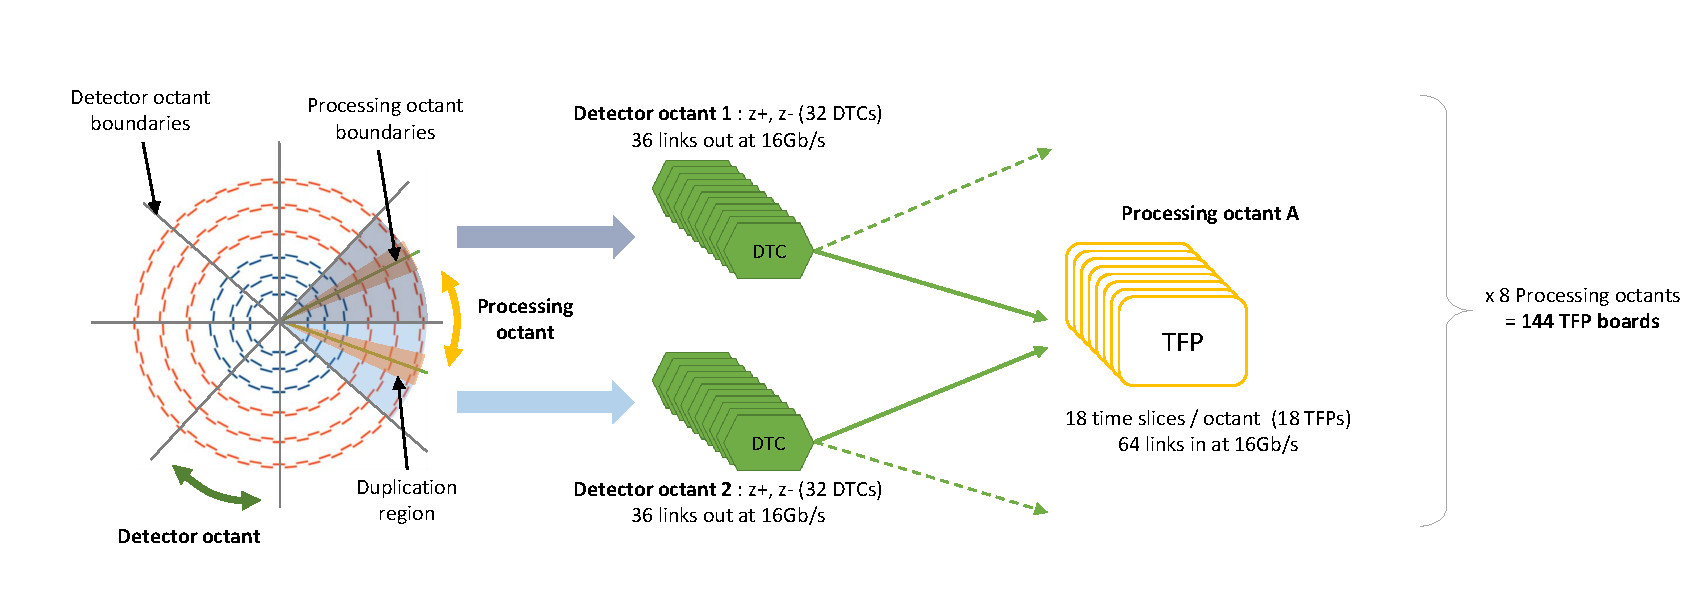
\includegraphics[width=1.00\textwidth]{figs/tk-upgrade/tmttarch.pdf}
\caption{An illusratation of the baseline system architecture described in the text, demonstrating how two neighbouring DTCs time-multiplex and duplicate stub data across processing octants and how it transmits the processed data to two neighbouring TFPs~\cite{TMTT_JINST}}
\label{fig:tmttarch}
\end{figure}

A hardware demonstrator of the baseline system consisting of five Imperial Master Processor Virtex-7 (MP7) cards~\cite{mp7ref}, capable of processing one phi-octant of the tracker with a time-multiplexing factor of 36, was used to validate the feasibility of the proposed full system using hardware available at the time of the 2016 review.
All of the results achieved, and a complete description of the system, are given in~\cite{TMTT_JINST}.

\subsection{The Track Finding Processor}\label{subsec:TFP}
The Track Finding Processor shown in figure~\ref{fig:TFP} consists of four self-contained components:
\begin{itemize}
\item {\bf Geometric Processor (GP)} Responsible for pre-processing the stubs from the DTC.
\item {\bf Hough Transform (HT)} A highly parallelised initial coarse track finding.
\item {\bf Kalman Filter (KF)} Removes incorrectly associated stubs from a track, precisely fits helix parameters and removes fake tracks.
\item {\bf Duplicate Removal (DR)} A final pass filter that uses the precise fit information to remove duplicate tracks generated by the \HT.
\end{itemize}

Each of these components is described in more detail below.

\begin{figure}[!h]
\centering
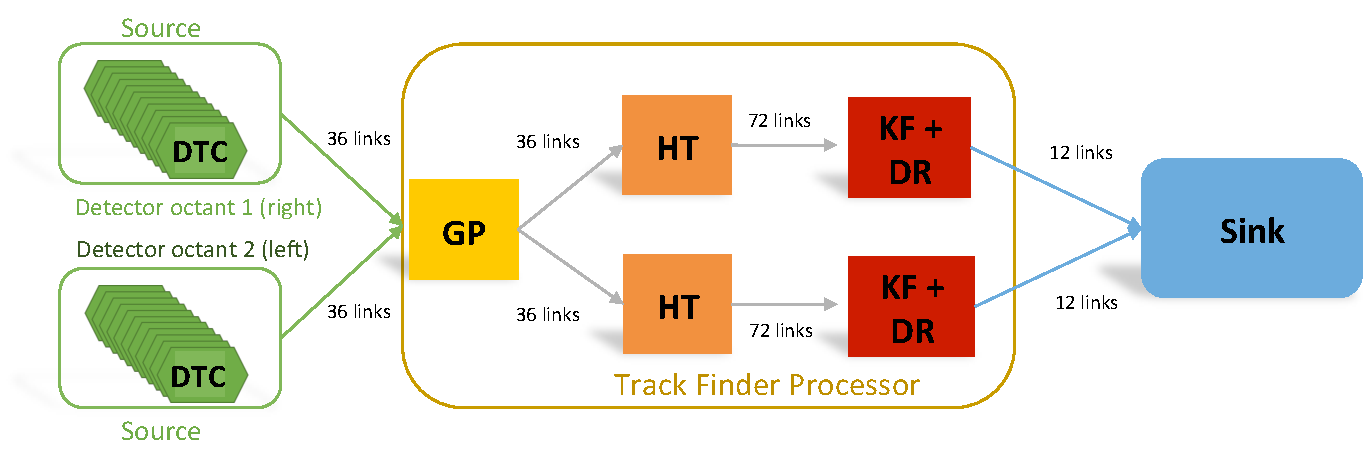
\includegraphics[width=0.78\textwidth]{figs/tk-upgrade/demoslice1.pdf}
% where an .eps filename suffix will be assumed under latex,
% and a .pdf suffix will be assumed for pdflatex; or what has been declared
% via \DeclareGraphicsExtensions.
\caption{The four self-contained logical components of the Track Finding Processor, where each box (block) in the diagram represents a single FPGA. The two FPGAs for the two detector octant sources and the sink FPGA and the optical links between all components are also shown.}
\label{fig:TFP}
\end{figure}

\subsubsection{Geometric Processor}\label{subsubsec:GP}
Each GP performs two tasks: the conversion of the 48-bit DTC stubs into a 64-bit format extended format that is used to reduce the HT processing load and assignment of the stubs in each sector into a subsector. 
Each sector is composed of 2 sub-sectors in $\phi$ and 18 in $\eta$.

This division of the processing octants simplifies the task of the downstream logic, allowing the track finding to be carried out independently and in parallel within each sub-sector. 
The chosen $\eta$ binning is sufficiently fine to ensure that any track found by the \rphi HT is consistent with a straight line in the \rz plane, despite the fact the \HT itself only searches for tracks in the \rphi plane, thus rejecting incompatible track candidates.

Stubs that are compatible with more than one sub-sector, usually due to track curvature in $\phi$, are duplicated. 

Stubs are assigned to sub-sectors occurs in a three stage process:
\begin{itemize}
\item A rough $\eta$ sorting into six bins;
\item A subsequent fine $\eta$ sorting into three bins and;
\item A $\phi$ sorting into two bins. 
\end{itemize}

Each of the TFP's logic blocks shown in figure~\ref{fig:TFP} has been designed to be highly reconfigurable and can easily be adapted to any alternative sub-sector definition.

\subsubsection{Hough Transform}
The Hough Transform algorithm is a widely used means of detecting geometric features in digital image processing \cite{HT}.

%%% GENERAL INTRO

 and is used by the TFP to find charged particles with $\pT > 3\GeV$ in the \rphi plane. 

Within the tracking volume, permeated by a homogeneous 3.8T magnetic field ($B$), a track  with a radius of curvature ($R$) can be described as a function of its \pT and charge $q$:

\begin{equation}
R = \frac{\pt}{0.003\,qB} \;
\label{eq:R}
\end{equation}

Assuming, to first order, that $R$ is constant, by neglecting energy losses such as through multiple scattering, and that only primary tracks from or near the primary interaction point are considered (other such tracks are not typically relevant to the L-1 trigger), a stub with coordinates ($r$,$\varphi$) is related to $R$ by:

\begin{equation}
\frac r{2\,R} = \sin\left(\varphi-\phi\right) \;
\label{eq:stub_R}
\end{equation}

where $\phi$ is the angle of the track in the transverse plane at the origin \cite{markthesis}. 
For large \pT ($> 3\GeV$) and thus large $R$, the small angle approximation can be used. Combining Equations~(\ref{eq:R}) and (~\ref{eq:stub_R}), one produces the key formula showing the transformation from stub positions to straight lines in the track parameter plane (Hough-space):

\begin{equation}
\phi = \varphi - \frac{0.0015\,qB}{\pt}\cdot r \;
\label{eq:localHT}
\end{equation}

The point of intersection of these lines in Hough-space would therefore correspond to a circle in the \rphi plane which is consistent with the primary interaction point and all stubs involved.
As the line gradients in Hough-space is given by the radius of the stubs, they will always be positive, the stub radius is transformed to $r_{58} = r - 58cm$ in order to utilise a larger phase space, which leads to fewer \textit{fake} (in that the found track does not match to a simulated particle) and duplicated tracks.

Given that $R$ for the lowest \pT track (3\GeV) to be considered is greater than the outer radius of the tracking detector ($r$ = 1.2m), all relevant particles are expected to traverse through at least six barrel layers or endcap disks. 
The threshold for the identification of a track candidate however, is set at a minimum of five detector layers or disks in order to allow for detector or readout inefficiencies. 
This threshold can be further reduced to four layers to account for the reduced geometric coverage between $0.89 < \eta < 1.16$ or for dead detector layers or disks.

A more detailed description of the firmware implementation of the \HT for the demonstrator system is discussed in~\cite{TMTT_JINST,IEEE}.

\subsubsection{Kalman Filter}\label{subsubsec:KF}
\editComment{More detail - including on the covariance matrix ...}
The coarse \rphi helix parameters that are output by the \HT are used as the initial variables for track finding, with the segment assignment also providing a good seed value.
Given that in simulation over half the track candidates from by the HT are considered to be \textit{fake} or contain at least one stub associated with another particle, a Kalman Filter is used to both remove these incorrect stubs and reject fake tracks. 

In addition to the advantages of the Kalman filter for track reconstruction discussed by Fr{\"u}hwirth in \cite{Fruhwirth:1987fm}, the algorithm has several aspects making it suitable for FPGA implementation compared to global track fitting methods, namely the matrices:

\begin{itemize}
\item {are small.}
\item {are sized independently of the number of measurements.}
\item {only involve the inversion of a small matrix.}
\end{itemize}

The initial estimates, or \textit{state}, of the track parameters and their uncertainties, $\chi^2$ value and other status information are updated by the KF iteratively applying stubs to update the state following the Kalman formalism, decreasing the uncertainty in the state. 
Each update of the state can be filtered on number of configurable criteria, including \pT, $\chi^2$, and the minimum number of stubs from PS modules, and can take into account and skip missing missing layers due to missing or incorrect stubs.
In the event multiple stubs are found on the same layer, each can be propagated with up to the four best states being kept and presented to a final state selector, with preference given to states with the fewest missing layers and the smallest $\chi^2$.
The final fit is always performed after a fixed period of time, so consequently there is no truncation in the traditional sense as all candidates will be read out, although events such as dense jets with many candidates and stubs per candidate will only be partially filtered.

A greater in-depth discussion of the mathematics and implementation of online track reconstruction using Kalman Filters on FPGAs in~\cite{SSummers}.

\subsubsection{Duplicate Removal}
Following the \KF, over half of the track candidates are unwanted duplicate tracks created by the HT.
Instead of comparing pairs of tracks to see if they are the same, a more elegant and subtle DR algorithm is used which takes into account how the \HT produces these duplicate tracks.
This approach is illustrated in figure~\ref{fig:DR}, where five stubs, which correspond to the blue lines in Hough Space, produce candidates in the green and two yellow cells.
The coarse track finding performed by the \HT 

however, as all three candidates contain the same stubs, they will be fitted with identical helix parameters in the same cell (the yellow cell) regardless of the original HT cell.


The DR algorithm accepts only tracks whose fitted parameters are consistent with the \HT cell in which they were initially found. 
There is however, a small subtlety, given that the algorithm eliminates unique tracks whose fitted parameters were not consistent, which results in the loss of a few percent of efficiency. 
By performing a second pass through the rejected tracks, tracks which have fitted parameters that do not correspond to the HT cell of a track from the first pass are probably not duplicates, and so they are recovered.

\begin{figure}[!h]
\centering
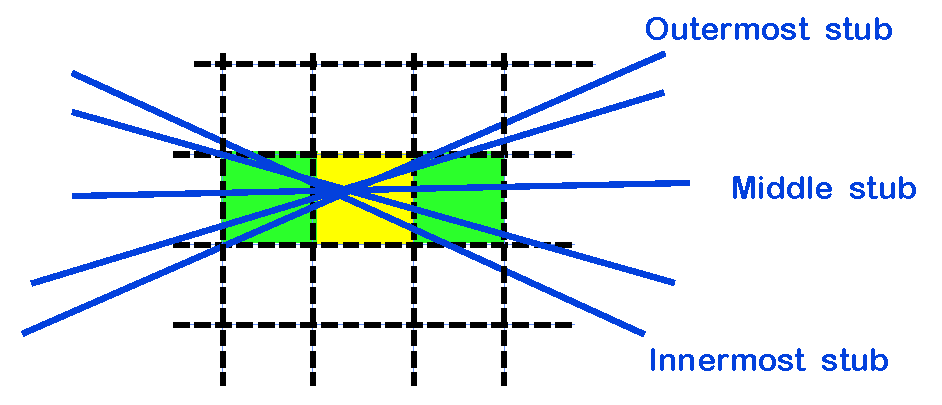
\includegraphics[width=0.80\textwidth]{figs/tk-upgrade/A50_algo.pdf}
% where an .eps filename suffix will be assumed under latex,
% and a .pdf suffix will be assumed for pdflatex; or what has been declared
% via \DeclareGraphicsExtensions.
\caption{Illustration of how duplicates are formed by the \rphi \HT.}
\label{fig:DR}
\end{figure}

A more detailed description of the firmware implementation of the \DR for the demonstrator system is discussed in~\cite{TMTT_JINST}.

\section{Simulation Studies}\label{sec:TmttSimStudies}
This section presents a number of simulation studies which were undertaken as part of the development of the \emph{TMT} finder demonstrator system both before and following the 2016 review.
All of the results discussed use a common set of definitions, as defined in Section~\ref{subsec:helixParameter}, and the track fitters discussed use digitised output from the \HT.

\subsection{Definitions}\label{subsec:helixParameter}
A number of parameters and metrics are used throughout this chapter to describe tracks and how well the track fitters have reconstructed them.
They are defined as below.

\subsubsection{Helix Parameters}
The helical trajectory of a charged particle at the impact point is described by five helix parameters.
In the CMS these parameters are defined as:

\begin{itemize}
\item $\mathbf{p_{T}}$ - the transverse momentum of the track;
\item $\mathbf{\phi_{0}}$ - the track angle in the transverse plane;
\item $\mathbf{z_{0}}$ - the \emph{longitudinal} impact parameter, \ie the distance in z from the point of closest approach to the interaction point;
\item $\mathbf{\cot(\theta)}$ - the cotangent of the \emph{dip} (polar) angle, related to $\eta$ by $\cot(\theta) = \sinh (\eta)^{-1}$;
\item $\mathbf{d_{0}}$ - the \emph{transverse} impact parameter, \ie the distance of the track vertex from the interaction point in the $x-y$ plane. 
\end{itemize}

As the \HT and track fitting algorithms discussed all assume that all tracks originate at the interaction point, $d_{0}$ is not given in the results below as it is fixed to zero.

\subsubsection{Reconstructed Tracks}
The common definitions of track reconstruction efficiency~\cite{TMTT_JINST} used for the three proposed L-1 Track Finder systems are used for the results presented in this chapter:

\begin{itemize}
\item The reconstruction efficiency is measured relative to all generated charged particles from the primary interaction that produce stubs in at least four layers of the tracker which satisfies the following conditions: $\pT > 3\GeV$, $|\eta| < 2.4$, $|z_{0}| < 30\cm$ and $d_{xy} < 1\cm$, where $d_{xy}$ is the distance in the $x-y$ plane from the point of closest approach to the interaction point.
\item A track is a defined as being correctly reconstructed or \emph{matched} if the reconstructed track has stubs associated to the particle in at least four tracker layers. Tracks which fail this matching criteria are known either as \emph{unmatched} or \emph{fake} tracks.
\item If the reconstruction of a charged particle produces more than one track, these additional tracks are considered to be \emph{duplicates}.
\item If all a reconstructed track's stubs originated from the same particle, the track is defined as being \emph{perfectly} reconstructed. 
\end{itemize}

This stricter definition of \emph{perfect} track reconstruction efficiency is typically used in quoting results from the entire chain (\ie all four components of the TFP discussed in Section~\ref{subsec:TFP}).
Otherwise, the nominal definition of track reconstruction efficiency is used as the presence of stubs incorrectly associated with a track is to be expected if only part of the TFP chain has been run.
Where appropriate, the results for both definitions are given.


\subsection{Linearised $\chi^{2}$ Track Fitter}\label{subsec:chi2}

Three different track fitting algorithms were explored for the track fitter to be used for the 2016 hardware demonstrator review: a Kalman Filter, a Linear Regression (LR) algorithm and a linearised $\chi^{2}$ track fit.

The Kalman Filter was selected for the 2016 review as it provided the best and an identical track reconstruction efficiency and the highest fake track rejection rate.

The Linear Regression (LR) algorithm~\cite{TMTT_FLP} was developed as an alternative to the KF and exploits the fact that sufficiently high \pT tracks should form a straight line in the \emph{\rphi} and \emph{r-z} planes to perform independent fits in each plane.
While it has

The studies of the linearised $\chi^{2}$ track fit were initially motivated by the \emph{TMT} project anticipating potential time and resource pressures in developing all the components of a complete track finder system that could be implemented in hardware due to the project being formed significantly after the other two L-1 track finder projects.

Following discussions with both the \emph{tracklet} and \emph{AM} projects, it was decided that the use of a linearised $\chi^{2}$ fit based on the one proposed by the \emph{tracklet} project would be investigated.
The general form of the $\chi^{2}$ fit and the derivation of the track derivatives required by the algorithm were provided in a private communication~\cite{CMS_DN-14-043} and were used to produce a \emph{TMT} implementation of the algorithm.

A linearised $\chi^{2}$ fit calculates improved helix parameters for the track candidate by determining the  residuals between the stubs and the seeded track that minimise the $\chi^{2}$ of the fit.

The general form of the $\chi^{2}$ fit describing how these hit residuals are used to obtain a fit of a track's helix parameters is detailed in Section~\ref{subsubsec:chi2maths}.
A discussion of the development and outcomes of the software implementation of the fitting algorithm are given in Sections~\ref{subsubsec:chi2software} and~\ref{subsubsec:chi2outlook}.


The calculation of the track derivatives for the barrel layer hits and endcap disk hits used by the algorithm, included a correction factor for $\phi$ in the outer disks to account for the fact that these modules do not point directly towards the interaction point, which is described in Appendix~\ref{app:chi2}.

All the results presented here involve the use of a \emph{Seed Filter} (SF) stage that was run following the \HT stage for both the Linear Regression and Linearised $\chi^{2}$ fitting algorithms.
This process removes stubs in a \HT cell that are inconsistent with a straight line in the \emph{r-z} plane and filters out both fake tracks and stubs incorrectly assigned to tracks (also referred to as \emph{fake} stubs).

\subsubsection{General Form of a $\chi^{2}$ Fit}\label{subsubsec:chi2maths}
For the general form of a $\chi^{2}$ fit for a track, $f$, described by its helix parameters, $\overrightarrow{h}$, and 
the position of its $i$ hits (\ie stubs) given at $s_{i}$, we initially linearly expand the projection of the track, $f_{i}$, around the estimate of the helix parameters $\overline{h}$:

\begin{equation}
f_{i}(\overrightarrow{h} ) = f_{i}(\overrightarrow{h} + \delta \overrightarrow{h}) \;
                           = f_{i}(\overline{h} + \delta \overrightarrow{h} \frac{\partial f_{i}}{\partial \overrightarrow{h}} + \mathcal{O}(\delta \overrightarrow{h}^{2}) \;
\label{eq:chi1}
\end{equation}

The $\chi^{2}$ of such a track is expressed as:

\begin{equation}
\begin{split}
\chi^{2} &= \sum_{ij} \big(f_{i}(\overrightarrow{h}) - s_{i} \big) V^{-1}_{ij}  \big(f_{j}(\overrightarrow{h}) - s_{j} \big)  \\
         &= \sum_{ij} \big( f_{i}(\overline{h})  - s_{i} + \delta \overrightarrow{h} \frac{\partial f_{i}}{\partial \overrightarrow{h}} \big) V^{-1}_{ij}  \big( f_{j}(\overline{h})  - s_{j} + \delta \overrightarrow{h} \frac{\partial f_{j}}{\partial \overrightarrow{h}} \big)  \\
         &= \sum_{ij} \big( \delta f_{i} + \delta \overrightarrow{h} \frac{\partial f_{i}}{\partial \overrightarrow{h}} \big) V^{-1}_{ij}  \big( \delta f_{j} + \delta \overrightarrow{h} \frac{\partial f_{j}}{\partial \overrightarrow{h}} \big)
\end{split}
\label{eq:chi2}
\end{equation}

where $\delta f_{i} \equiv f_{i}(\overline{h}) - s_{i}$ are the residuals between the expected position of the track (given by the seed helix parameters) and the position of the track given by the stub, and $V^{-1}_{ij} = diag(\sigma^{2}_{ii})$ is the variance matrix that describes the uncertainty associated with the measurement of the stubs.

By minimising the $\chi^{2}$, $\delta h$ can be determined:

\begin{equation}
0 = \frac{\partial \chi^{2}}{\partial \delta \overrightarrow{h_{k}}} = \sum_{ij} \frac{\partial f_{i}}{\partial \delta \overrightarrow{h_{k}}} V^{-1}_{ij} ( \delta f_{j} + \delta \overrightarrow{h} \frac{\partial f_{j}}{\partial \overrightarrow{h}} ) + \sum_{ij}	( \delta f_{i} + \delta \overrightarrow{h} \frac{\partial f_{i}}{\partial \overrightarrow{h}} ) V^{-1}_{ij} \frac{\partial f_{j}}{\partial \delta \overrightarrow{h_{k}}}  \;
\label{eq:chi3}
\end{equation}

By defining the matrices $D_{ij} = \frac{\partial f_{i}}{\partial h_{k}}$ and $M = D^{T} V^{-1} D$, Equation~(\ref{eq:chi3}) can be rewritten and solved for $\delta h$:

\begin{equation}
0 = D^{T} V^{-1} \delta f + M \delta h \Rightarrow \delta h = - M^{-1} D^{T} \delta f \;
\label{eq:chi4}
\end{equation}

Therefore Equation~(\ref{eq:chi4}) provides a simple linear form for how the track helix parameters should be updated for a set of residuals with respect to the seed track candidate.

Similarly the $\chi^{2}$ of the fit can also be expressed in a linear form:

\begin{equation}
\begin{split}
\chi^{2} &= (\delta f + D \delta h)^{T}(\delta f + D \delta h) \\
         &= (\delta f - DM^{-1}D^{T}\delta f)^{T} (\delta f - DM^{-1}D^{T}\delta f) \\
         &= \delta f^{T} (1- DM^{-1}D^{T}) (1- DM^{-1}D^{T}) \delta f \\
         &= \delta f^{T} (1- DM^{-1}D^{T}) \delta f \\
         &= \delta f^{T} \delta f - \delta f^{T} DM^{-1}D^{T} \delta f \\
         &= \chi^{2}_{seed} + \delta f^{T} D \delta \overrightarrow{h} 
\end{split}
\label{eq:chi5}
\end{equation}

As the linear forms of Equations~(\ref{eq:chi4}) and~(\ref{eq:chi5}) consist of repeated addition and multiplication operations of the matrices involved, they are naturally suitable for implementation on an FPGA.

While FPGAs can easily perform such operations, potential complications arise when considering the calculation of the track derivatives that form the elements of $D$ which would not be trivial given the presence of a large number divisions and trigonometric functions for the endcaps' derivatives.
Therefore, any implementation in firmware for an FPGA will require the use of lookup tables containing the precomputed values of the derivatives in order to quickly update a track's helix parameters without exceeding latency budgets.

\subsubsection{Software Results}\label{subsubsec:chi2software}
From equations~(\ref{eq:chi4}) and~(\ref{eq:chi5}) and the track derivatives derived in Appendix~\ref{app:chi2}, a software implementation of the linearised $\chi^{2}$ track fit algorithm was developed.
Initially this implementation used exact floating point mathematics in order to validate the algorithm, before a version using approximated expressions of the track derivatives was developed.
The motivation behind this was to reduce the number of variables that the matrix of derivatives would depend on in order to simplify (and reduce resources required for) any future tabulation of the matrix.

\begin{table}[htbp]
\topcaption {Track finding performance on simulated \ttbar events at a <PU> of 200, after the \HT and the full chain for  both the exact floating point and approximated calculations of the track derivatives used by the $\chi^{2}$ track fit.
The track finding efficiencies following each stage are given using the efficiency definitions given in Section~\ref{subsec:helixParameter}, along with the mean number of tracks and the fraction of those tracks which are either fake or duplicate tracks.
\editComment{Fix table size}
}

\label{tab:chi2-exactVsApprox}
 \centering
 \resizebox{\textwidth}{!}{
% This right-aligns numbers in column, but centers them under column title.
 \begin{tabular}{cccccc}
   \hline
   \bf{Stage} & \bf{Efficiency [\%]} & \bf{``Perfect'' Efficiency [\%]} & \bf{Mean \# of tracks} & \\bf{Fakes [\%]} & \bf{Duplicates [\%]}  \\
        \hline
   HT &  97.0 & 43.1 & 351.2 & 43.9 & 37.0 \\  
   \hline
   $\chi^{2}$+DR & 95.0 & 85.8 & 86.4 & 15.7 & 9.5 \\
   (floating point) & & & & & \\
   \hline
   $\chi^{2}$+DR & 94.9 & 85.6 & 87.4 & 15.5 & 10.9 \\  
   (approximated) & & & & & \\   
%   \hline
%   KF+DR & 94.1 & 94.1 & 82.1 & 21.1 & 4.5 \\
   \hline
   
 \end{tabular}}
\end{table}

Table~\ref{tab:chi2-exactVsApprox} shows how the tracking performance compares between the floating point maths and ``approximated'' maths versions of the algorithm compare against each other and from the raw track finding output from the \HT.
It can be seen that whilst the \HT finds tracks with high efficiency, over half have at least one incorrectly associated stub and a significant number of the tracks found are fake or duplicated tracks.
Both floating point and approximated maths implementations give comparable results, indicating that the approximations made are acceptable.
The $\chi^{2}$ track fit increases the purity of the reconstructed tracks by a factor of two and eliminates the majority of the fake tracks, whilst the \DR algorithm removes the majority of the duplicates.



\begin{figure}[htb]
\centering
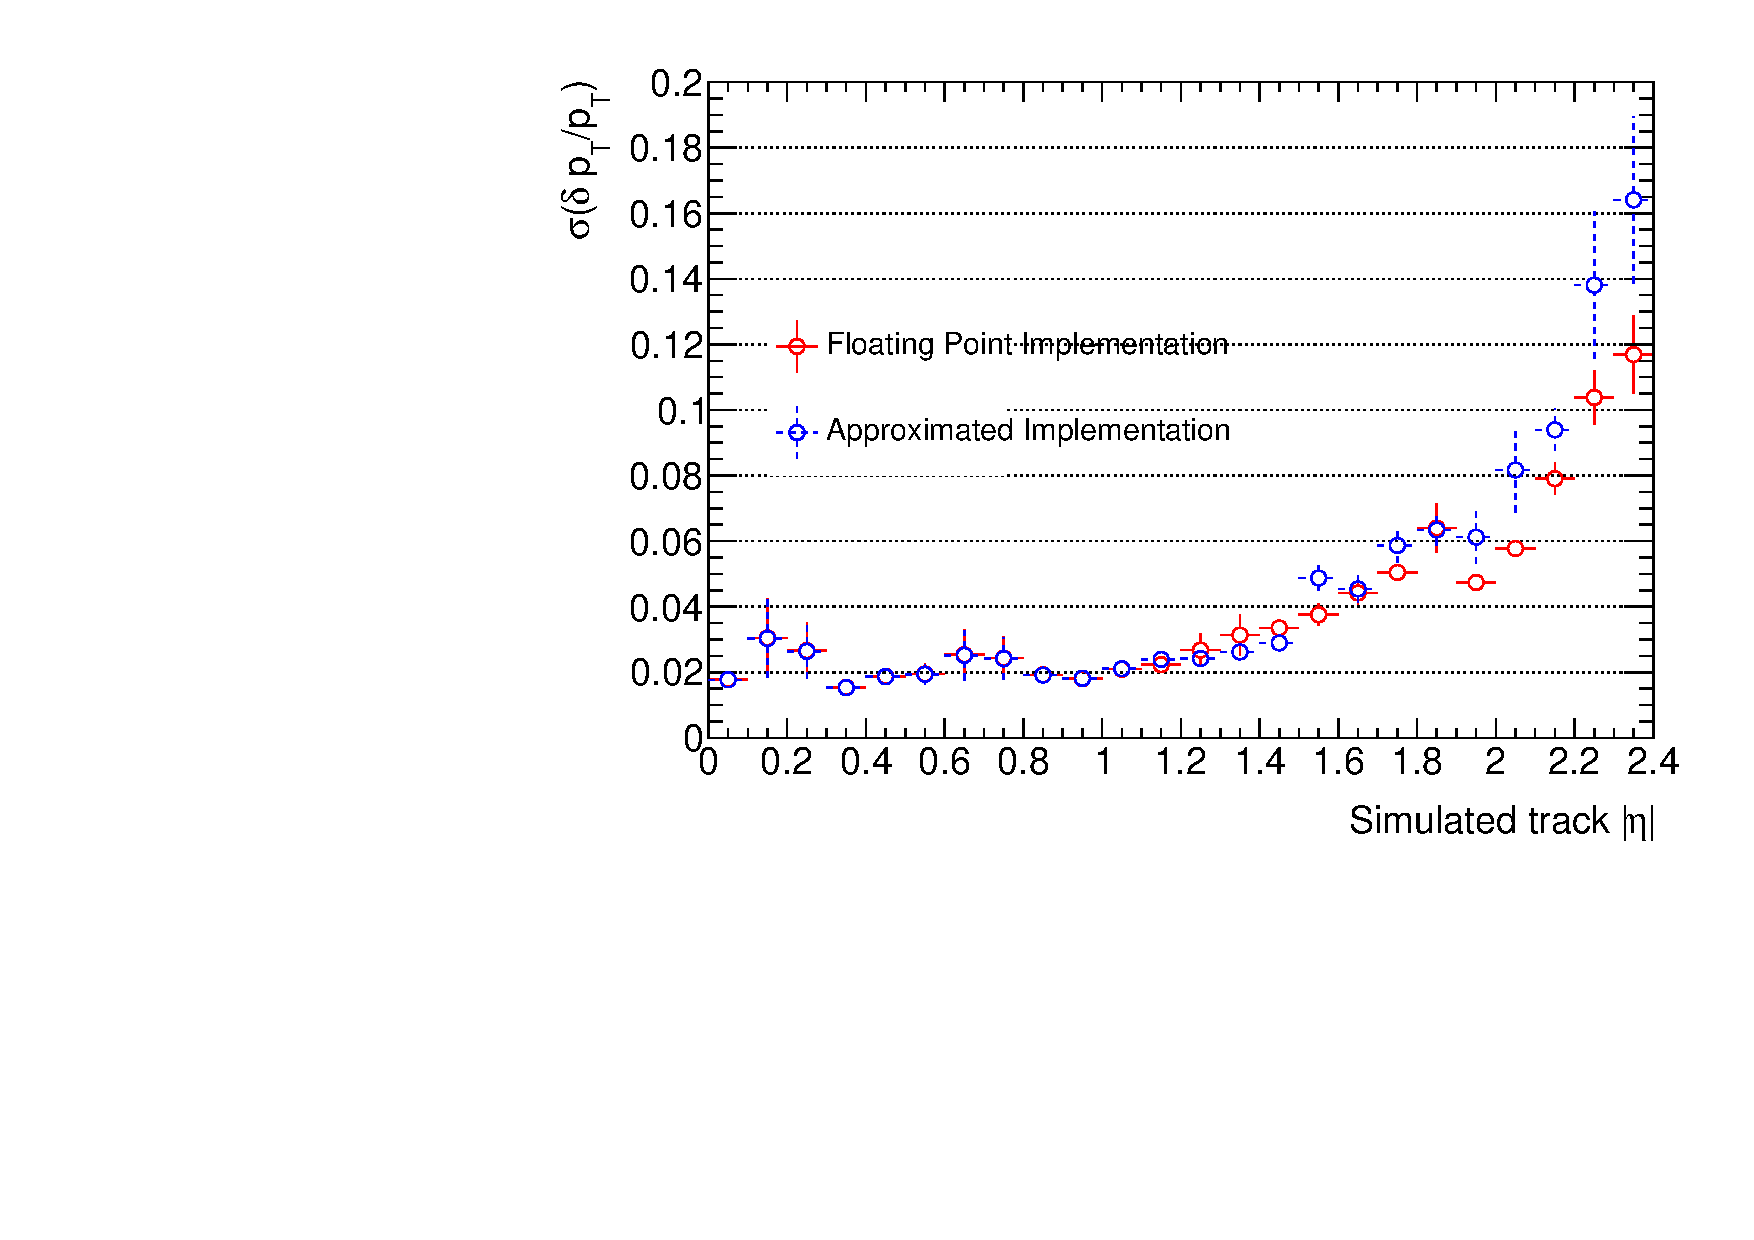
\includegraphics[width=0.49\textwidth]{figs/tk-upgrade/results-chi2fitter/ptRelResVsEta_It_1_ApproxVsExact.pdf}
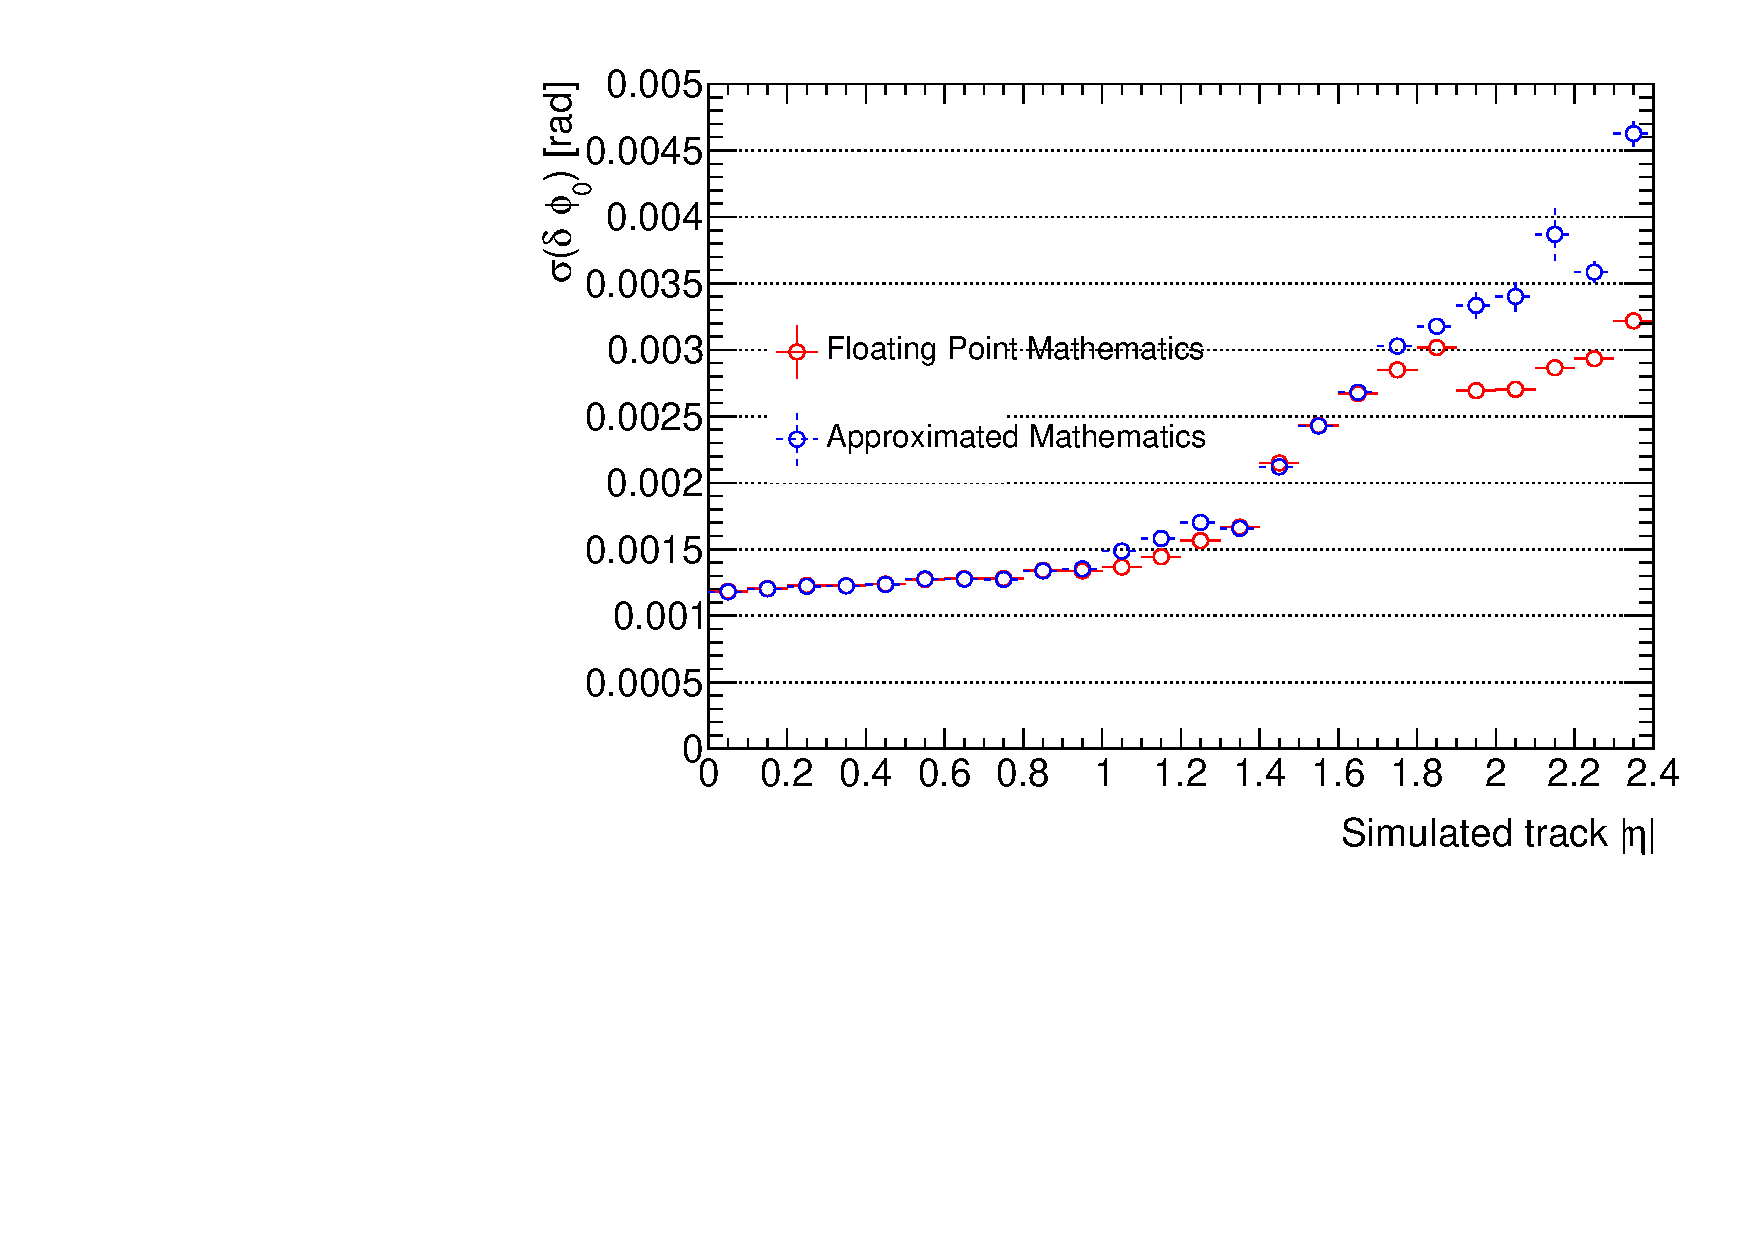
\includegraphics[width=0.49\textwidth]{figs/tk-upgrade/results-chi2fitter/phi0ResVsEta_It_1_ApproxVsExact.pdf}
\\
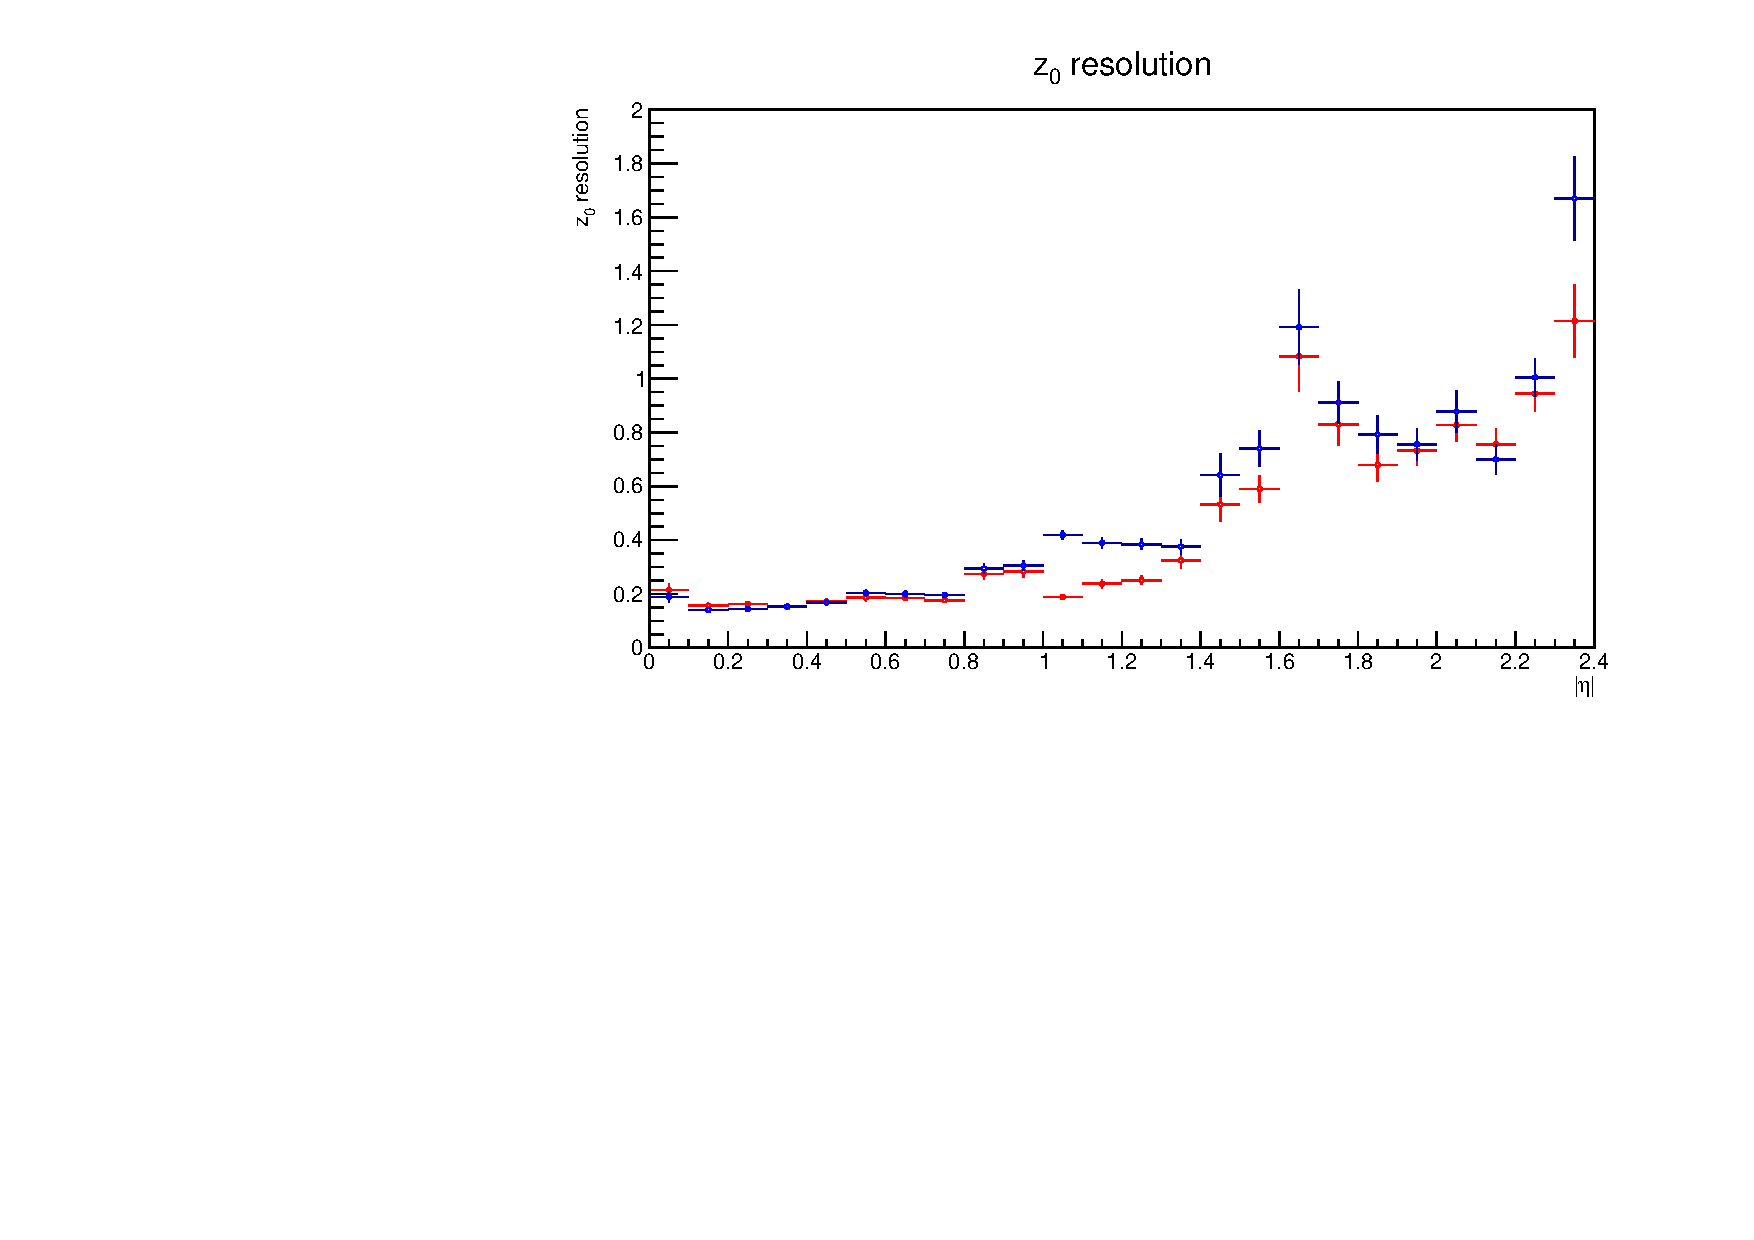
\includegraphics[width=0.49\textwidth]{figs/tk-upgrade/results-chi2fitter/z0ResVsEta_It_1_ApproxVsExact.pdf}
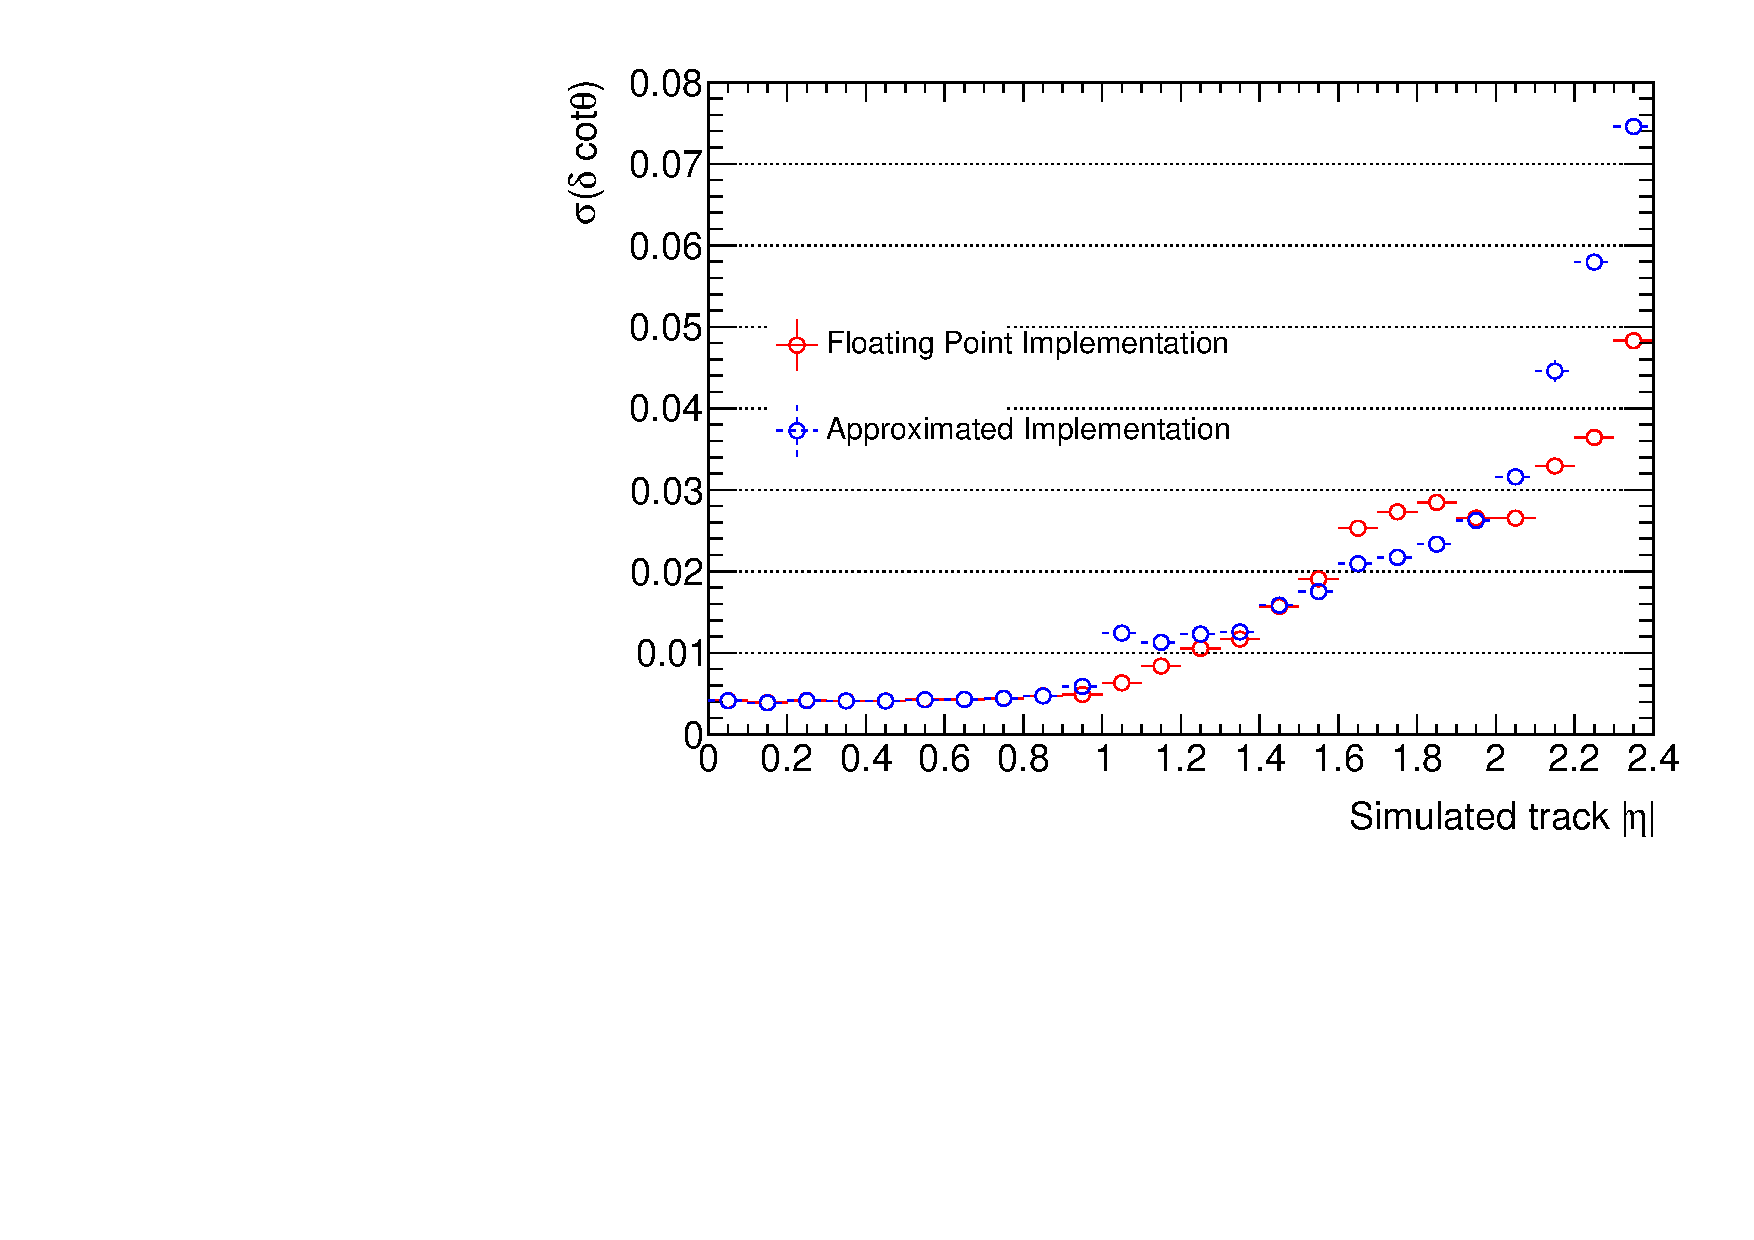
\includegraphics[width=0.49\textwidth]{figs/tk-upgrade/results-chi2fitter/cotThetaResVsEta_It_1_ApproxVsExact.pdf}
\caption{
\pt relative resolution, $\phi$ resolution, $z_{0}$ resolution and $cot(\theta)$ resolution measured for primary reconstructed tracks in simulated \ttbar events at a <PU> of 200 for the floating point (red) and approximated maths (blue) implementations of the linearised $\chi^{2}$ fit algorithm for a single fitting iteration.
\editComment{Make plots bigger!}
}
\label{fig:chi2HelixParametersResVsEtaApproxVsExact}
\end{figure}

%Running multiple iterations of the fitting algorithm had been previously been considered in the context of improving upon the resolution of a fitted track's helix parameters, but had been shown to produce only marginal improvements.

Figure~\ref{fig:chi2HelixParametersResVsEtaApproxVsExact} shows that resolutions of the four track parameters as a function of $\eta$ from primary tracks in \ttbar events at a <PU> of 200 for both mathematical implementations of the algorithm.
The resolutions compare well not just between the two implementations of the algorithm's mathematics, but also with those obtained for the barrel region with the offline track reconstruction which is able to use all information from the detector with more sophisticated reconstruction techniques ~\cite{P2TrackerTDR}.
While this guarantees that the tracks found in the the barrel will be useful to the L-1 trigger, the significant presence of at least one stub being incorrectly associated with a matched track in the forward regions, as shown in Table~\ref{tab:chi2-exactVsApprox}, significantly degrades the resolution obtained.

In order to filter out these incorrectly assigned stubs from matched tracks, and also remove fake tracks, the residuals calculated for each stub following the fit were considered.
These ``fake'' stubs are expected have large residuals compared to stubs correctly associated to genuine tracks or stubs belonging to a fake track.

Therefore, in order to increase the fake rate and matched track purity:
\begin{itemize}
\item the stub with the worst/largest residual is found;
\item this stub is compared against a configurable cut;
\item the stub is removed from the track if its residual exceeds the cut value;
\item the track is refitted using its remaining stubs;
\item and the process is repeated until the latency budget is exceeded/no further stubs are removed, with no further consideration of the remaining stubs' residuals following the final cut.
\end{itemize}

During the optimisation of the cut for this stub quality check it was found that a track could end up having fewer than the minimum of four stubs required to be considered track candidate - thus potentially discarding a matched track by mistake!
To avoid this happening while retaining the improved matched track purity and reduced rate of fake tracks, a looser residual cut was applied for tracks only containing four stubs.

\begin{table}[htbp]
\topcaption {Track finding performance on simulated \ttbar events at a <PU> of 200, for the $\chi^{2}$ track fit using approximated calculations of the track derivatives for when one to four fitting iterations are undertaken. 
The results of further fitting iterations are not shown as they show no further improvement by any metric.
The track finding efficiencies following each stage are given using the efficiency definitions given in Section~\ref{subsec:helixParameter}, along with the mean number of tracks and the fraction of those tracks which are either fake or duplicate tracks.
\editComment{Fix table size}
}
\label{tab:chi2_iterations}
  \centering
% This increases column spacing.
  \resizebox{\textwidth}{!}{
% This right-aligns numbers in column, but centers them under column title.
 \begin{tabular}{ccccccc}
   \hline
   \bf{Track Fitter} & [\#] of iterations & \bf{Efficiency [\%]} & \bf{``Perfect'' Efficiency [\%]} & \bf{Mean [\#] of tracks} & \bf{Fakes [\%]} & \bf{Duplicates [\%]}  \\
   \hline
   $\chi^{2}$+DR & 1 & 94.9 & 85.6 & 87.4 & 15.5 & 10.9 \\  
   & 2 & 93.8 & 91.0 & 73.8 & 6.6 & 7.7 \\
   & 3 & 93.1 & 91.0 & 71.4 & 5.3 & 6.9 \\
   & 4 & 93.0 & 91.0 & 71.1 & 5.2 & 6.8 \\
   \hline
   KF+DR & - & 94.1 & 94.1 & 82.1 & 21.1 & 4.5 \\
   \hline
   
 \end{tabular}}
\end{table}

Table~\ref{tab:chi2-exactVsApprox} illustrates how the tracking performance of the linearised $\chi^{2}$ fitter improves with just one additional fitting iteration (removal of a stub), with the fake rate halving and matched track purity noticeably improving, albeit at the expense of the looser definition of the track finding efficiency.
Further successive fitting iterations yield diminishing returns, with no further improvements seen following four fitting iterations.
Given that the mean number of hits associated to a track is seven, the majority of tracks can only have up to three stubs removed.
By contrast, while a greater number of fake tracks survive the \KF's filtering, the \KF achieves a similar tracking efficiency as two iterations of the $\chi^{2}$ fitter whilst none of the matched tracks found contain any incorrect stubs. 
This suggests that if a more sophisticated method of removing bad quality stubs were used in the linearised $\chi^{2}$ fitter, then  not many matched tracks would be discarded while their purity would be increased.
Although such an improvement may come at the expense of a low fake rate, such tracks can be potentially cleaned further downstream but tracks which aren't reconstructed are lost forever.

Figure~\ref{fig:chi2HelixParametersResIterationsComparison} shows helix parameter resolution differences between one and four fitting iterations of the $\chi^{2}$ fitter, allowing for the removal of zero and up to three stubs respectively, and how this compares against the \KF's performance.
The additional fitting iterations allow for noticeable improvements for the track parameter resolutions obtained in the forward regions.
While the \qpt and $\phi_{0}$ resolutions achieved after four fitting iterations is comparable to those achieved by the \KF, the $\chi^{2}$ fitter's resolution is considerably worse for both the $z_{0}$ and $cot(\theta)$ resolutions in the endcaps.

\begin{figure}[htb]
\centering
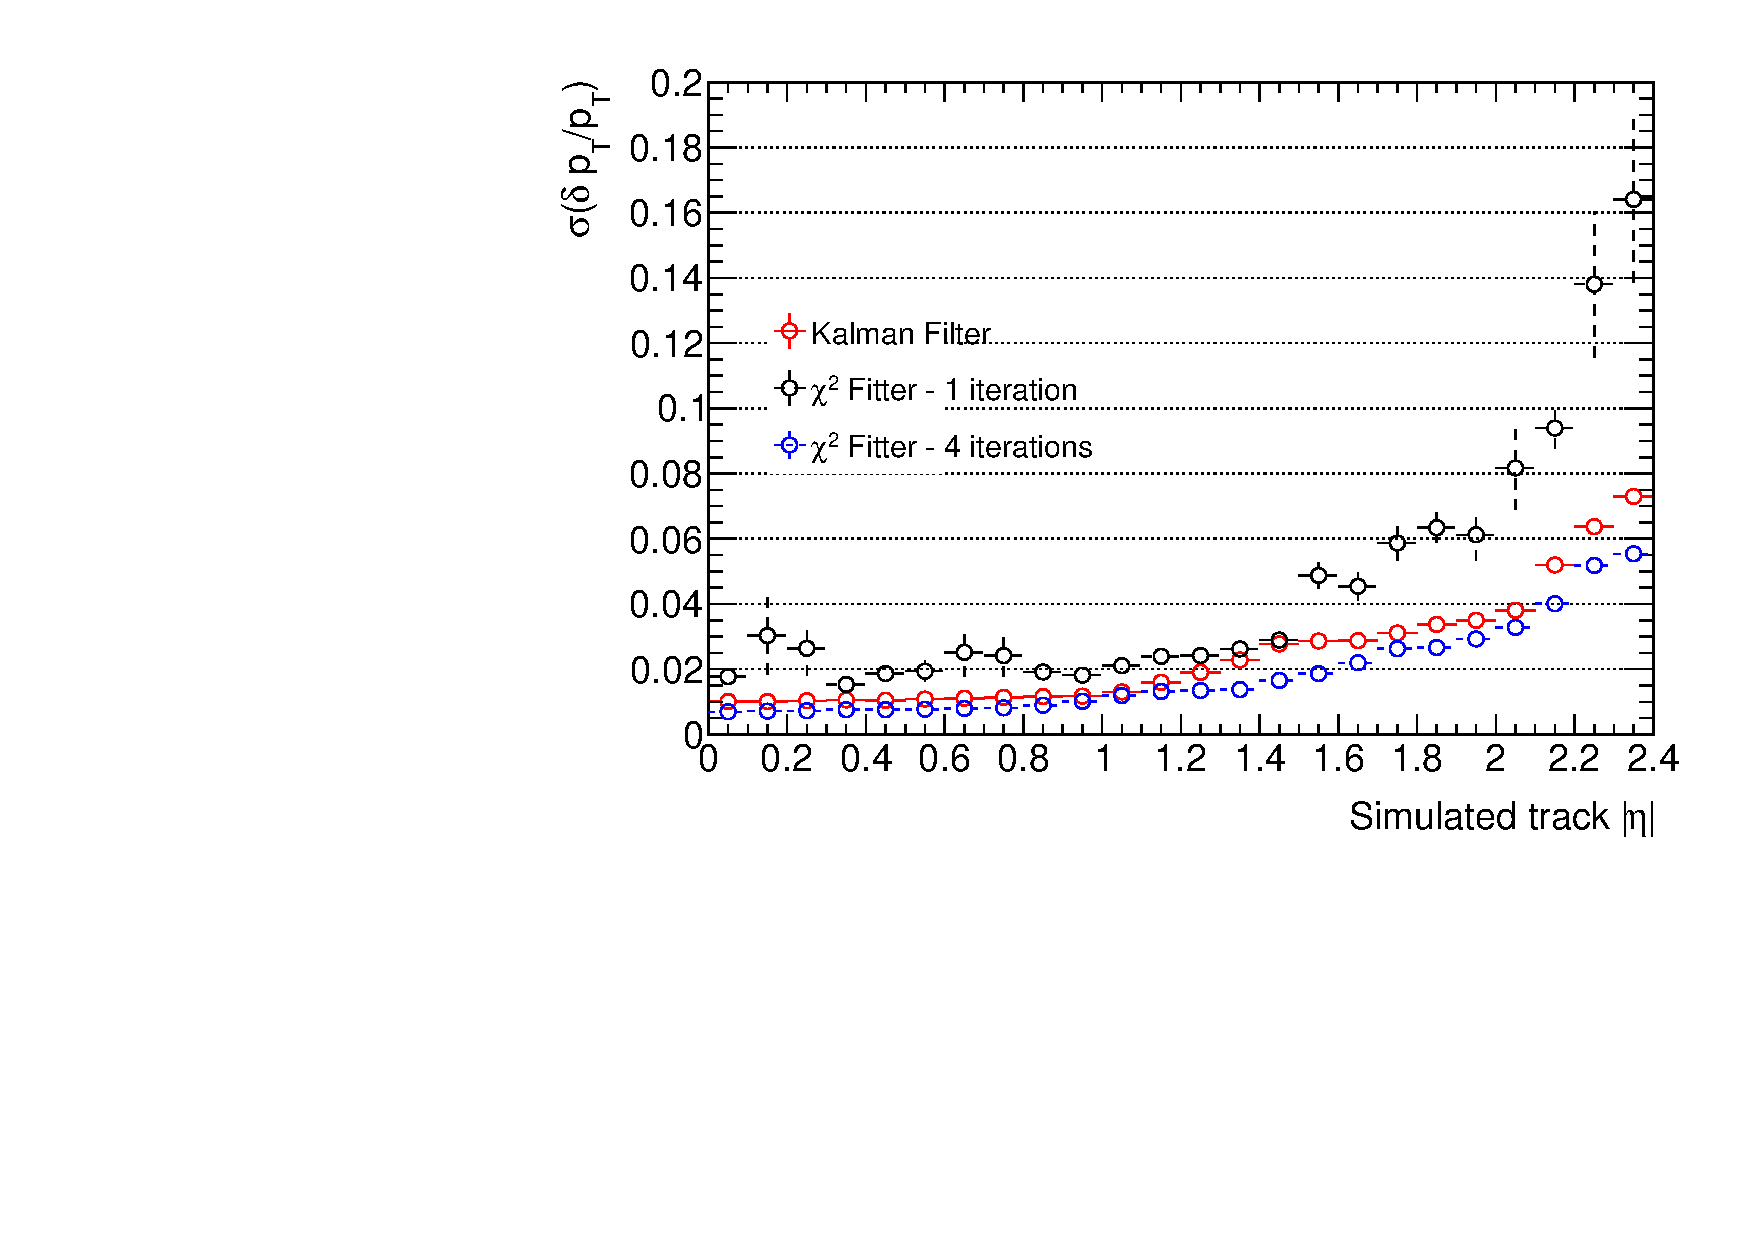
\includegraphics[width=0.49\textwidth]{figs/tk-upgrade/results-chi2fitter/ptRelResVsEta_IterationComparison.pdf}
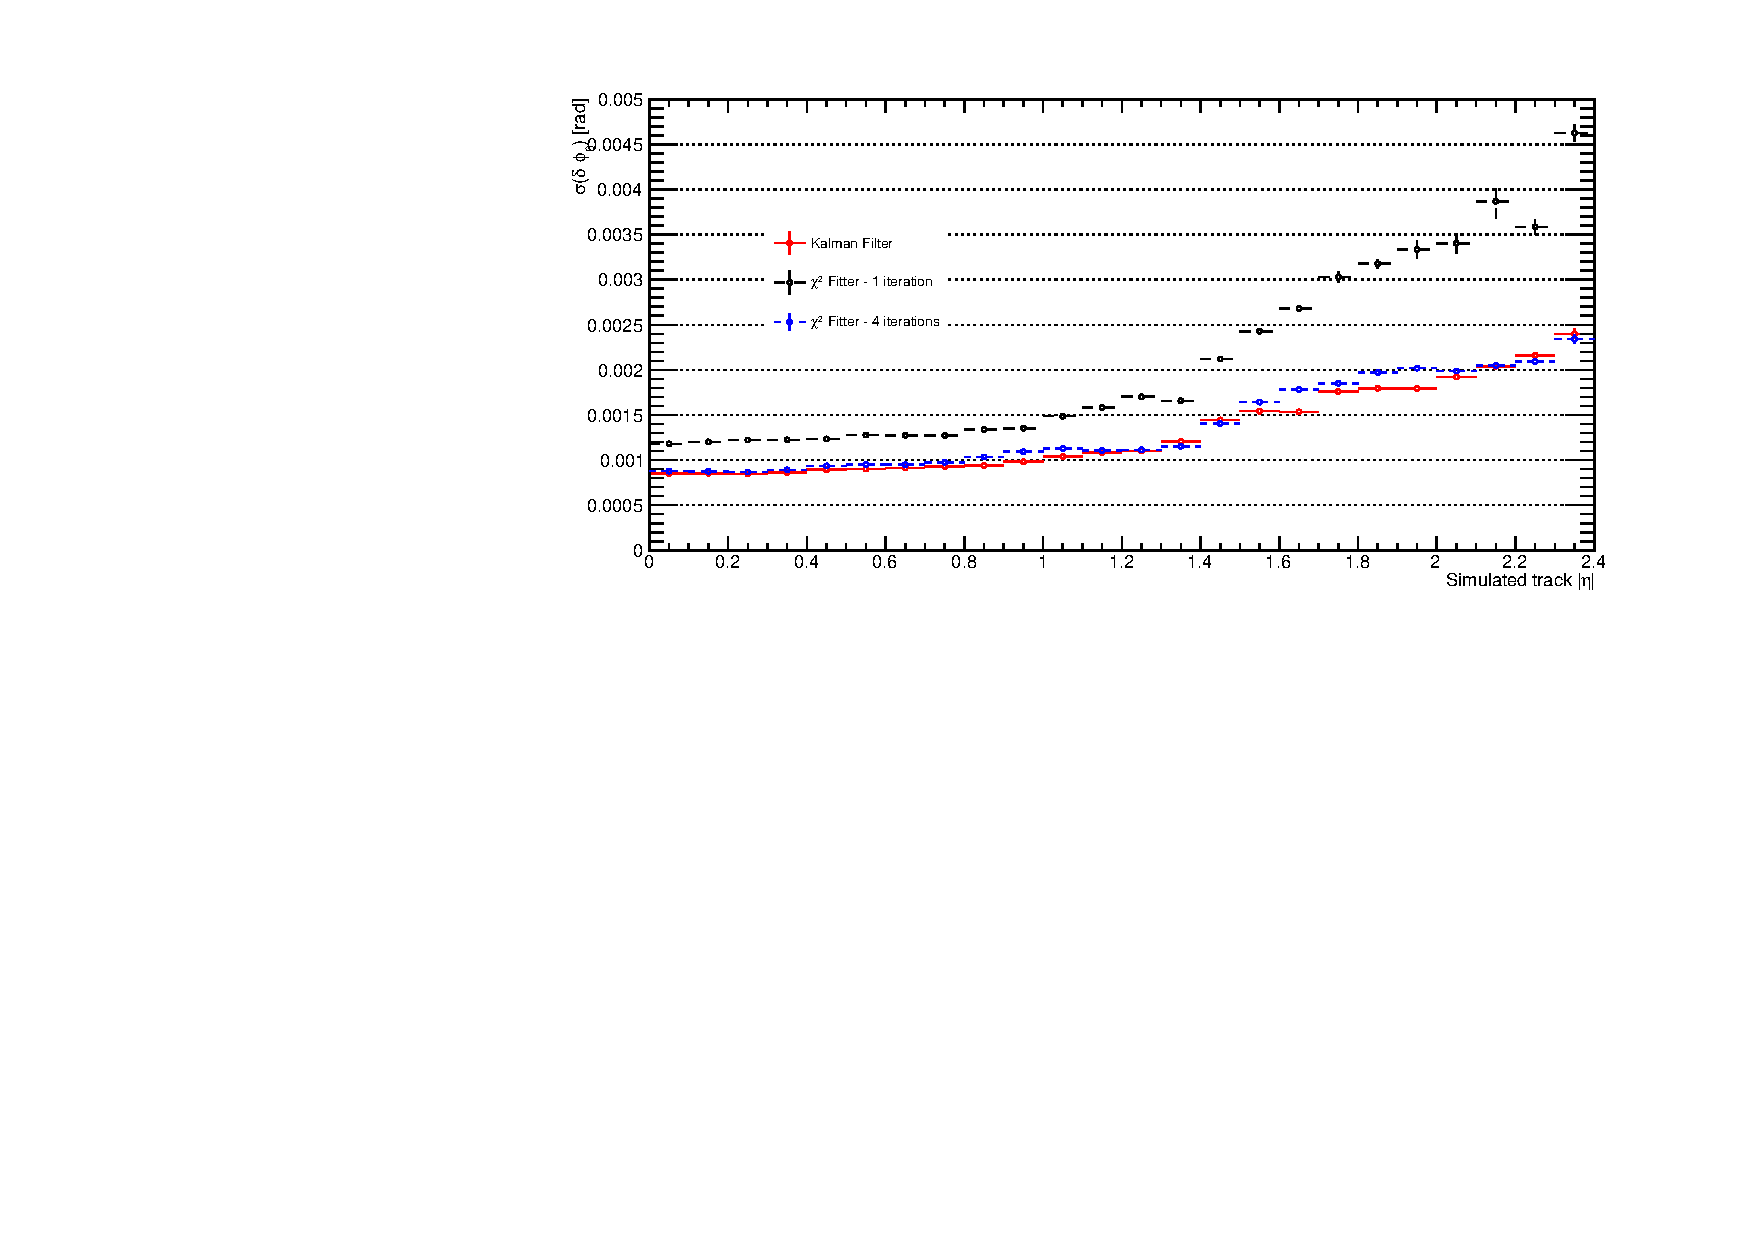
\includegraphics[width=0.49\textwidth]{figs/tk-upgrade/results-chi2fitter/phi0ResVsEta_IterationComparison.pdf}
\\
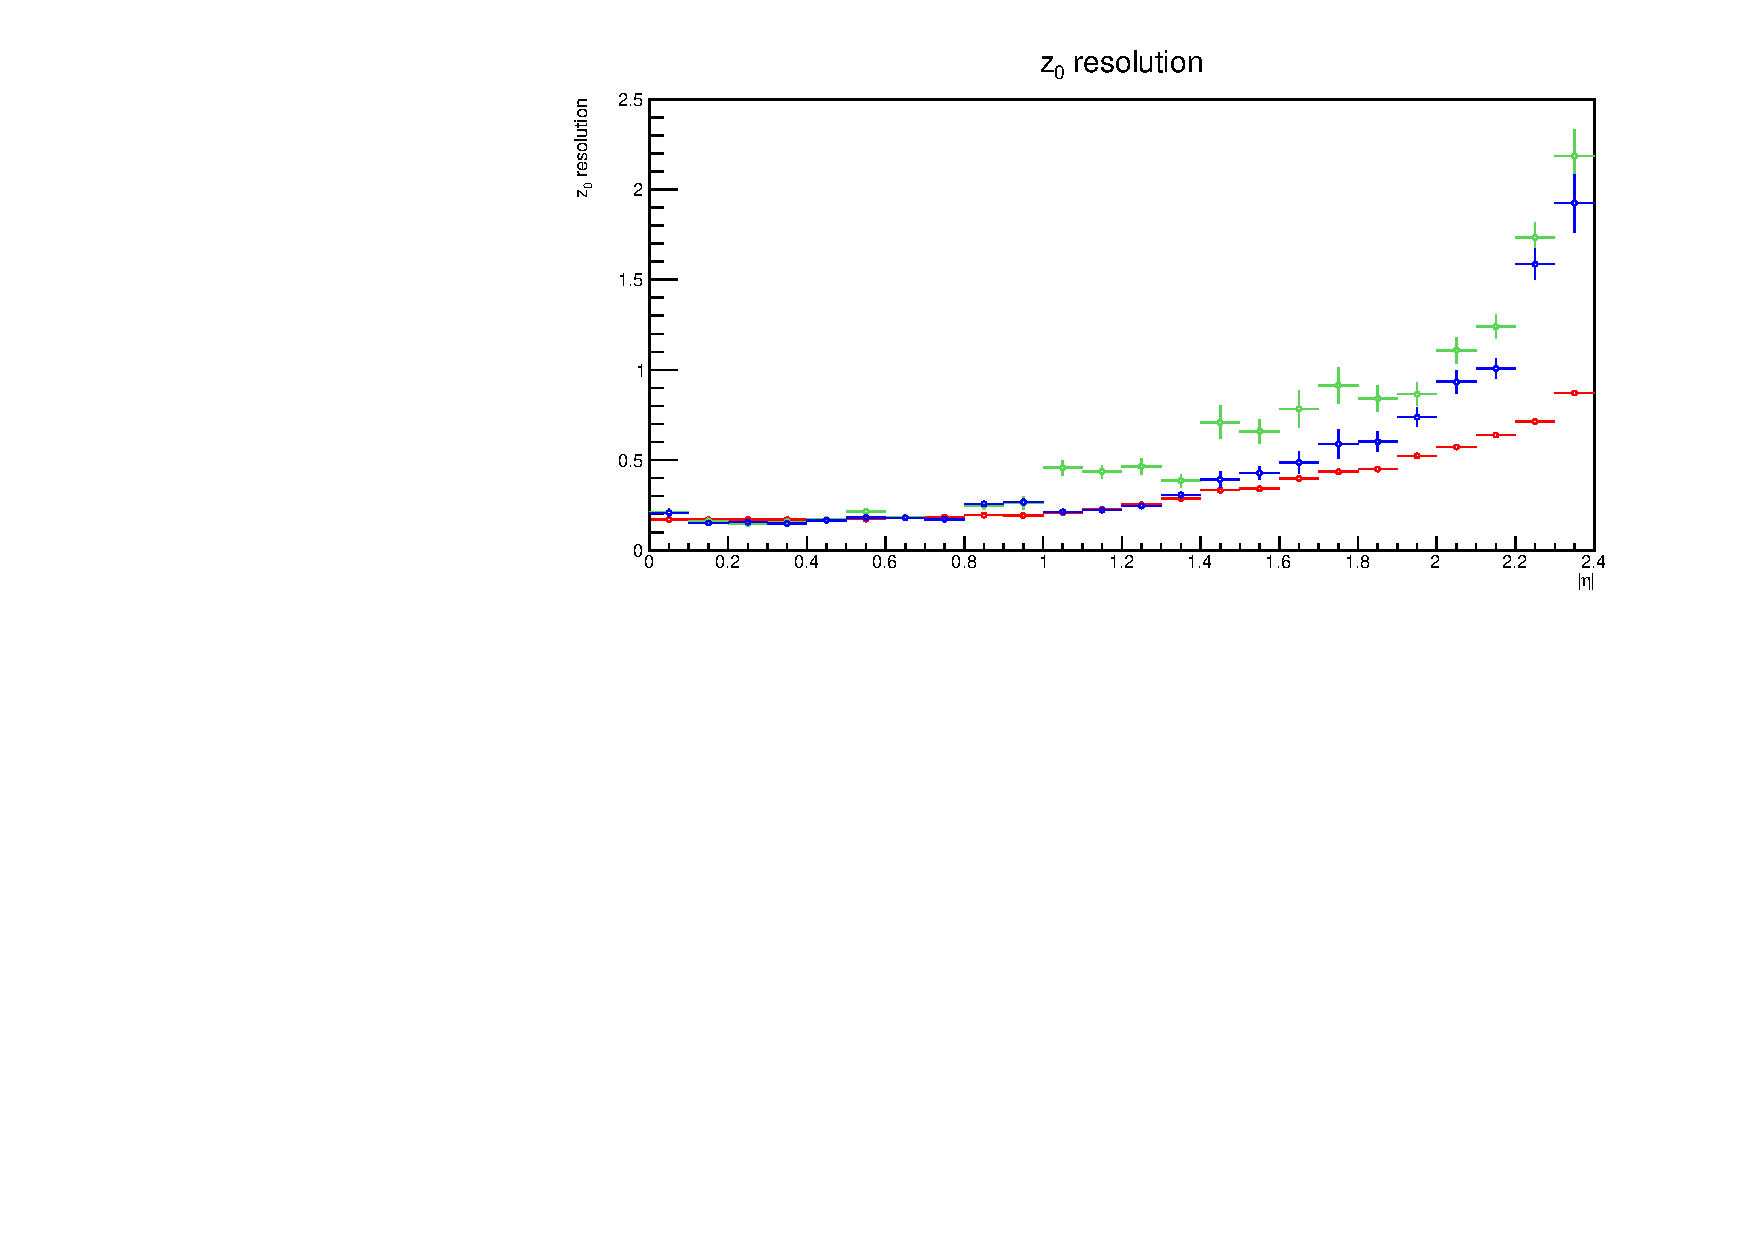
\includegraphics[width=0.49\textwidth]{figs/tk-upgrade/results-chi2fitter/z0ResVsEta_IterationComparison.pdf}
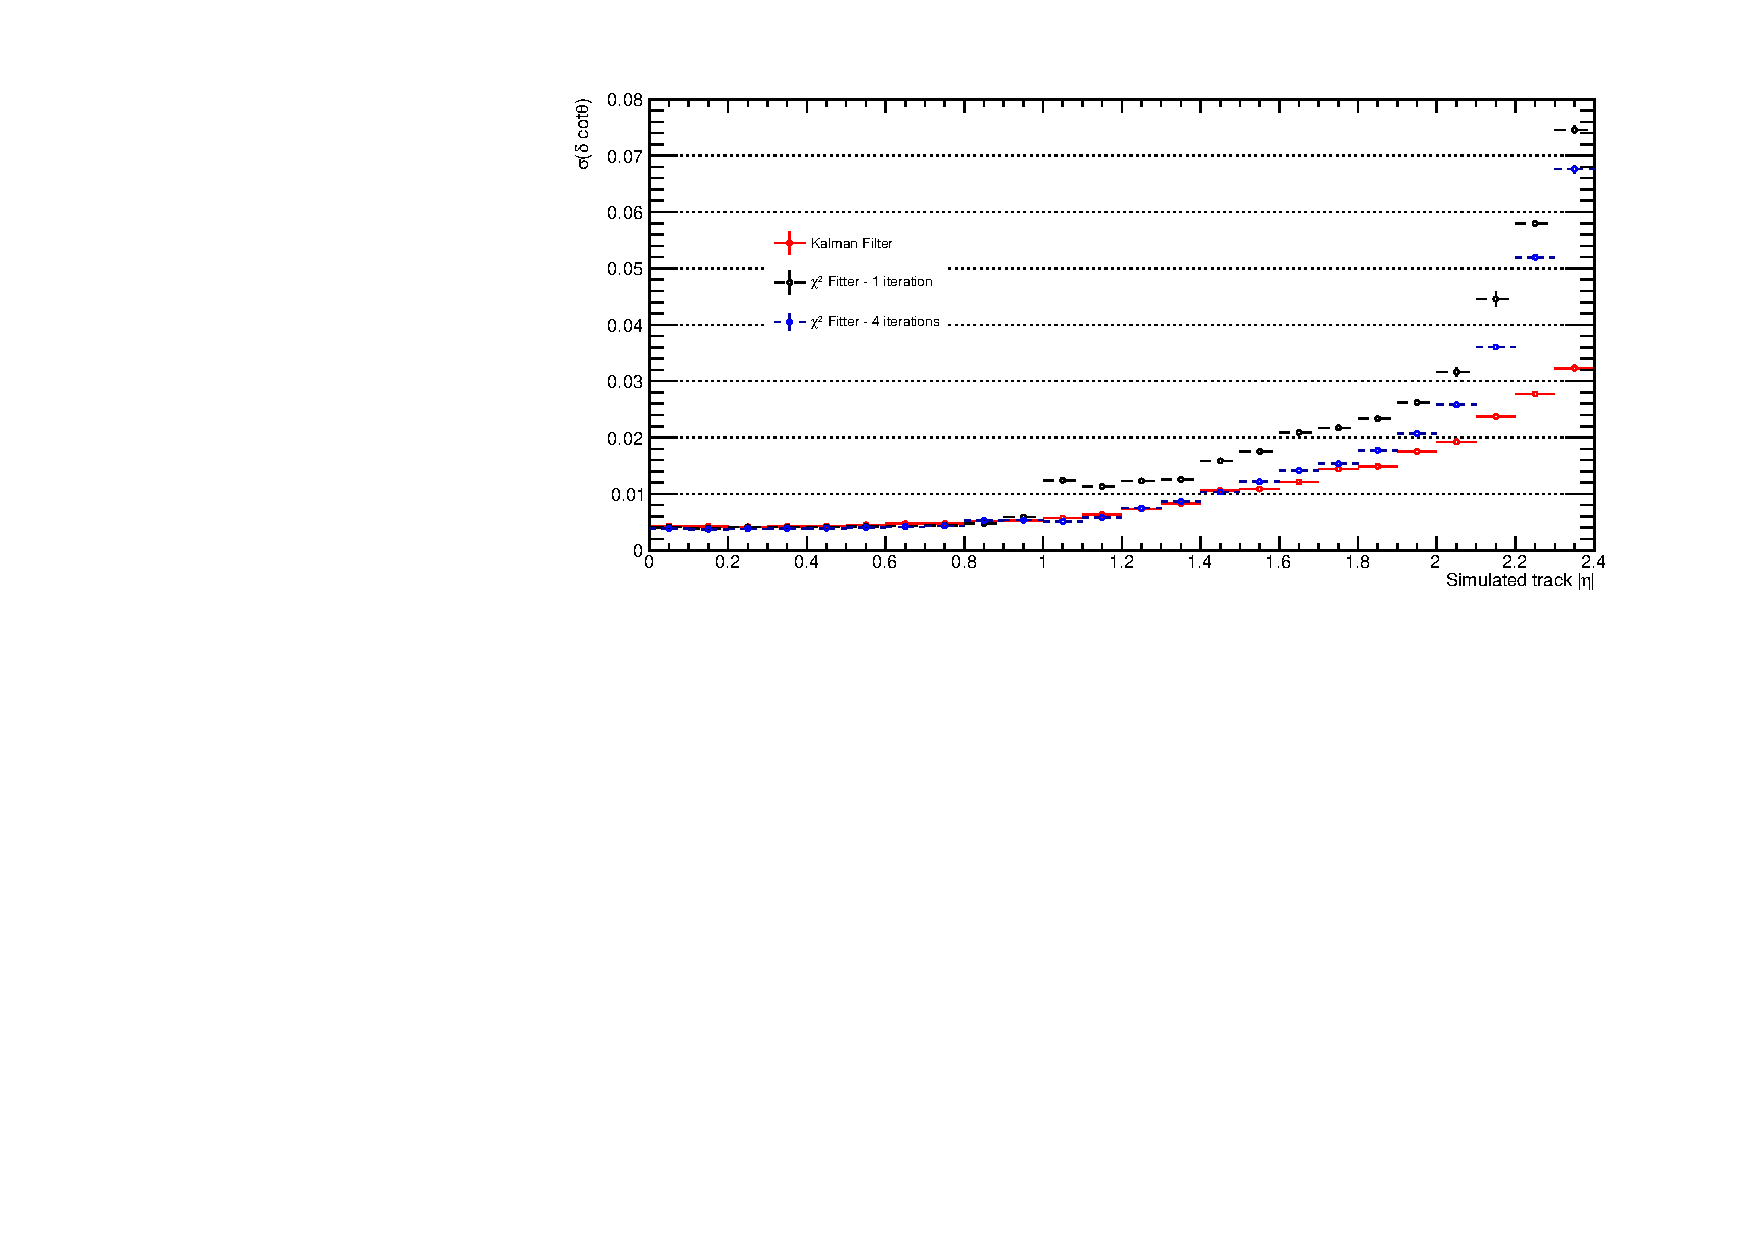
\includegraphics[width=0.49\textwidth]{figs/tk-upgrade/results-chi2fitter/cotThetaResVsEta_IterationComparison.pdf}
\caption{
\pt relative resolution, $\phi$ resolution, $z_{0}$ resolution and $cot(\theta)$ resolution measured for primary reconstructed tracks in simulated \ttbar events at a <PU> of 200 for the approximated maths implementation of the linearised $\chi^{2}$ fit algorithm for one (black) and four (blue) fitting iterations. The \KF (red) is also included for comparison.
\editComment{Make plots bigger!}
}
\label{fig:chi2HelixParametersResIterationsComparison}
\end{figure}

\subsubsection{Conclusions and Outlook}\label{subsubsec:chi2outlook}
\editComment{Polish more}
A linearised $\chi^{2}$ track fit has been implemented in software in an form using approximated mathematics to simplify any potential tabulation of its derivatives and a set of internal cuts which are iteratively applied to remove fake stubs from matched tracks and reject fake tracks.
Following the parallel development of both the linearised $\chi^{2}$ track fit and the \KF however, it was decided that development on the former would be discontinued in favour of focussing resources on the latter.
The motivations behind this decision were that the \KF was capable of achieving a higher track finding efficiency with 100.0\% purity for matched tracks, superior $z_{0}$ and $cot(\theta)$ resolutions in the endcaps which were comparable to the offline resolution and that considerable progress had been made with an implementation in firmware.
In contrast, the linearised $\chi^{2}$ track was not competitive in terms of track resolution and reconstruction ability, especially with respect to the stricter tracking efficiency definition, and there were also concerns over the potential feasibility of tabulating all (or the most frequently used) track derivatives in the endcap disks for FPGAs which were commercially available at the time.

\subsection{Tracking at low transverse momentum}\label{subsec:Tmtt2GeV}
The flexibility to reconstruct tracks down to a lower \pT threshold of 2\GeV may be desirable if the trigger requirements demand it, so the impact of this potential requirement on the proposed proposed track-finder system was studied.
These studies were initially undertaken as part of the the robustness studies required for the 2016 demonstrator review, focussing on recovering tracking efficiency below 3\GeV with the \HT, and were subsequently built upon with modifications to the \KF algorithm after 2016.
The results relating to \HT modifications were produced prior to the conclusion of the demonstrator review and were produced using the flat barrel geometry, and the results for the \KF improvements produced with the tilted barrel geometry.
As the number and width of the \qpt \HT columns used varies from the standard fixed number and size of columns typically used, thus varying the \pT resolution available, the track parameters are expressed as a function of 1/\pT instead of \pT.

\subsubsection{Hough Transform Optimisation}\label{subsubsec:lowPtOptHT}
Lowering the \HT \pT threshold from 3\GeVc to 2\GeVc required modifying the GP and HT configuration parameters to ensure adequate duplication in $\phi$ and increasing the number of the \qpt columns by 50\% to take into account the increased \pt range whilst maintaining the same precision.
The increased number of \qpt columns has the impact of increasing the required FPGA resources by 50\% and the output data rate from the \HT by a factor of 2.2.

Without any further modifications, there is a considerable degradation in the track reconstruction efficiency by the \HT in the range $2\GeVc < \pt < 2.7\GeVc$, due to these low momenta tracks being dominated by multiple scattering.
This results in stubs not always intersecting within a single \HT cell and thus failing to exceed the threshold criteria and generate track candidates.
To mitigate against such track reconstruction efficiency losses, using a preexisting feature which had been separately implemented in firmware, the precision of the \HT cells along \qpt and $\phi_{T}$ for the range $2\GeVc < \pt < 2.7\GeVc$ was reduced by a factor of two (\ie $2 \times 2$ cells were merged).
Additionally, the \KF state $\chi^2$ cuts for this low \pT range were optimised to reflect the increased hit position uncertainty resulting from the decreased precision of the hits in these \HT cells and thus reduce the number of duplicate and fake tracks as far as possible without impacting on the \HT track reconstruction efficiency.
Figure~\ref{fig:2GeVFlatEff} shows how the tracking efficiency improves following the use of the variable precision \HT with and without optimised \KF state cuts after both the \HT and the full demonstrator chain. 

\begin{figure}[tbp]
\centering
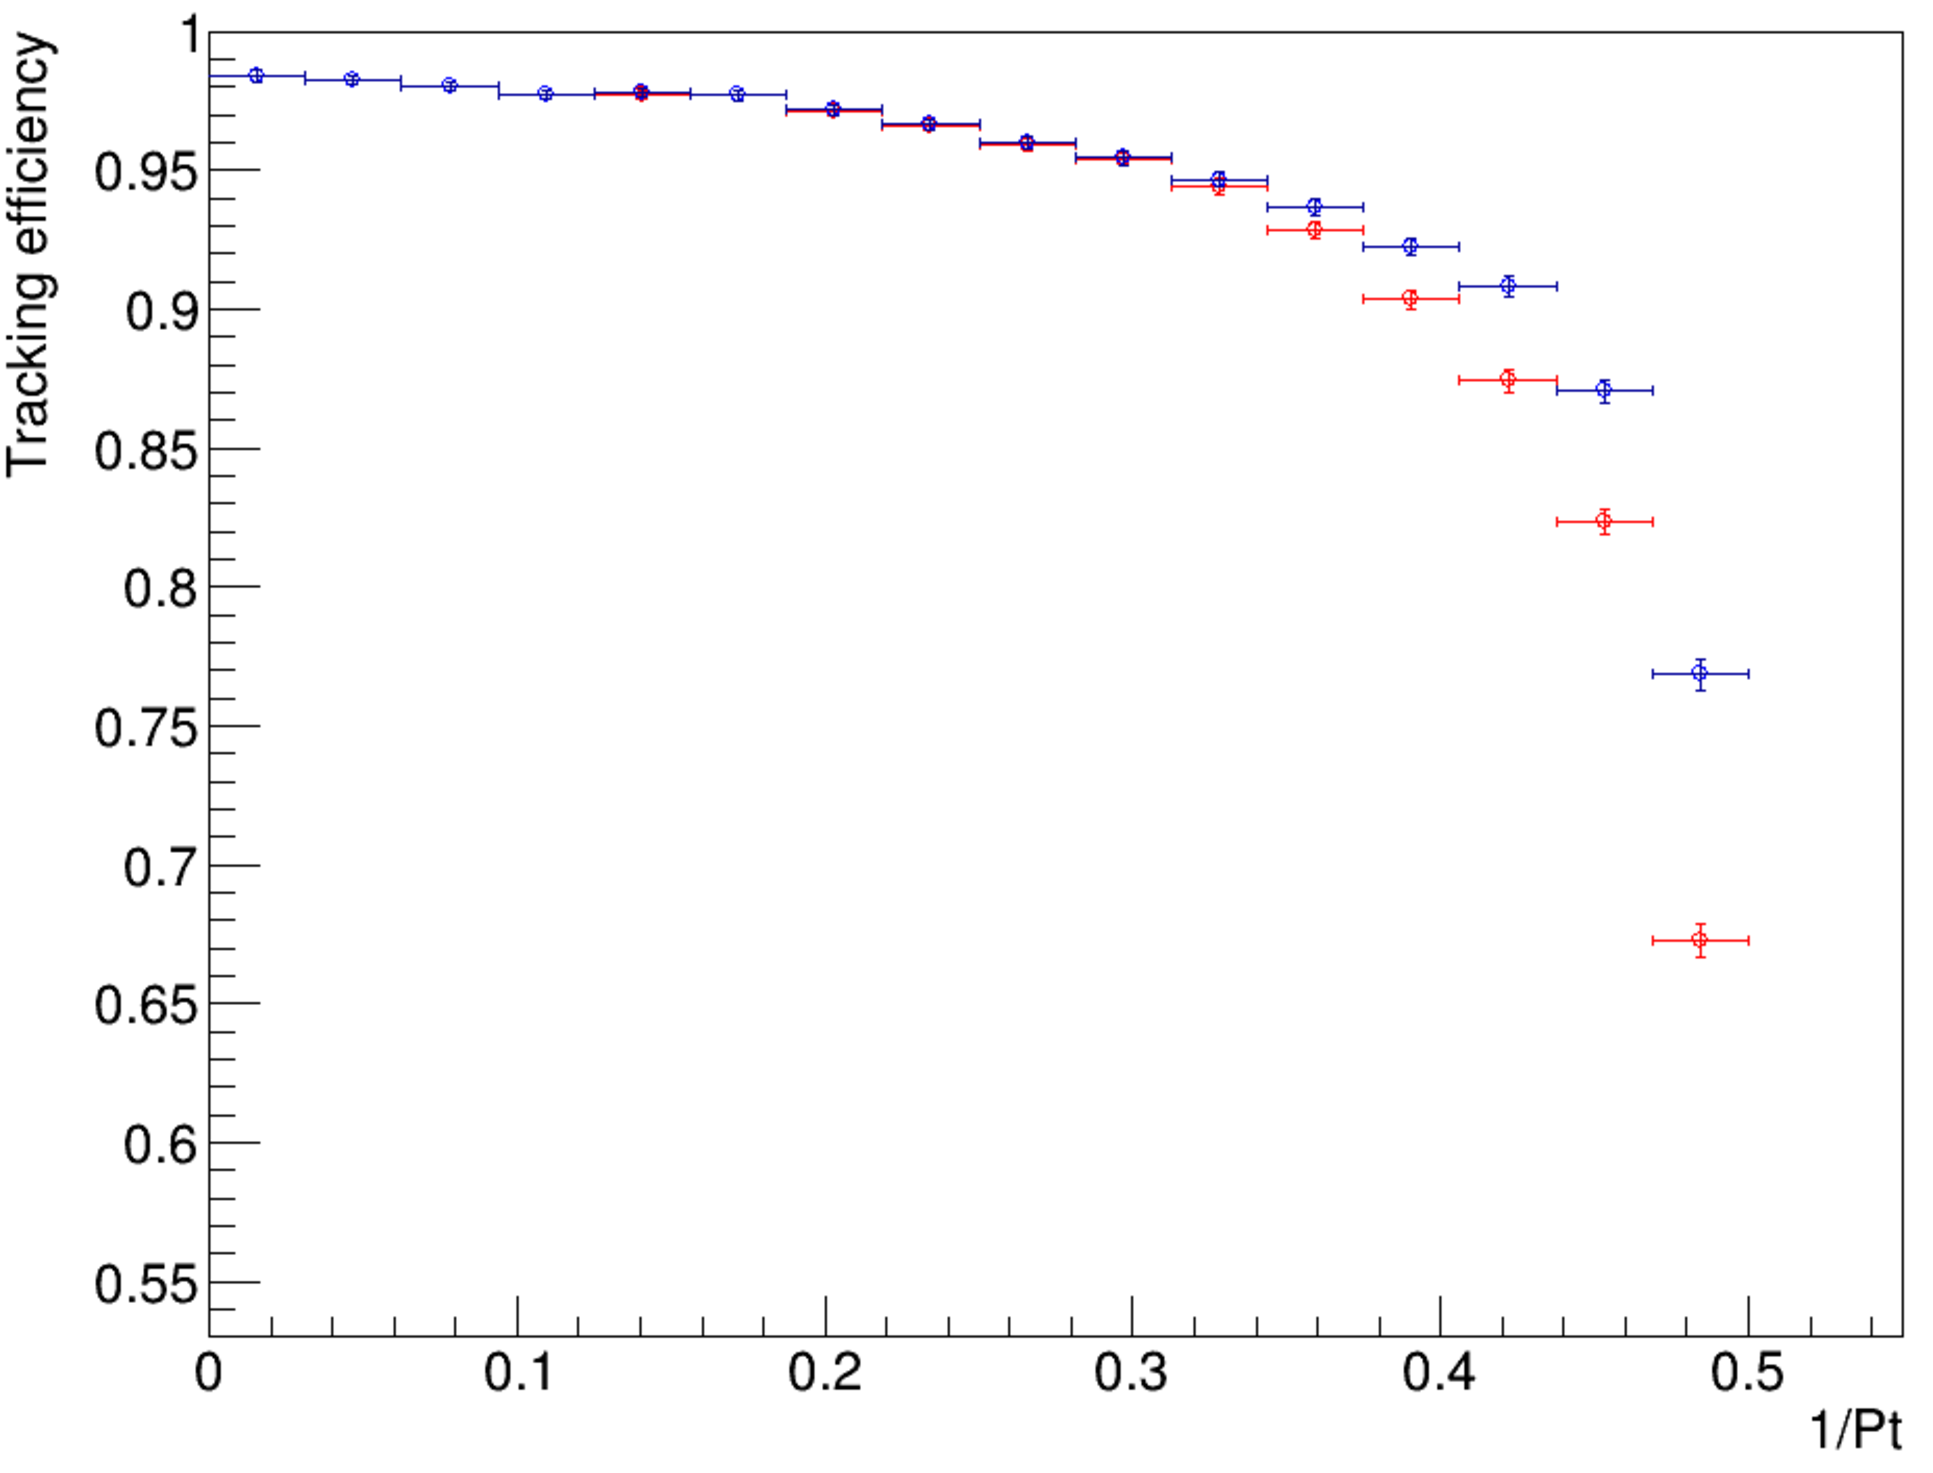
\includegraphics[width=0.49\textwidth]{figs/tk-upgrade/results-lowPtTracking/htTrackingEffVsInvPtFlatGeometry_5000.pdf}
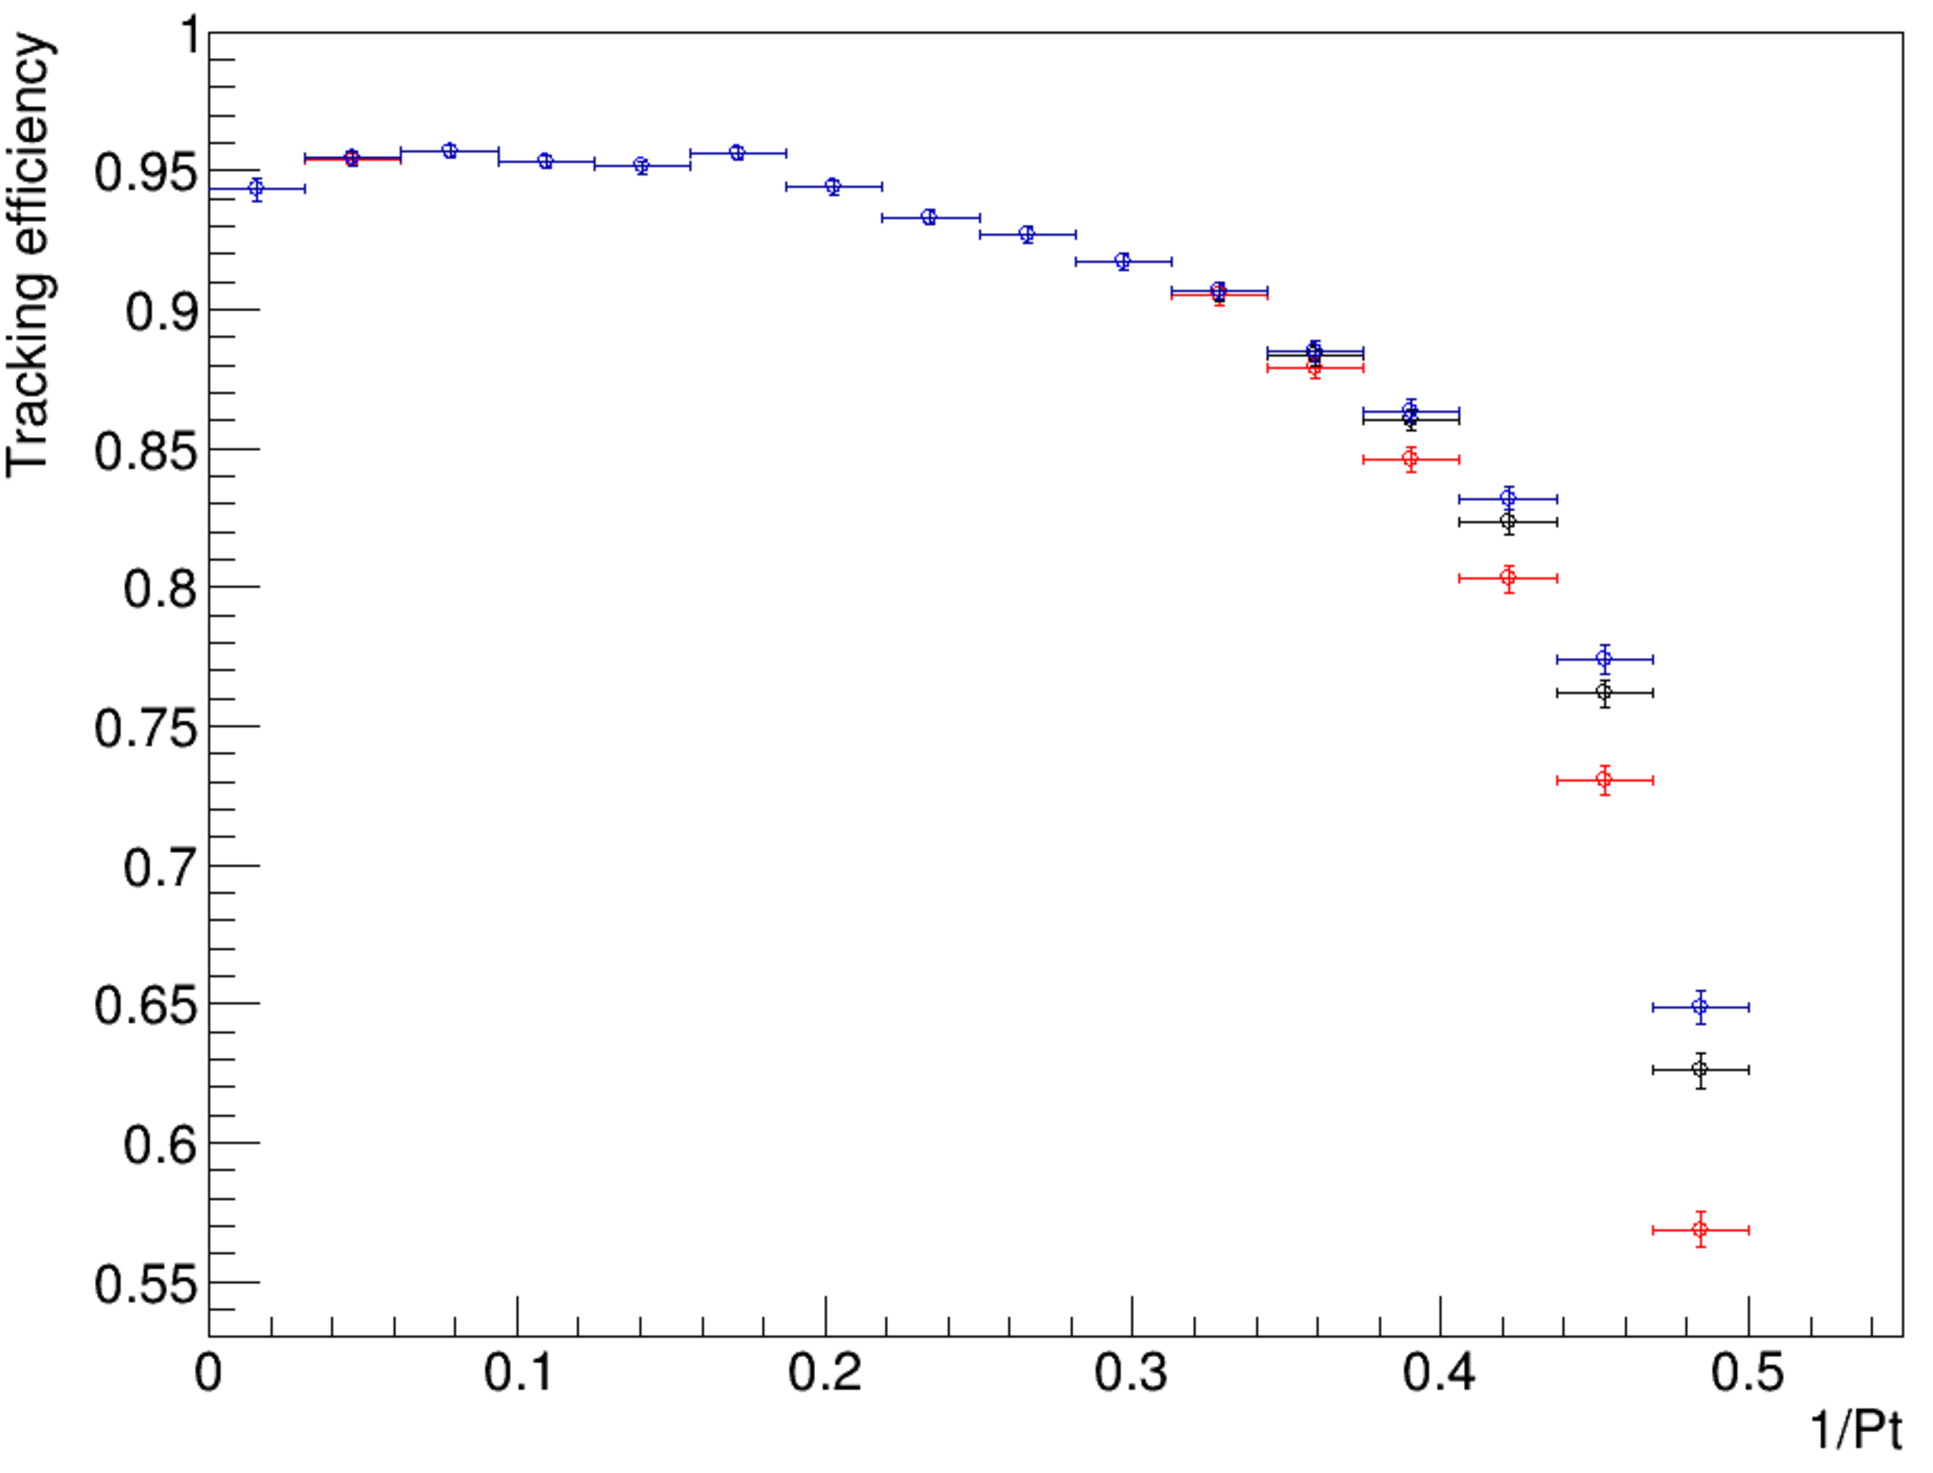
\includegraphics[width=0.49\textwidth]{figs/tk-upgrade/results-lowPtTracking/kfTrackingEffVsInvPtFlatGeometry_5000.pdf}
\caption{The post-\HT (left) and post-\KF (right) tracking efficiency for $\pt > 2\GeVc$ for \ttbar events at a <PU> of 200, with the default configuration where only the number of \qpt columns are increased (red) and with the increased number of columns, HT cell merging and \KF state cuts optimisation(blue).
}
\label{fig:2GeVFlatEff}	
\end{figure}

%%% Disucss table here
Table~\ref{tab:trackFindingPerformance2GeVHT} shows the impact that the decreased precision \HT cells and optimised \KF state cuts have on tracking performance both following the \HT and the full chain.
It is clear that whilst the merging of adjacent \HT cells recovers  tracks which did not previously intersect within a single \HT cell, the tracking efficiency following the full chain is significantly less than that post-\HT.
As shown in figure~\ref{fig:2GeVFlatEff}, these losses occur for tracks where the particle's transverse momentum is less than 3\GeV, as the \KF does not take the effects of \MS into account.
This shortcoming of the \KF also accounts for it not being as efficient at removing fake tracks, with an observed increase of 5\% in the fraction of fakes reconstructed.
The duplicate removal algorithm however, remains effective at removing almost all the duplicates.

\begin{table}[htbp]
\topcaption {Track finding performance on simulated \ttbar events at a <PU> of 200, after the \HT and the full chain  for the configurations of only increasing the number of \qpt columns (\emph{Default}), additionally using \HT cell merging and the optimised \KF state cuts (\emph{Optimised}).
The track finding efficiencies following each stage are given using the efficiency definitions given in Section~\ref{subsec:helixParameter}, along with the mean number of tracks and the fraction of those tracks which are either fake or duplicate tracks.
\editComment{Fix table size}
}
\label{tab:trackFindingPerformance2GeVHT}
  \centering
% This increases column spacing.
  \resizebox{\textwidth}{!}{
% This right-aligns numbers in column, but centers them under column title.
\begin{tabular}{cccccc}
   \hline
   \bf{Configuration} & \bf{Stage} & \bf{Efficiency [\%]} & \bf{Mean \# of tracks} & \bf{Fakes [\%]} & \bf{Duplicates [\%]}  \\
        \hline
    Default & \bf{HT}     & 93.6 & 713.2 & 34.0 & 44.5 \\  
    & \bf{Full chain}     & 89.2 & 193.9 & 21.1 & 5.1 \\      
%   \hline
%    Merge & \bf{HT}     & 94.6 & 799.2 & 40.5 & 39.7 \\  
%    & \bf{Full chain}     & 89.8 & 206.5 & 25.4 & 3.9 \\      
    \hline
    Optimised & \bf{HT}     & 94.6 & 799.2 & 40.5 & 39.7 \\  
    & \bf{Full chain}     & 90.0 & 210.4 & 26.3 & 3.8 \\      
   \hline
   
 \end{tabular}}
\end{table}

The point made about \MS not being properly accounted for in the \KF is illustrated by figure~\ref{fig:2GeVFlatChi2Ndf} which shows the distributions of $\chi^{2}$ per number of degree of freedom ($\frac{\chi^{2}}{ndf}$) as a function of $\frac{1}{\pT}$ for genuine tracks produced by the \KF.
If all uncertainties were accounted for, the ideal distribution of $\frac{\chi^{2}}{ndf}$ would be unity for all \pT, in contrast to the dramatic increase above approximately 3\GeV from the approximately flat distribution at order unity.

\begin{figure}[tbp]
\centering
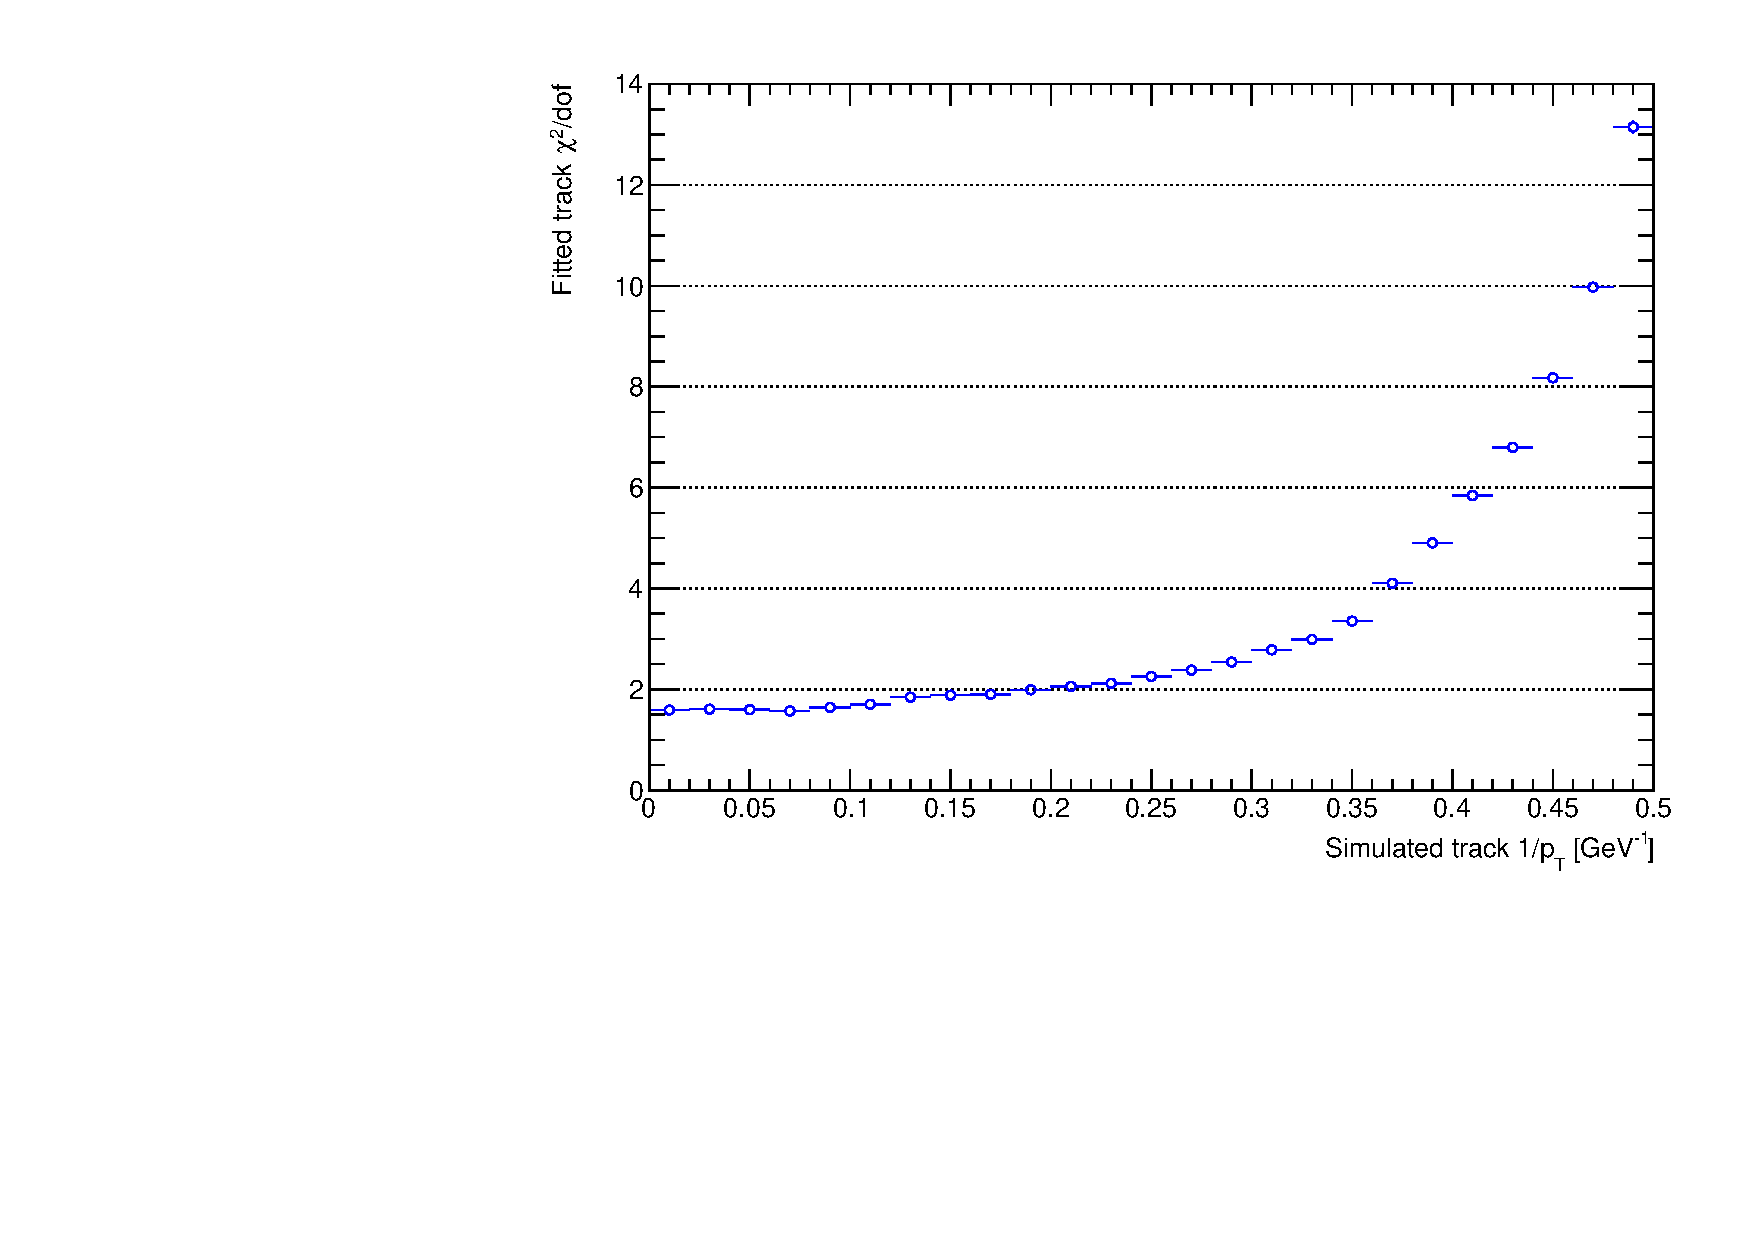
\includegraphics[width=\textwidth]{figs/tk-upgrade/results-lowPtTracking/kfChi2NdfVsInvPtFlatGeometry_5000.pdf}
\caption{Plot of $\frac{\chi^{2}}{ndf}$ as a function of $\frac{1}{\pT}$ for genuine tracks produced by the \KF.}
\label{fig:2GeVFlatChi2Ndf}
\end{figure}

%% Discuss the resolution plots here
Figure~\ref{fig:htHelixParametersResVsInvPt} shows that the resolutions of the track parameters fitted by the \KF are comparable for $\pT < 3\GeV$ for both the default configuration of the \HT where only the number of \qpt columns has been increased and after the \HT and associated \KF optimisations for tracks originating from the primary interaction in \ttbar events at a <PU> of 200.
The slight degradation in the $\phi_{0}$ resolution is a result of the decreased precision coordinates from the \HT and the small improvement observed in the $z_{0}$ resolution is due to the \KF being able to consider genuine stubs which were not previously found by the \HT.

\begin{figure}[htb]
\centering
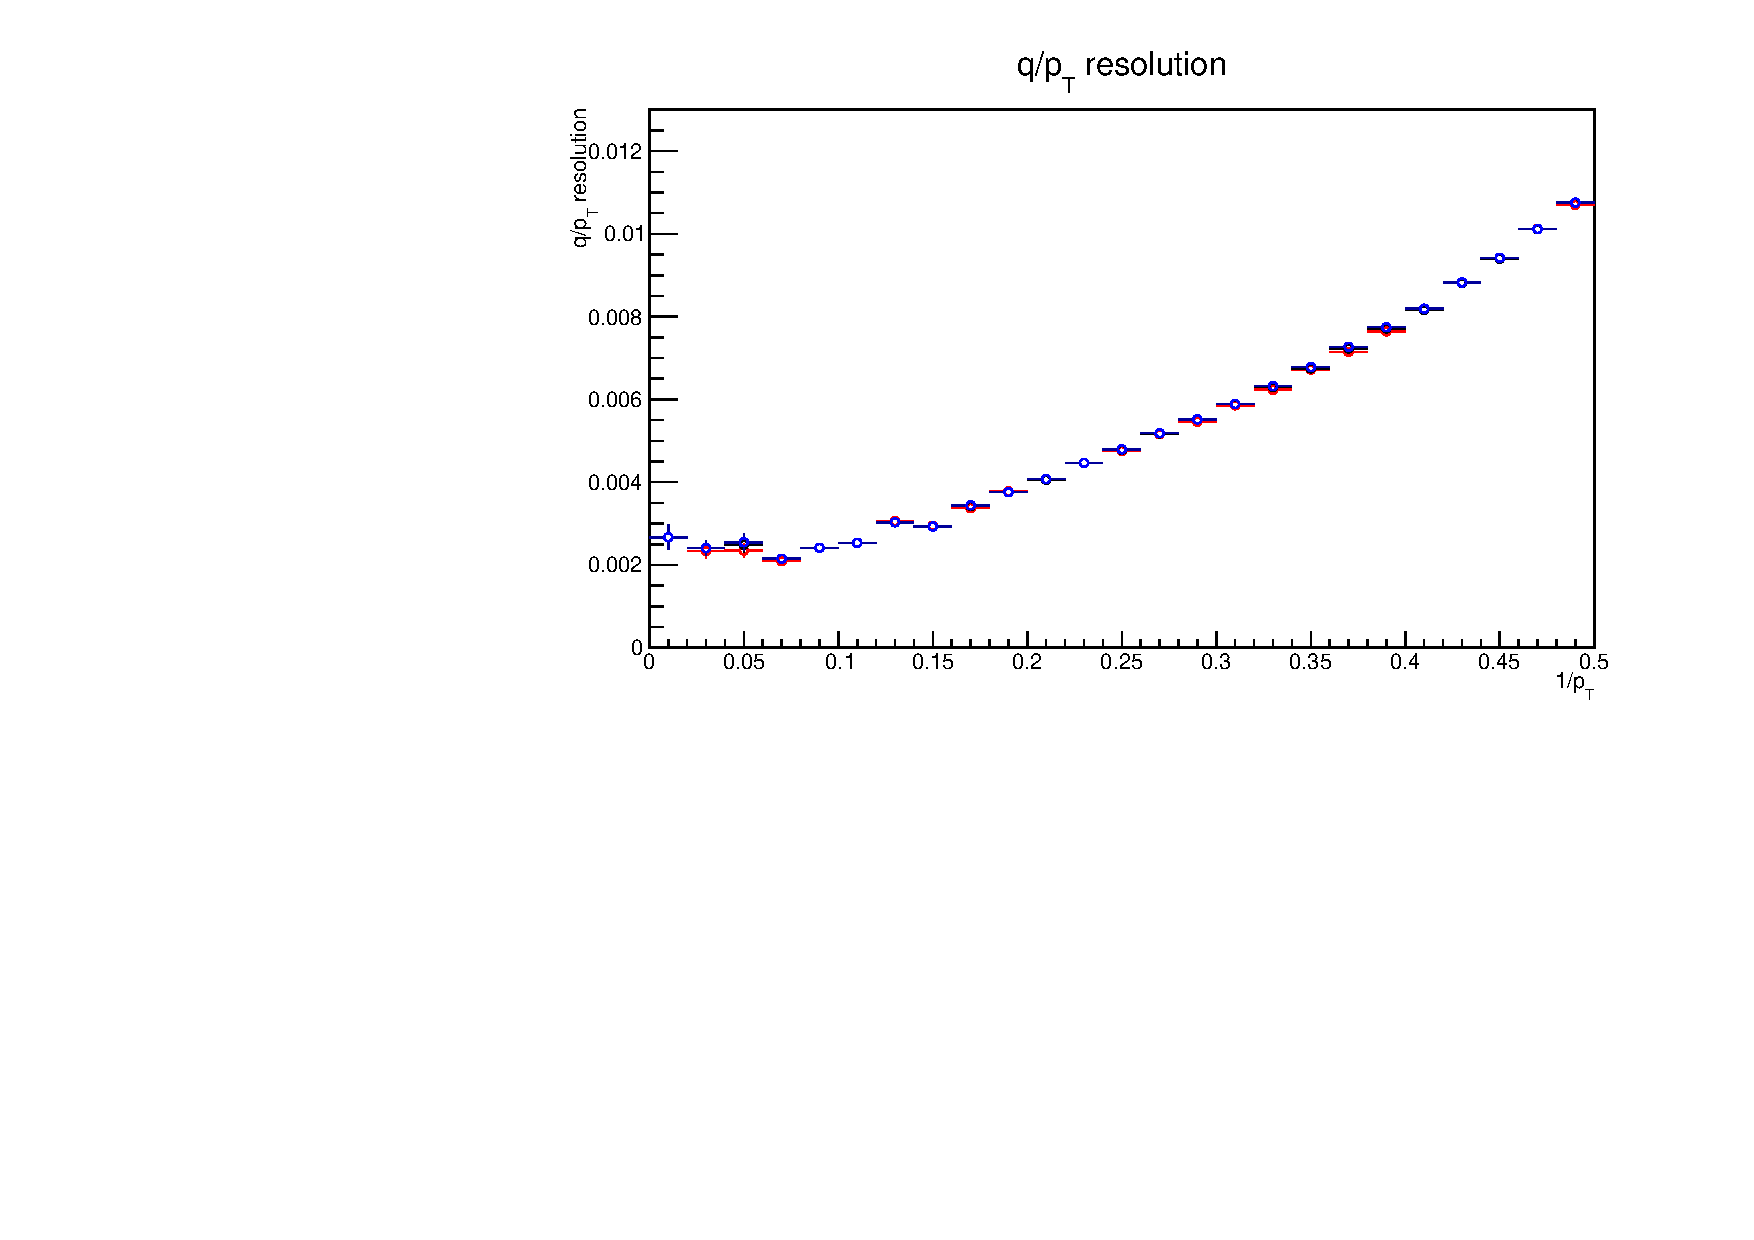
\includegraphics[width=0.49\textwidth]{figs/tk-upgrade/results-lowPtTracking/qOverPtResVsInvPtFlatGeometry_5000.pdf}
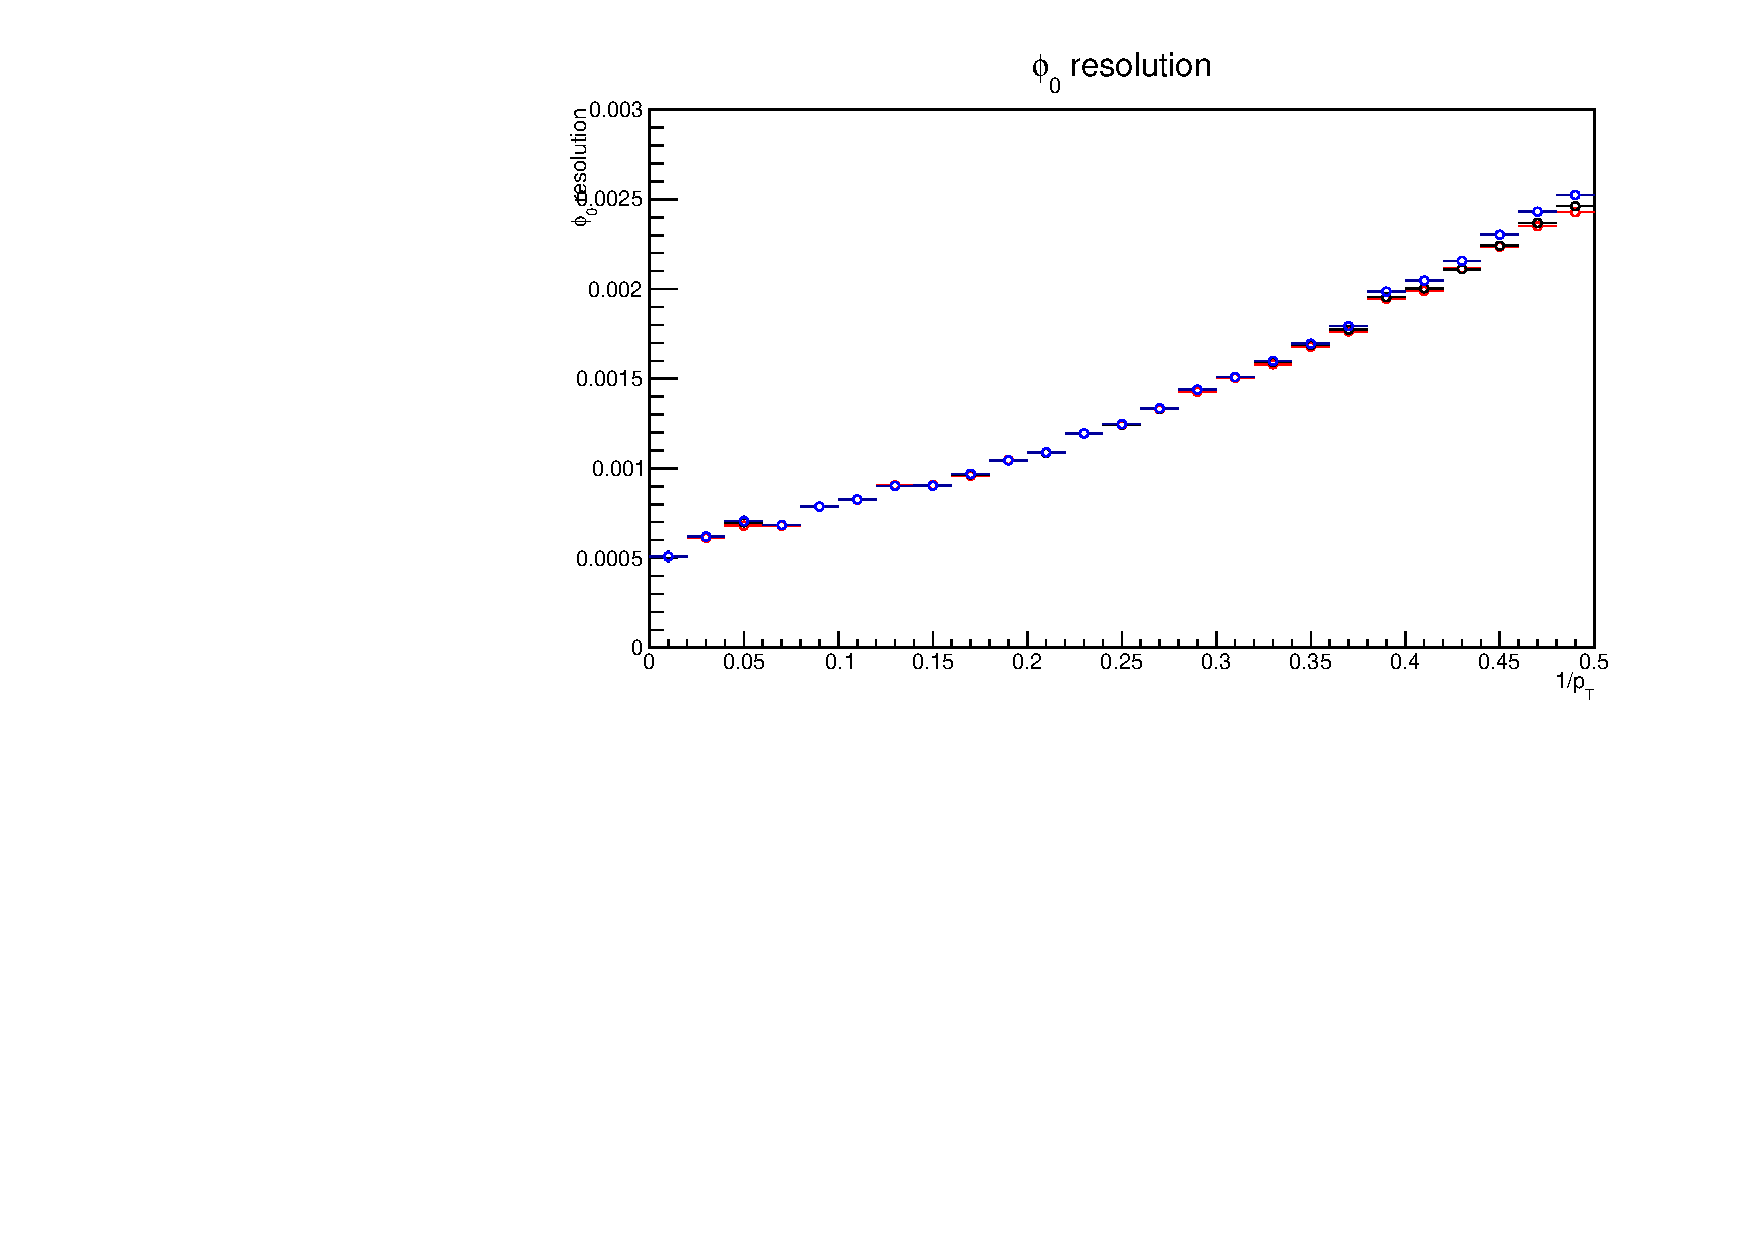
\includegraphics[width=0.49\textwidth]{figs/tk-upgrade/results-lowPtTracking/phi0ResVsInvPtFlatGeometry_5000.pdf}
\\
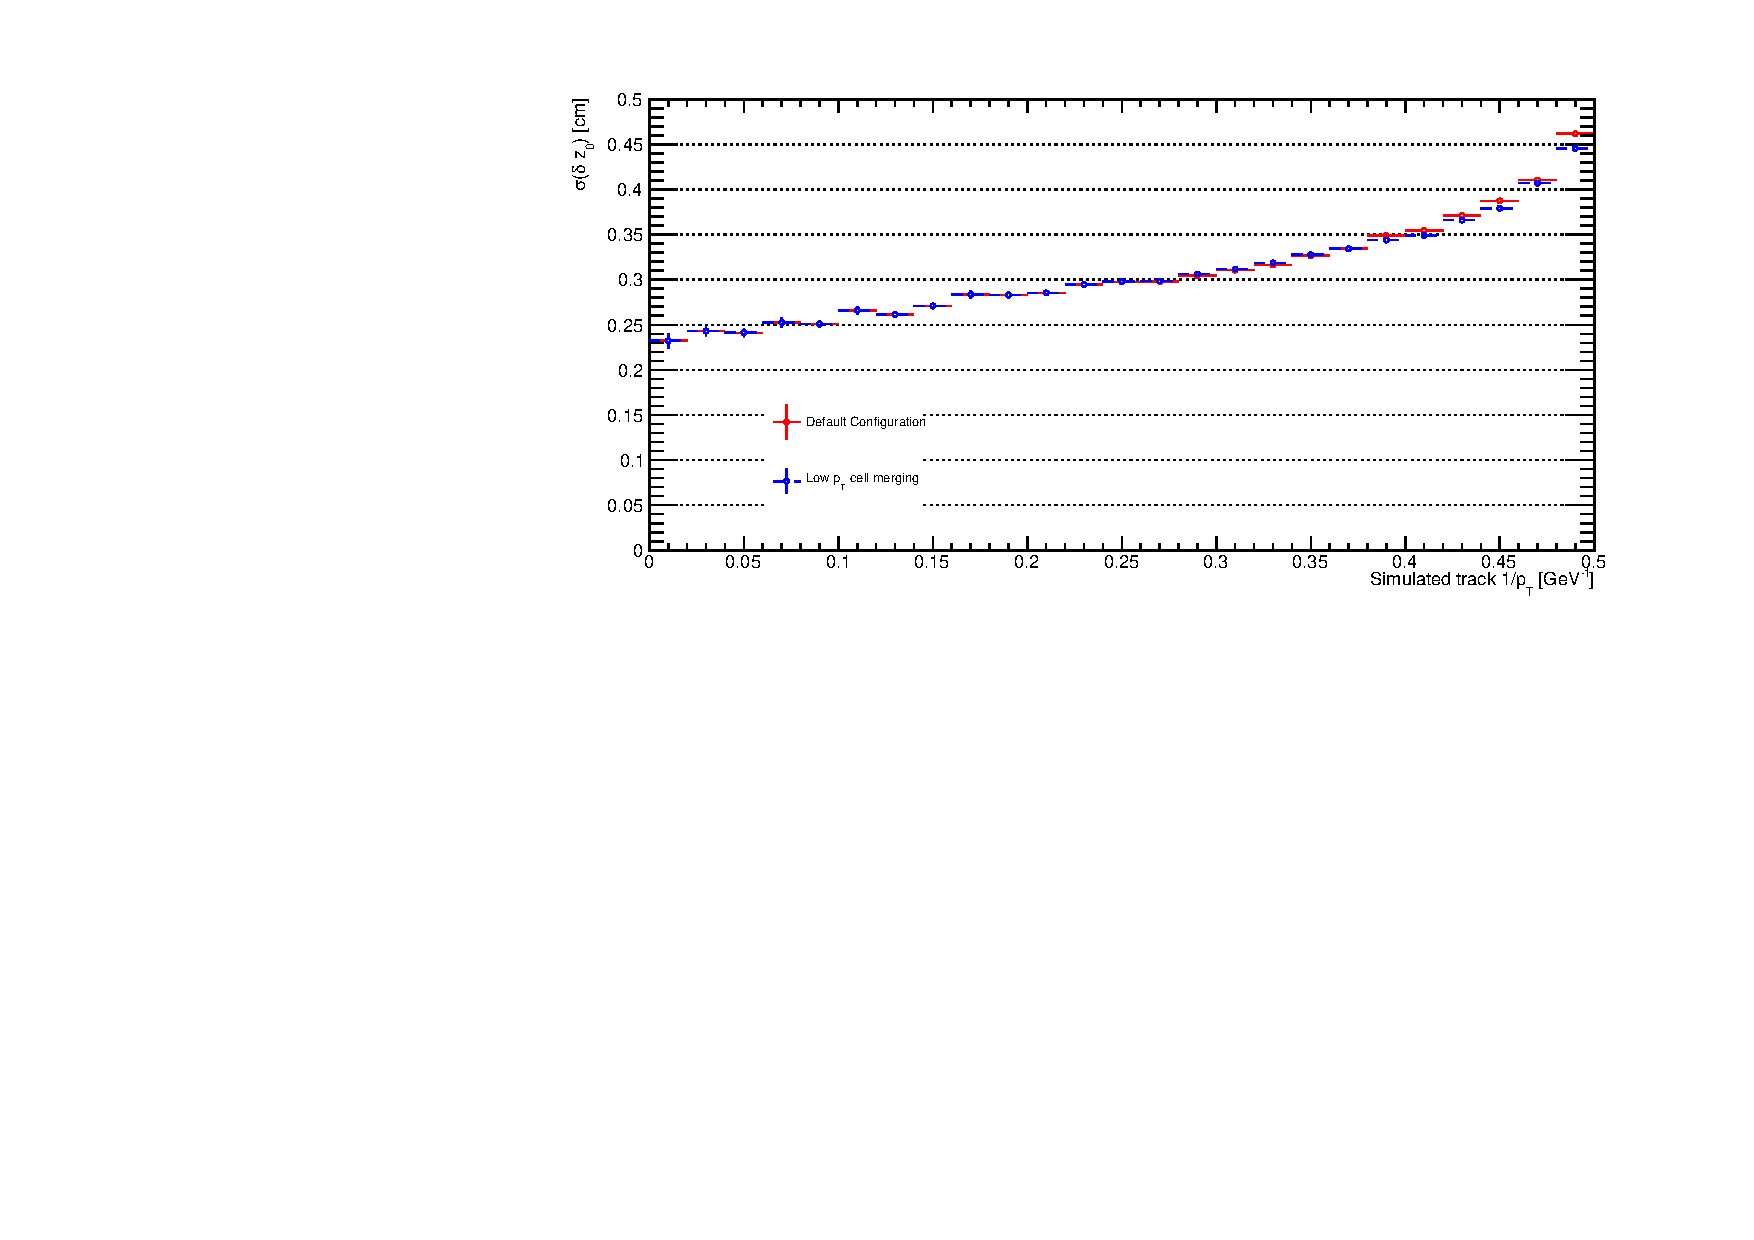
\includegraphics[width=0.49\textwidth]{figs/tk-upgrade/results-lowPtTracking/z0ResVsInvPtFlatGeometry_5000.pdf}
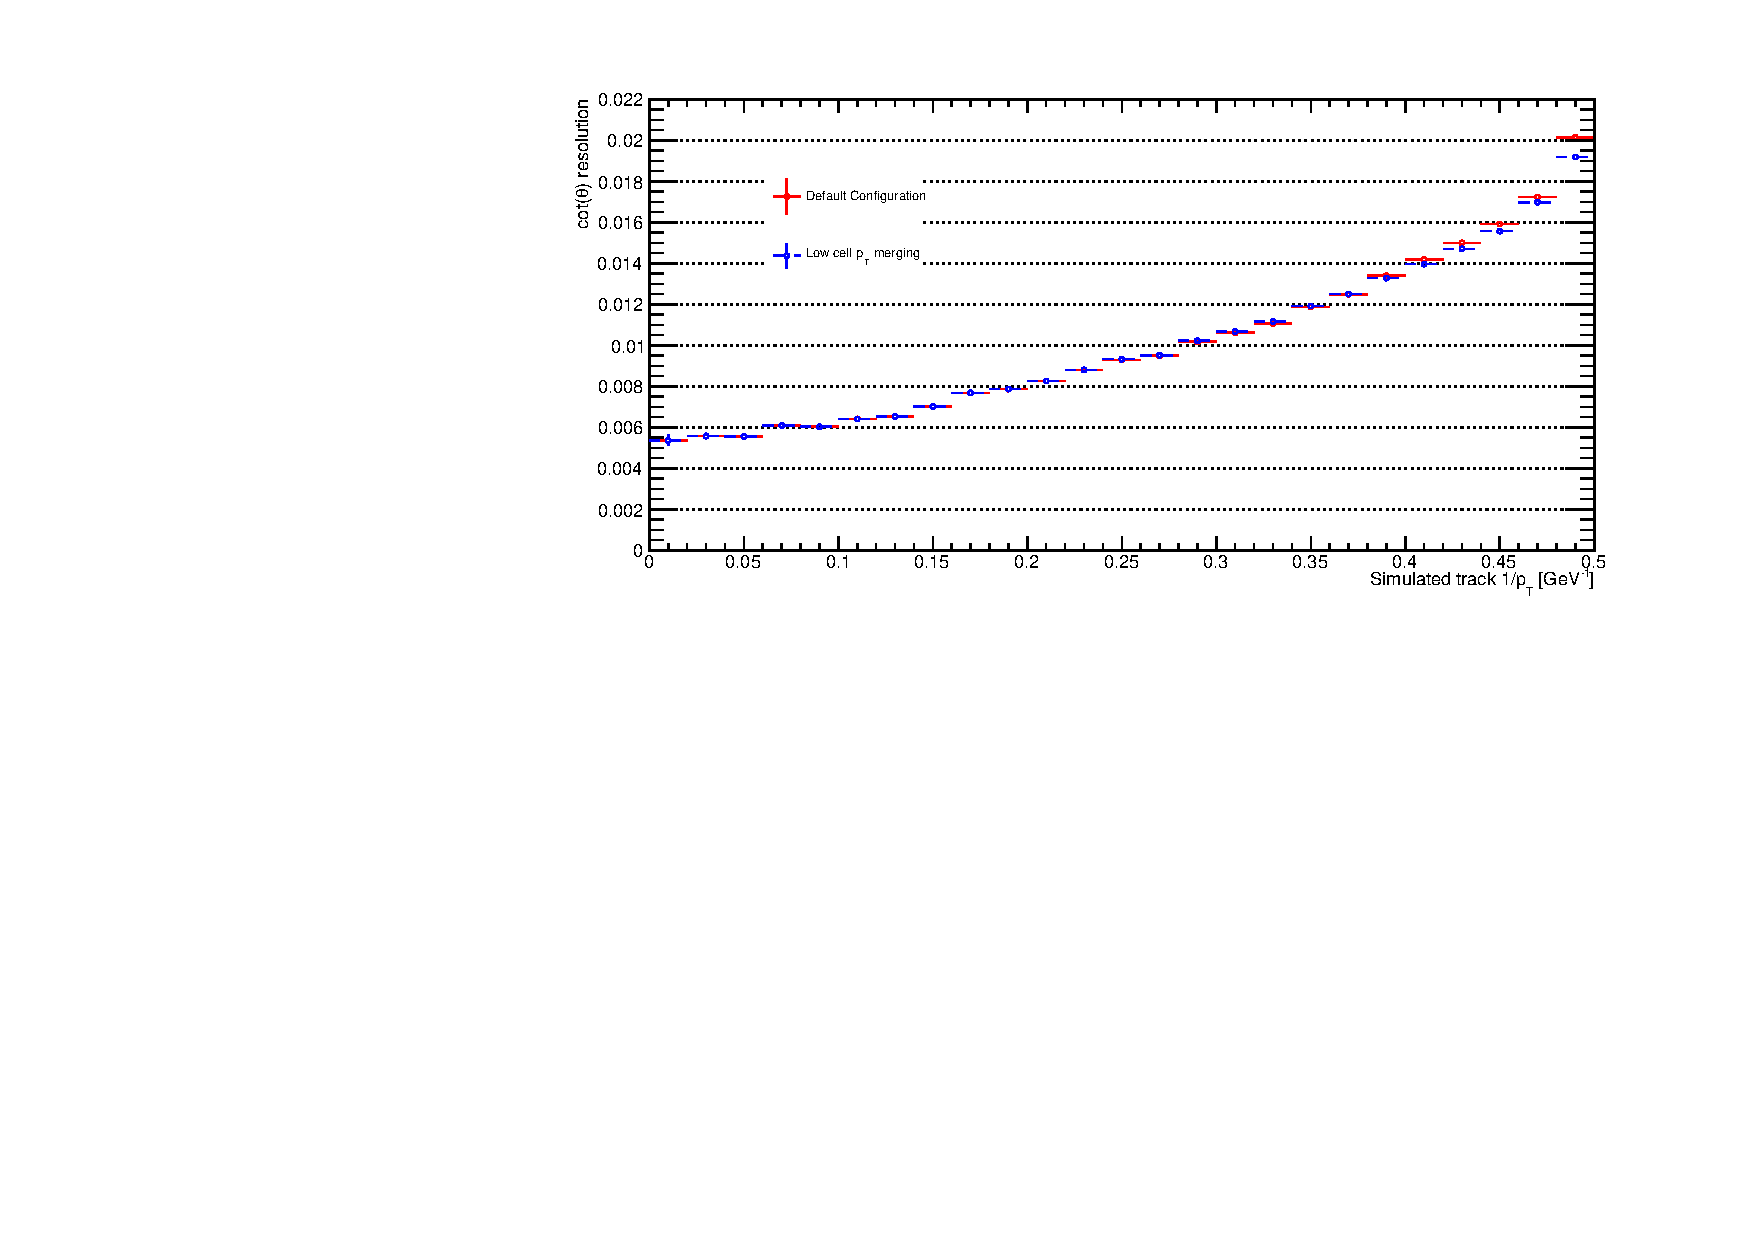
\includegraphics[width=0.49\textwidth]{figs/tk-upgrade/results-lowPtTracking/cotThetaResVsInvPtFlatGeometry_5000.pdf}
\caption{
The \pt resolution, $\phi$ resolution, $z_{0}$ resolution and cot$\theta$ resolution measured for both the default configuration where only the number of \HT \qpt columns have been increased (red) and after the \HT and \KF optimisations have been applied (blue) for primary reconstructed tracks in simulated \ttbar events at a <PU> of 200 for tracks with $\pt > 2\GeVc$.
\editComment{Make plots bigger!}
}
\label{fig:htHelixParametersResVsInvPt}
\end{figure}

\subsubsection{Kalman Filter Optimisation}\label{subsubsec:lowPtOptKF}
Incorporation of \MS into the \KF involved including a \emph{process noise} term, namely the variance of the multiple scattering angles, to the \emph{measurement noise} (\ie measurement error) term already present in the \KF covariance matrix.
In this updated form, the \KF now can consider stubs which are compatible with those that have undergone \MS, allowing tracks with previously discarded stubs to be reconstructed and the resultant more accurate $\chi^{2}$ values which can be used to better discriminate against fake track states.

For small deflection angles and relativistic particles, $\sigma_{\theta}$ for a each layer is given by~\cite{Lynch:1990sq}~:

\begin{equation}
\sigma_{\theta} = \frac{13.6\MeV}{\beta c p} q \sqrt{\frac{x}{X_{0}}} [1 + 0.088 \log_{10}{\frac{x}{X_{0}}}]  \;
\label{eq:scatter1}
\end{equation}

where, the momentum, velocity, electrical charge of the incident particle and thickness of the scattering medium in radiation lengths are given by $p$, $\beta c$, $q$ and $\frac{x}{X_{0}}$ respectively and the result being good to better than 11\%.

With the particles involved having relativistic velocities (\ie $\beta c \cong 1$) and scattering in the r-z plane ignored as the impact of multiple scattering is considerably smaller hit position resolution in r-z, the multiple scattering contribution in the \rphi plane can be expressed as:

\begin{equation}
\sigma_{\theta} = \frac{k}{\pT}
\label{eq:scatter2}
\end{equation}

where $k$ is a coefficient.

From the simplified form of Equation~(\ref{eq:scatter2}), two alternative forms of the coefficient $k$, which should require minimal resources and latency, were investigated:

\begin{itemize}
\item \textbf{constant coefficient - } a constant coefficient of the order of the average anticipated scattering angle is used as the anticipated typical scattering angle for $2-3\GeV$ tracks is of the order of a milliradian.
\item \textbf{layer dependent coefficient -} the coefficient used is a function of the layer ID (\ie which layer the stub is found) in order to take into account the impact of repeated scattering from passing through multiple layers increasing the uncertainty associated of the hit position.
\end{itemize}

The initial layer dependent coefficients were obtained through experimentally determining in simulation the \MS  contribution to the observed variance in $\phi$.
Both these initial layer dependent coefficients and the initial constant coefficient of a milliradian were subsequently further optimised in order to recover as much tracking efficiency as  possible.
Similarly, the \KF state $\chi^{2}$ cuts for both approaches were also tuned in order to reject the optimal number of fake and duplicate tracks without compromising on tracking efficiency.

During the comparative studies of these two approaches, as shown in figure~\ref{fig:2GeVfracDups} it was observed that following the \DR stage that the fraction of duplications present increases above circa $3\GeV$ in contrast to the trend of the fraction of duplicates decreasing as \pT decreases.
As this feature is present following the \HT stage, without any further stage being run, this implies that the \HT produces more duplicates at low \pT in the full precision cells.
As the fraction of duplicate tracks produced where decreased precision \HT cells are used is well controlled, the \pT threshold for the $2 \times 2$ merging of \HT cells was increased from $2.7\GeV$ to $3.5\GeV$.
While an increase in the duplicate rate is observed between $3.2\GeV$ and $5\GeV$ in figure~\ref{fig:2GeVfracDups}, a decreased number of duplicates were produced below $3.5\GeV$ which lead to an overall reduction in the number of duplicates produced of circa 2.8\%.

The increased \pT threshold for \HT cell merging also had the additional benefit of recovering an additional 0.2\% of the tracks which were previously lost to \MS.
Consequently, this change was adopted by the project and all the results presented below for the two \MS coefficient forms were produced using this increased threshold. 

\begin{figure}[tbp]
\centering
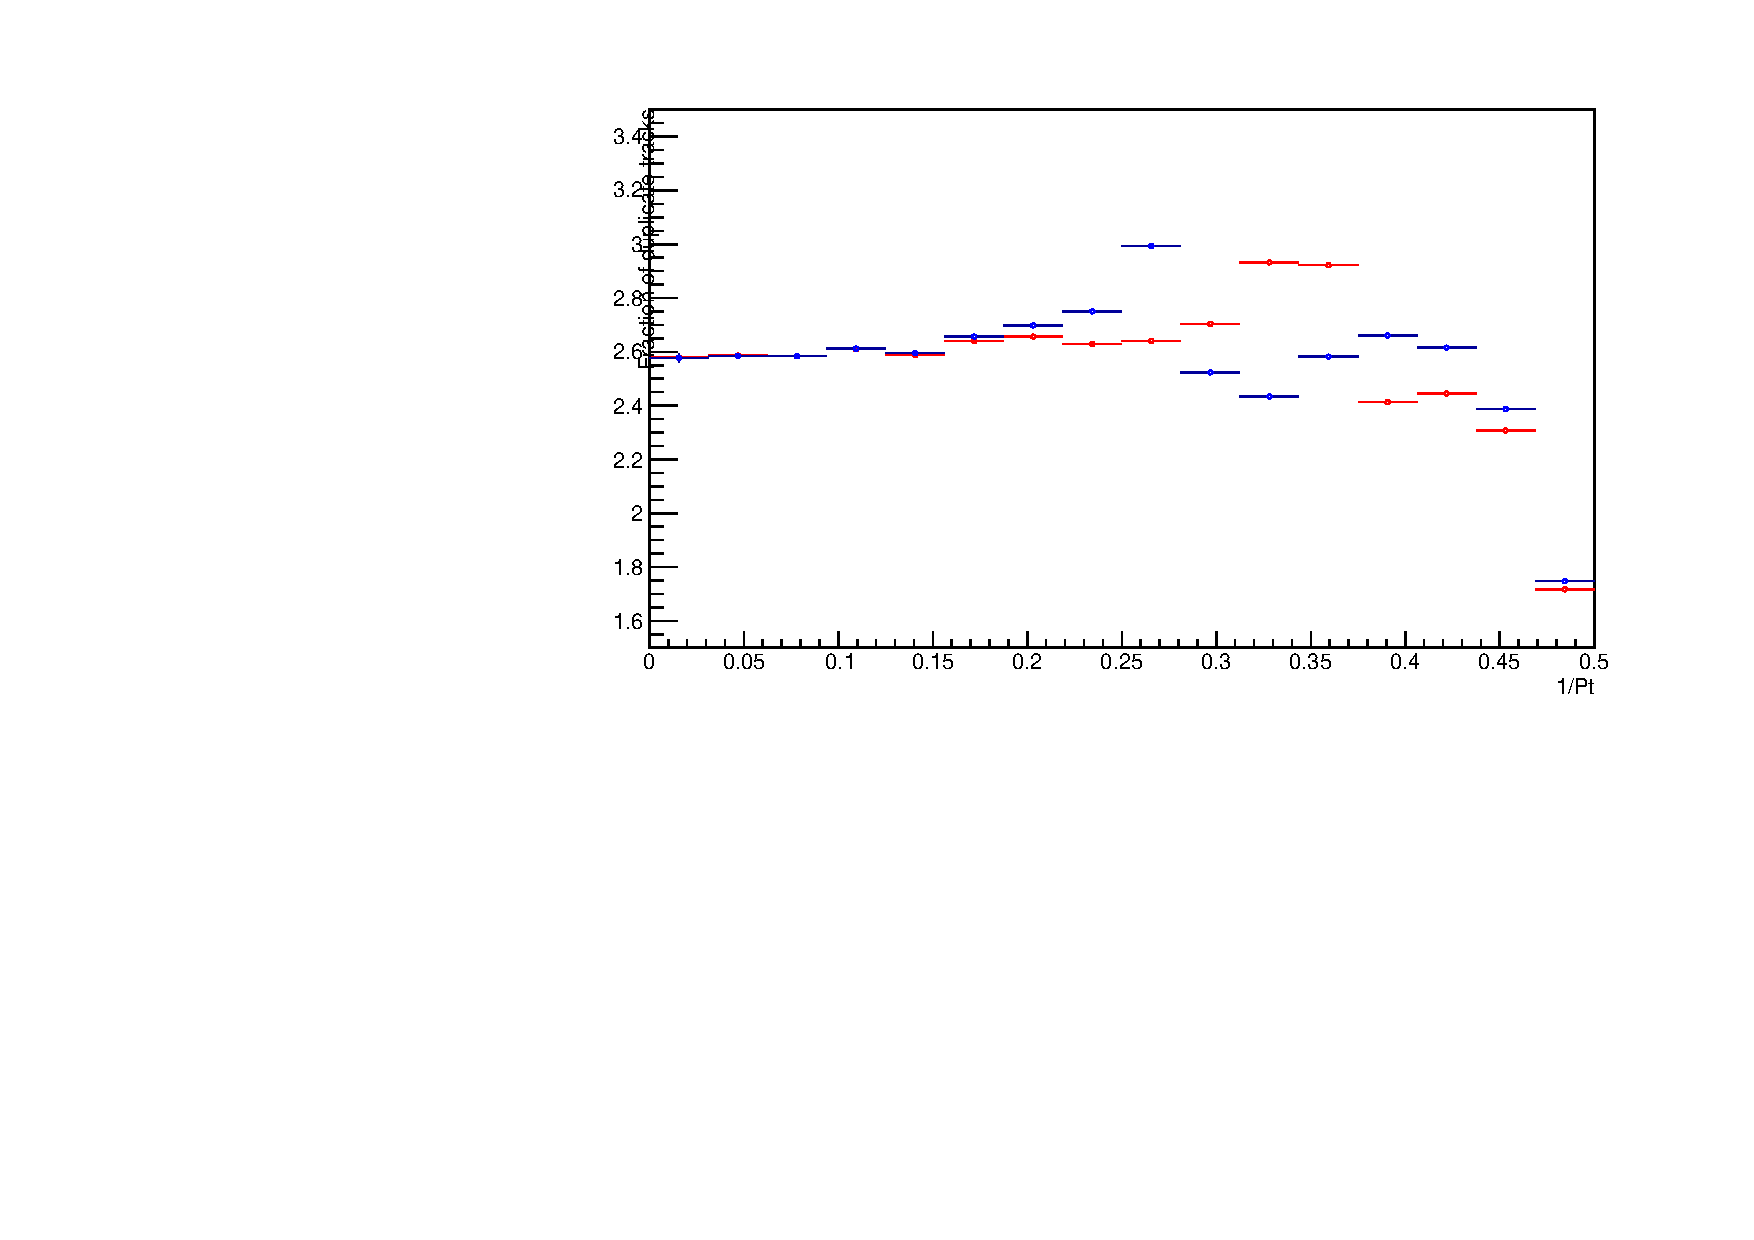
\includegraphics[width=0.49\textwidth]{figs/tk-upgrade/results-lowPtTracking/htFracDuplicatesVsInvPtTiltedGeometry_5000.pdf}
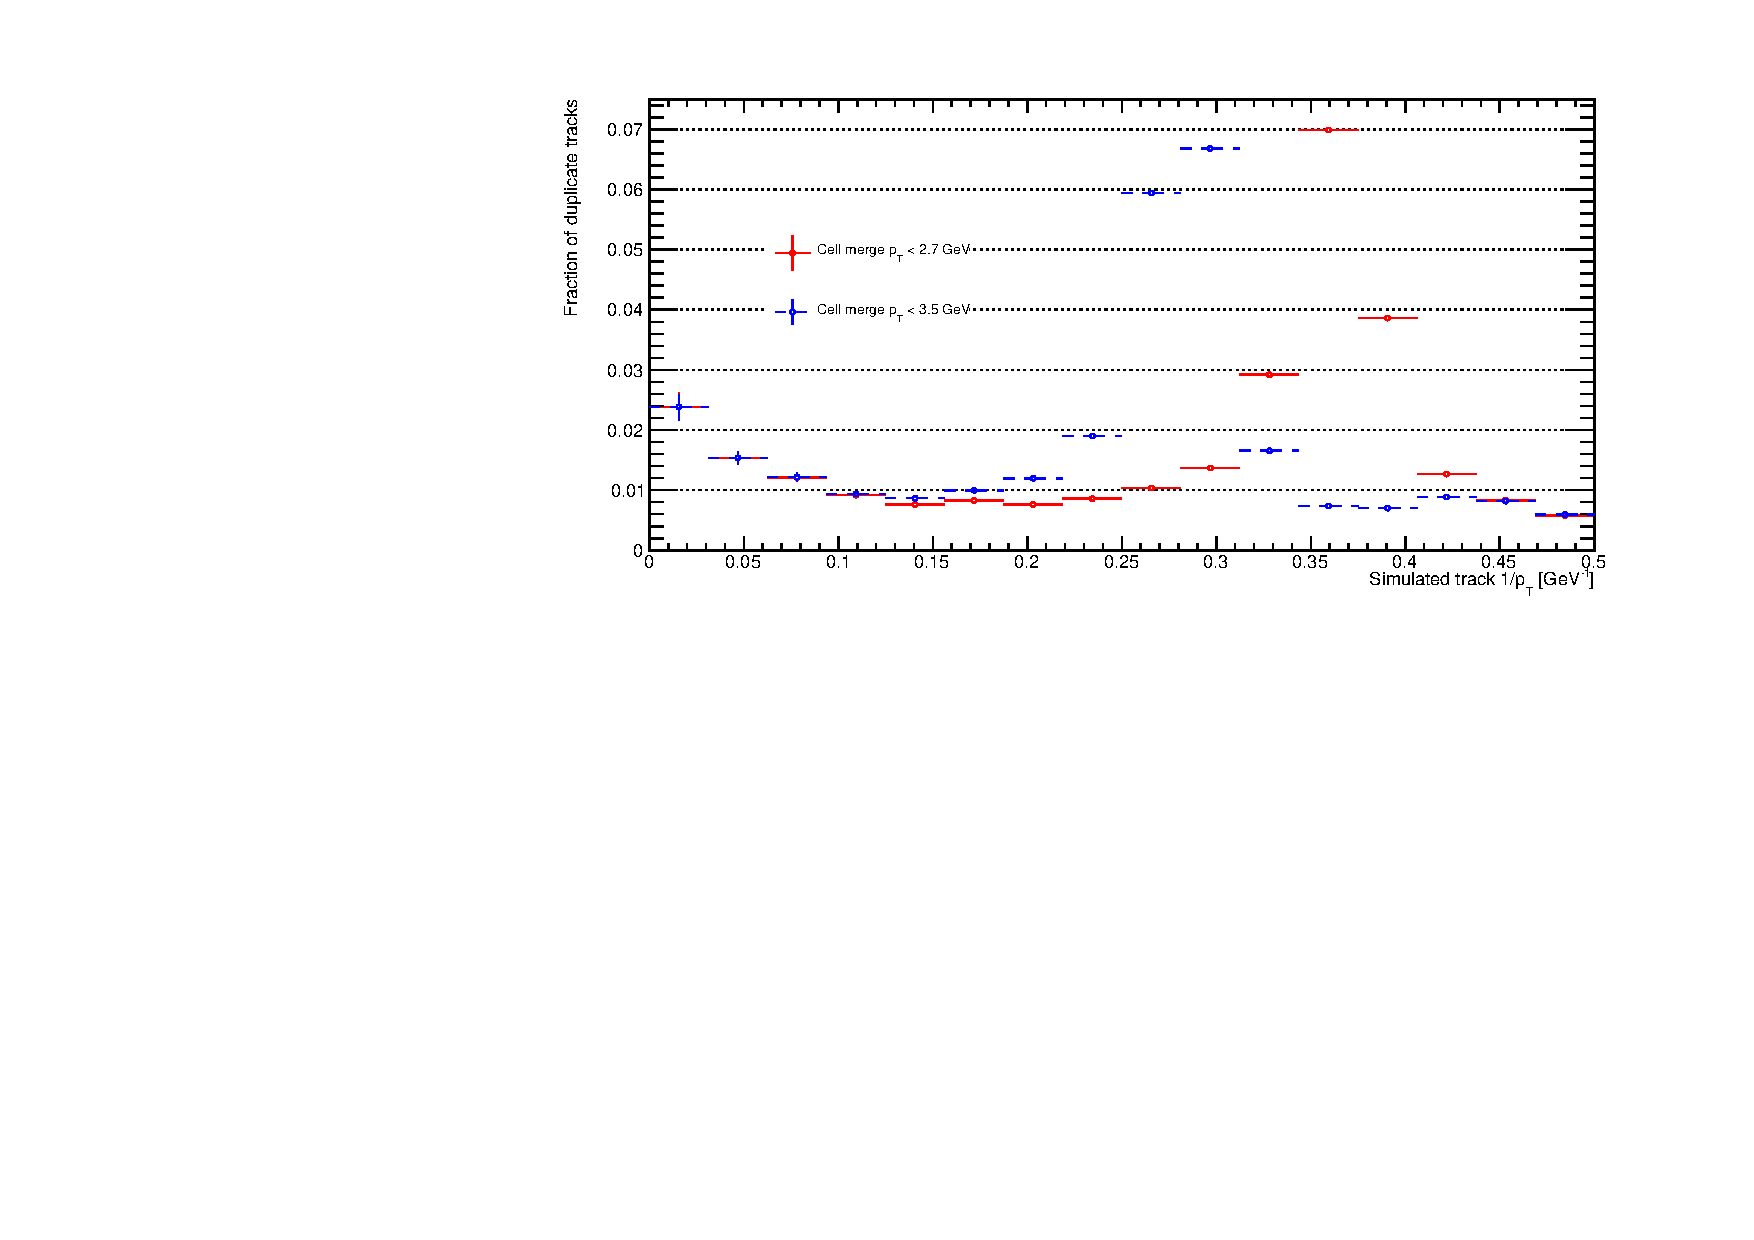
\includegraphics[width=0.49\textwidth]{figs/tk-upgrade/results-lowPtTracking/kfFracDuplicatesVsInvPtTiltedGeometry_5000.pdf}
\caption{The fraction of genuine tracks with duplicates as a function of $\frac{1}{\pT}$ following reconstruction by the \HT (left) and fitting and filtering by the \KF and \DR (right) for where the \HT cell merging \pT threshold is set to 2.7\GeV (red) and 3.5\GeV (blue). 
The constant coefficient for the \MS contribution was used for these \KF results.
\editComment{Resize plots!}
}
\label{fig:2GeVfracDups}
\end{figure}

\begin{figure}[tbp]
\centering
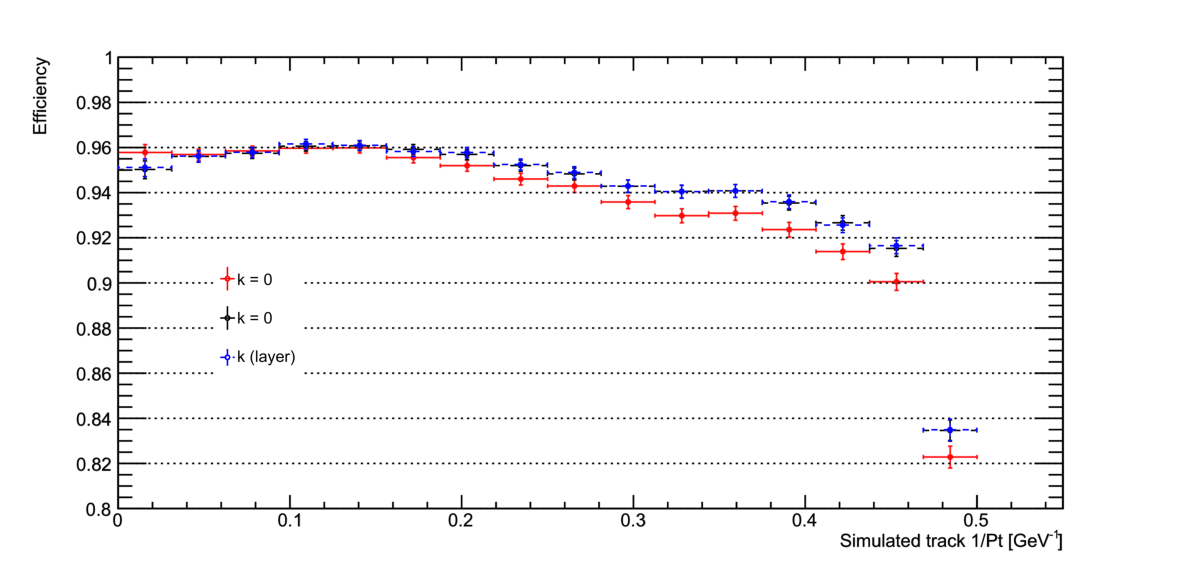
\includegraphics[width=\textwidth]{figs/tk-upgrade/results-lowPtTracking/kfTrackingEffVsInvPtTiltedGeometry_5000.pdf}
%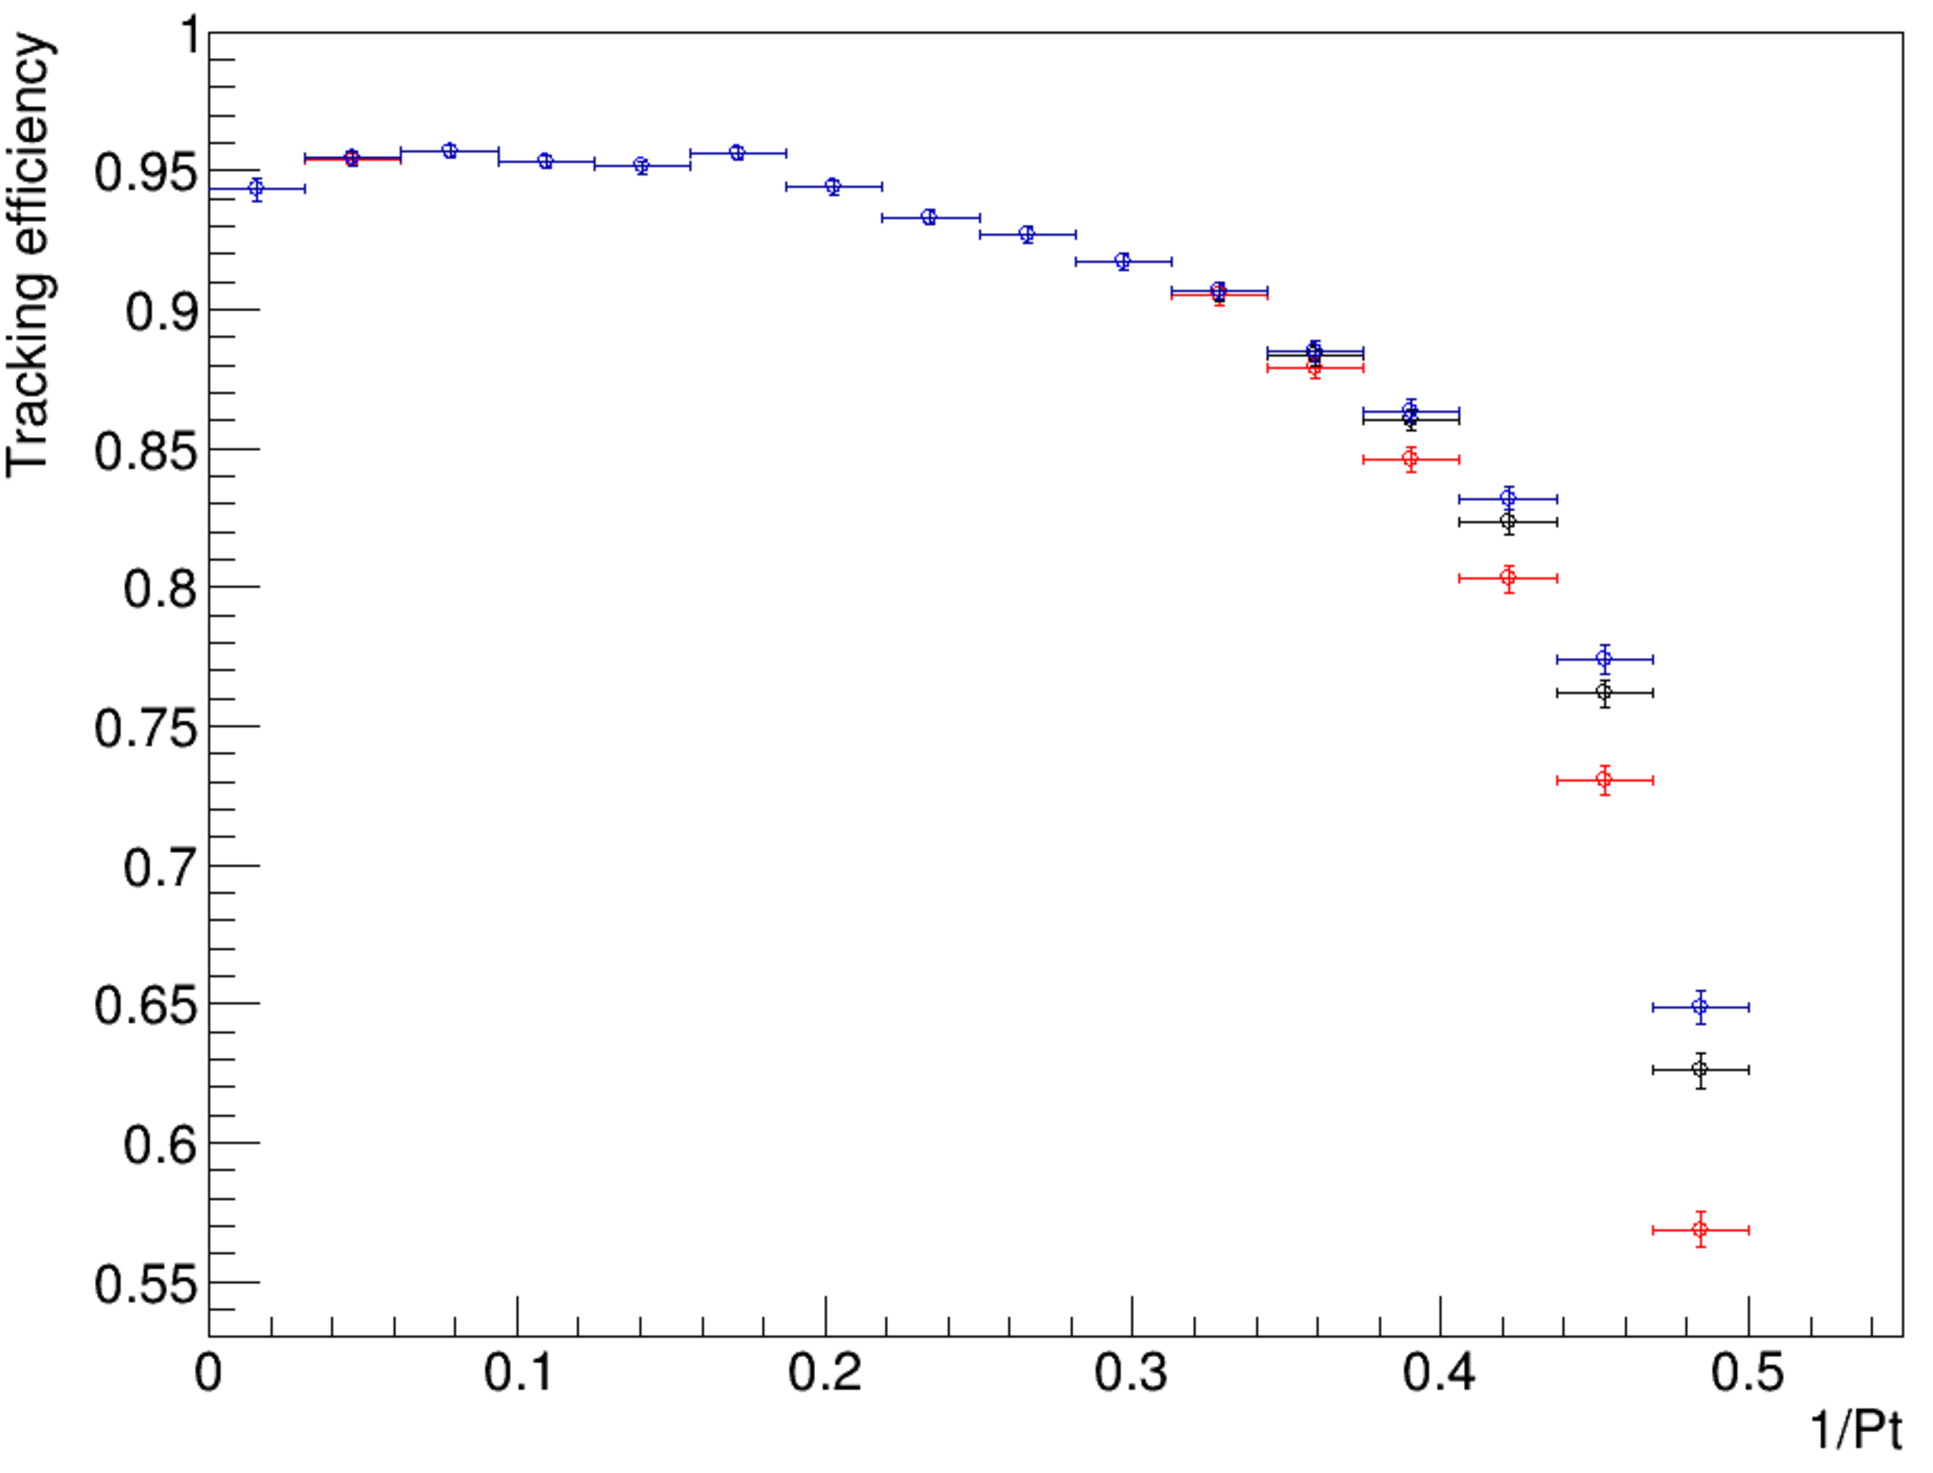
\includegraphics[width=\textwidth]{figs/tk-upgrade/results-lowPtTracking/kfTrackingEffVsInvPtFlatGeometry_5000.pdf}
\caption{Plots showing tracking efficiency as a function of $\frac{1}{\pT}$ for \ttbar events at a <PU> of 200 after the full chain has been run, where the \KF has not been modified to take \MS into account (red), a constant coefficient for \MS is used (black) and a layer dependent coefficient for \MS is used (blue).
}
\label{fig:2GeVTiltEff}	
\end{figure}

Figure~\ref{fig:2GeVTiltEff} shows how the tracking efficiency for the whole chain improves when \MS is accounted for in the \KF.
The similar performance observed between the two coefficients in figure~\ref{fig:2GeVTiltEff} and Table~\ref{tab:trackFindingPerformance2GeVKF} is due the amount of material traversed by a track not being constant for a single layer as the amount of material contributions in both the tracker and the prior contributions from the Inner Tracker, between the Inner and Outer Trackers and services varies as a function of $\eta$~\cite{P2TrackerTDR}.

Table~\ref{tab:trackFindingPerformance2GeVKF} also shows that compared to just the \HT optimisations alone, for both \MS coefficients, the \KF is more capable at rejecting incorrectly reconstructed tracks by up to an additional 3-4\%.
In contrast, the duplicate increases for both coefficients by 3-5\% for the full chain, with the increase in duplicates occurring between $3.2\GeV$ and $5\GeV$, as shown in figure~\ref{fig:2GeVfracDups}, near the $3.5\GeV$ threshold for merging adjacent \HT cells.
At the time of writing this chapter, it is not understood how incorporating \MS into the \KF causes this, but it is suspected to be related to the use of the reduced precision of \HT cells.
\editComment{It is hoped that by the time of submission, someone (Ian ... ?) will have figured this out.}
%Tracks with \pt approaching the \pt threshold at which reduced precision of \HT cells are used are have the potential to be built out of both stubs from both the full and reduced precision \HT cells.

\begin{table}[htbp]
\topcaption {Track finding performance on simulated \ttbar events at a <PU> of 200, after the full demonstrator chain for the three differing \KF configurations where \MS is not considered ($k = 0$), a constant \MS coefficient (const $k$) is used and a layer dependent \MS coefficient ($k(layer)$)is used. 
The track finding efficiencies following each stage are given using the efficiency definitions given in Section~\ref{subsec:helixParameter}, along with the mean number of tracks and the fraction of those tracks which are either fake or duplicate tracks.
\editComment{Fix table size!.}
}
\label{tab:trackFindingPerformance2GeVKF}
\centering
 \resizebox{\textwidth}{!}{
\begin{tabular}{ccccc}
   \hline
   \bf{Scattering coefficient} & \bf{Efficiency [\%]} & \bf{Mean \# of tracks} & \bf{Fakes [\%]} & \bf{Duplicates [\%]}  \\
   \hline
%     & \bf{HT}     &  96.2 & 752.0 & 28.2 & 47.3 \\  
   $k = 0$  & 93.6 & 216.0 & 13.3 & 9.4 \\      
   \hline
   const $k$ & 94.2 & 216.3 & 10.3 & 11.2 \\      
   \hline
    $k(layer)$ & 94.2 & 222.1 & 10.8 & 12.3 \\  
   \hline
   
\end{tabular}}
\end{table}

Figure~\ref{fig:kfHelixParametersResVsInvPt} shows the resolutions of the track parameters as a function of transverse momentum in simulation for tracks originating from the primary interaction in \ttbar events at a <PU> of 200 for both \MS coefficients considered as well as when \MS is not accounted for at all.
The resolutions of both \MS coefficients are superior across all \pt to when \MS is not considered at all, with the constant \MS coefficient typically providing more slightly more precise measurements than the layer dependent coefficient.  
As expected, lower transverse momentum tracks experience the greatest improvements given that \MS dominates at lower transverse momenta.
For both coefficients however, the \pt resolution in the range $ 3.8 \GeV < \pt < 5.5\GeVc$ is worse than when \MS is not considered.
At the time of writing, this observation is still being investigated, but is suspected, like the increased duplicate rate in the same \pT range, to be related to the reduced precision of \HT cells.

\begin{figure}[htb]
\centering
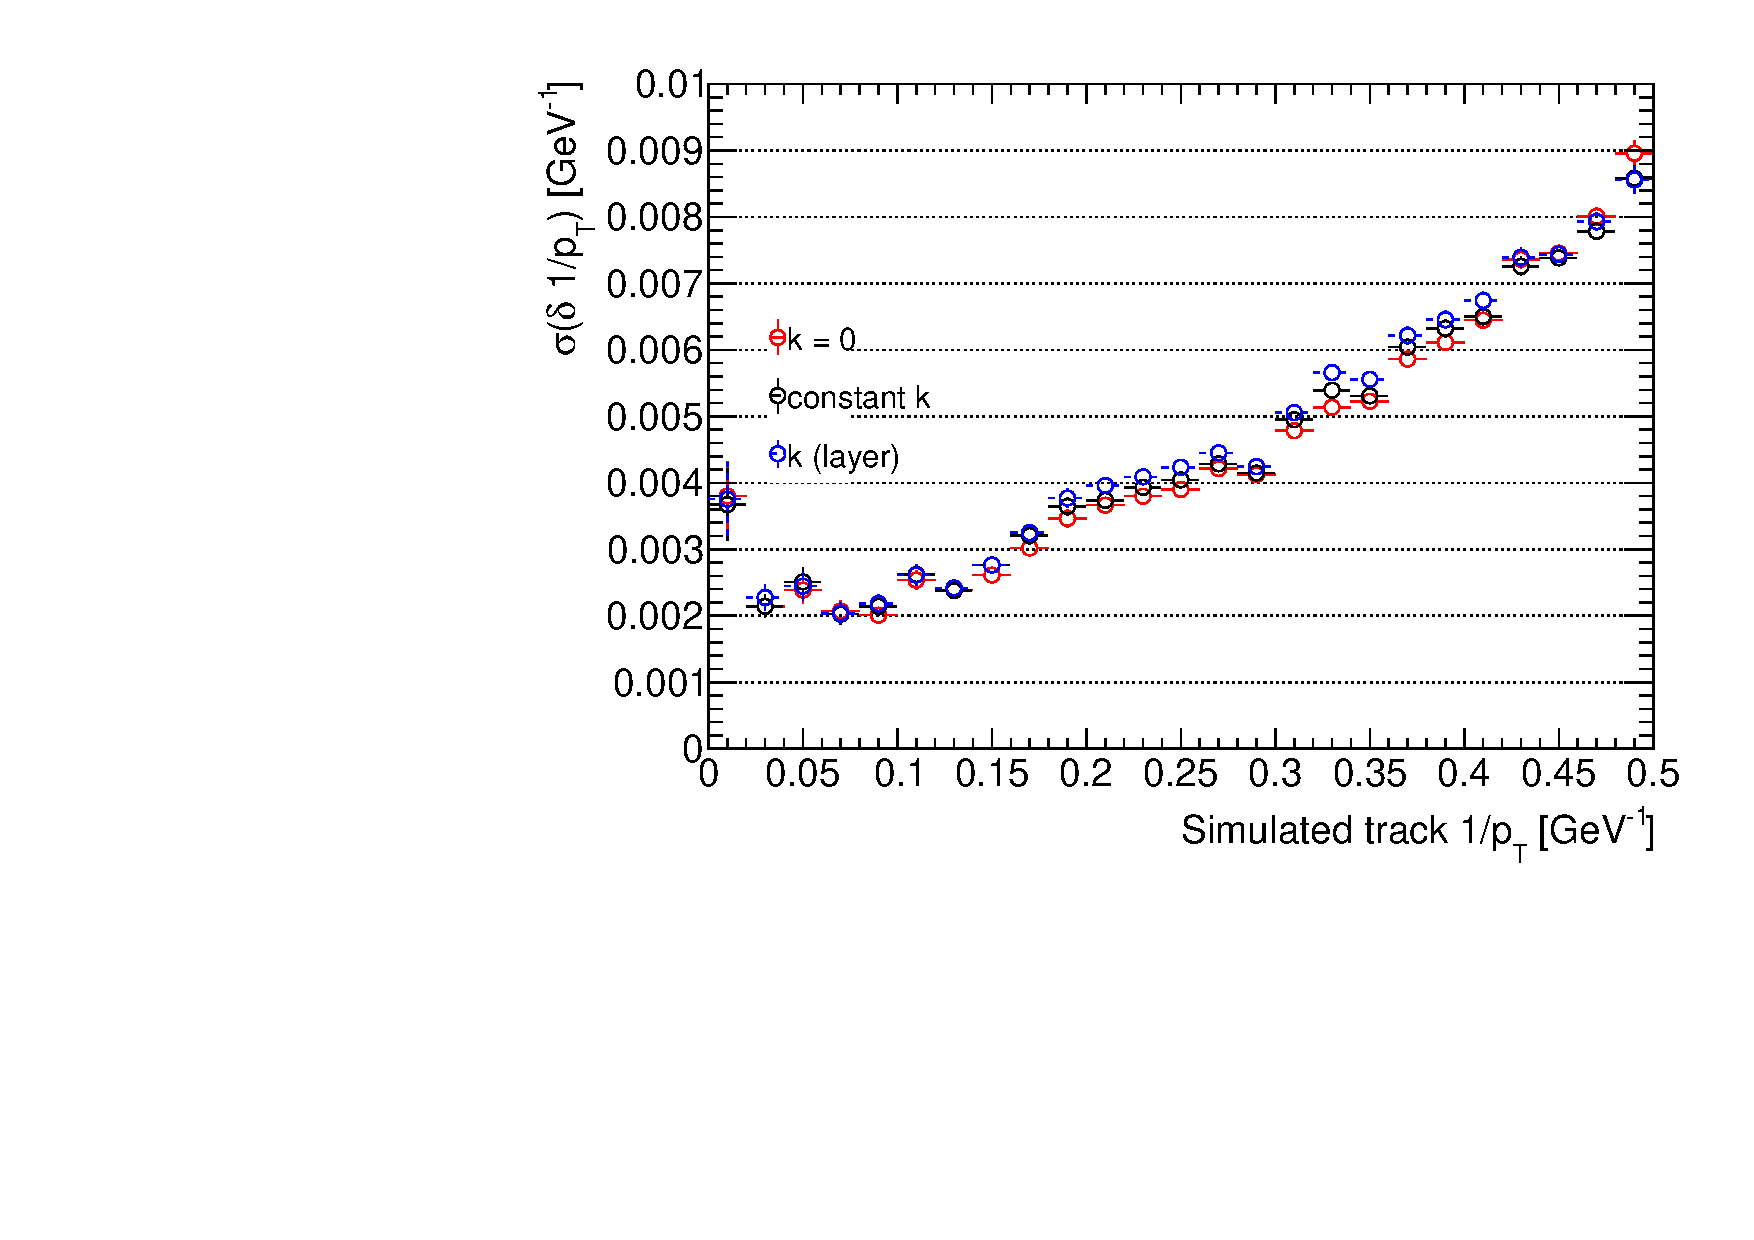
\includegraphics[width=0.49\textwidth]{figs/tk-upgrade/results-lowPtTracking/qOverPtResVsInvPtTiltedGeometry_5000.pdf}
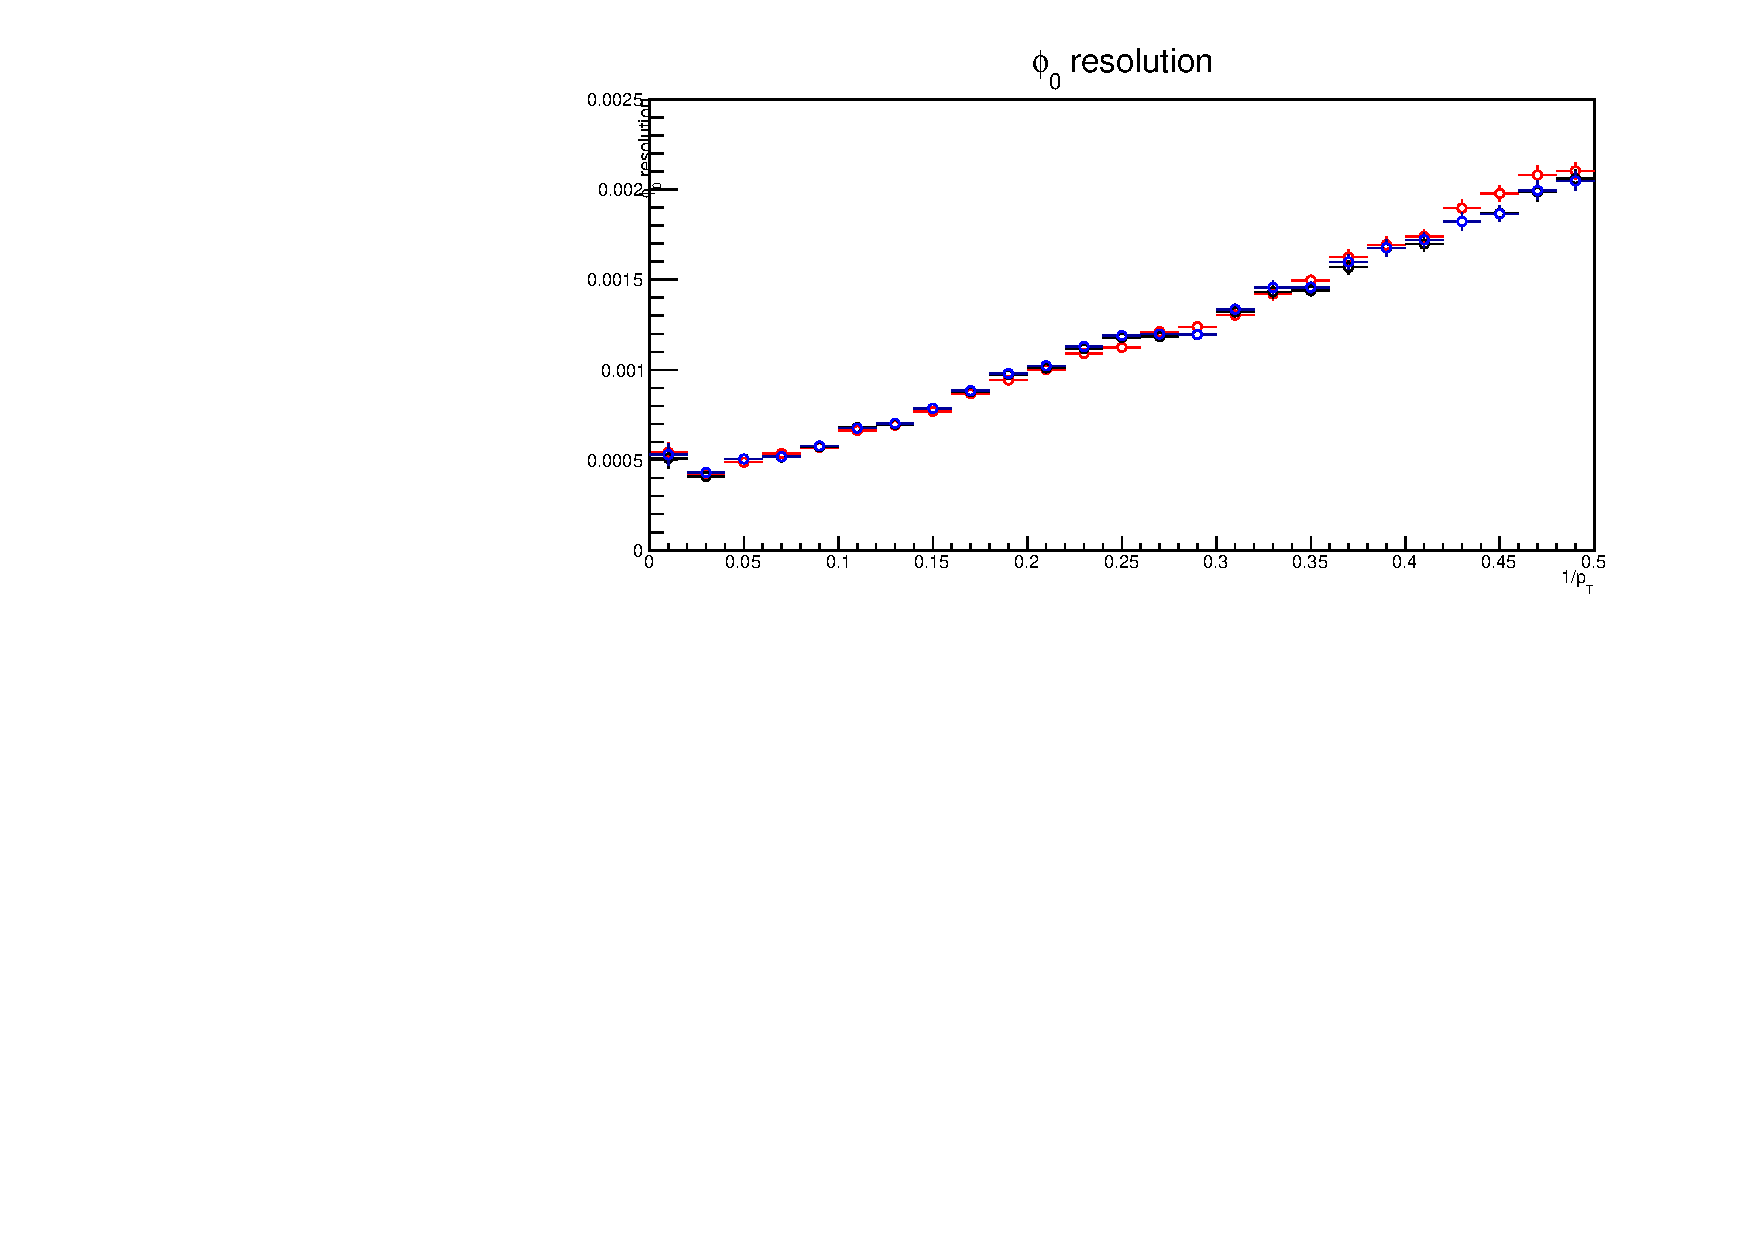
\includegraphics[width=0.49\textwidth]{figs/tk-upgrade/results-lowPtTracking/phi0ResVsInvPtTiltedGeometry_5000.pdf}
\\
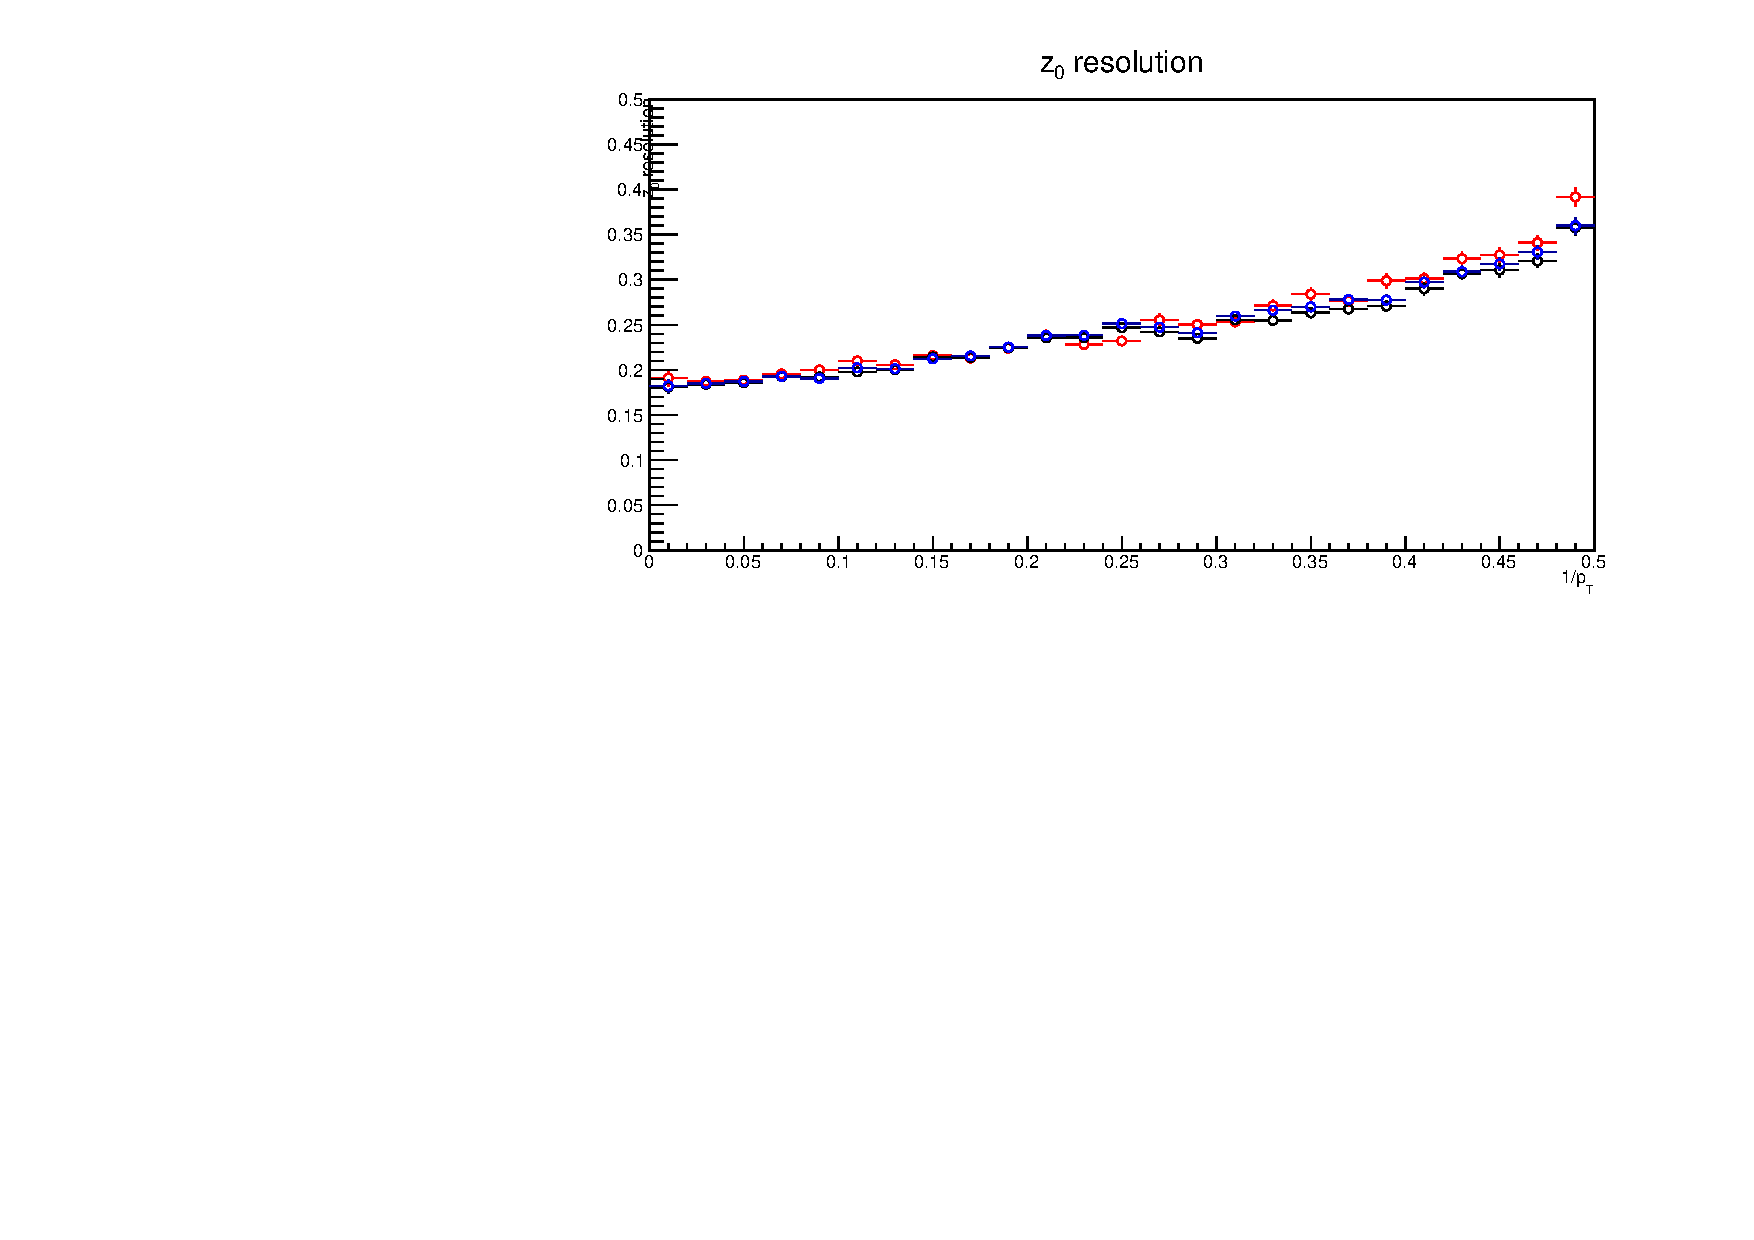
\includegraphics[width=0.49\textwidth]{figs/tk-upgrade/results-lowPtTracking/z0ResVsInvPtTiltedGeometry_5000.pdf}
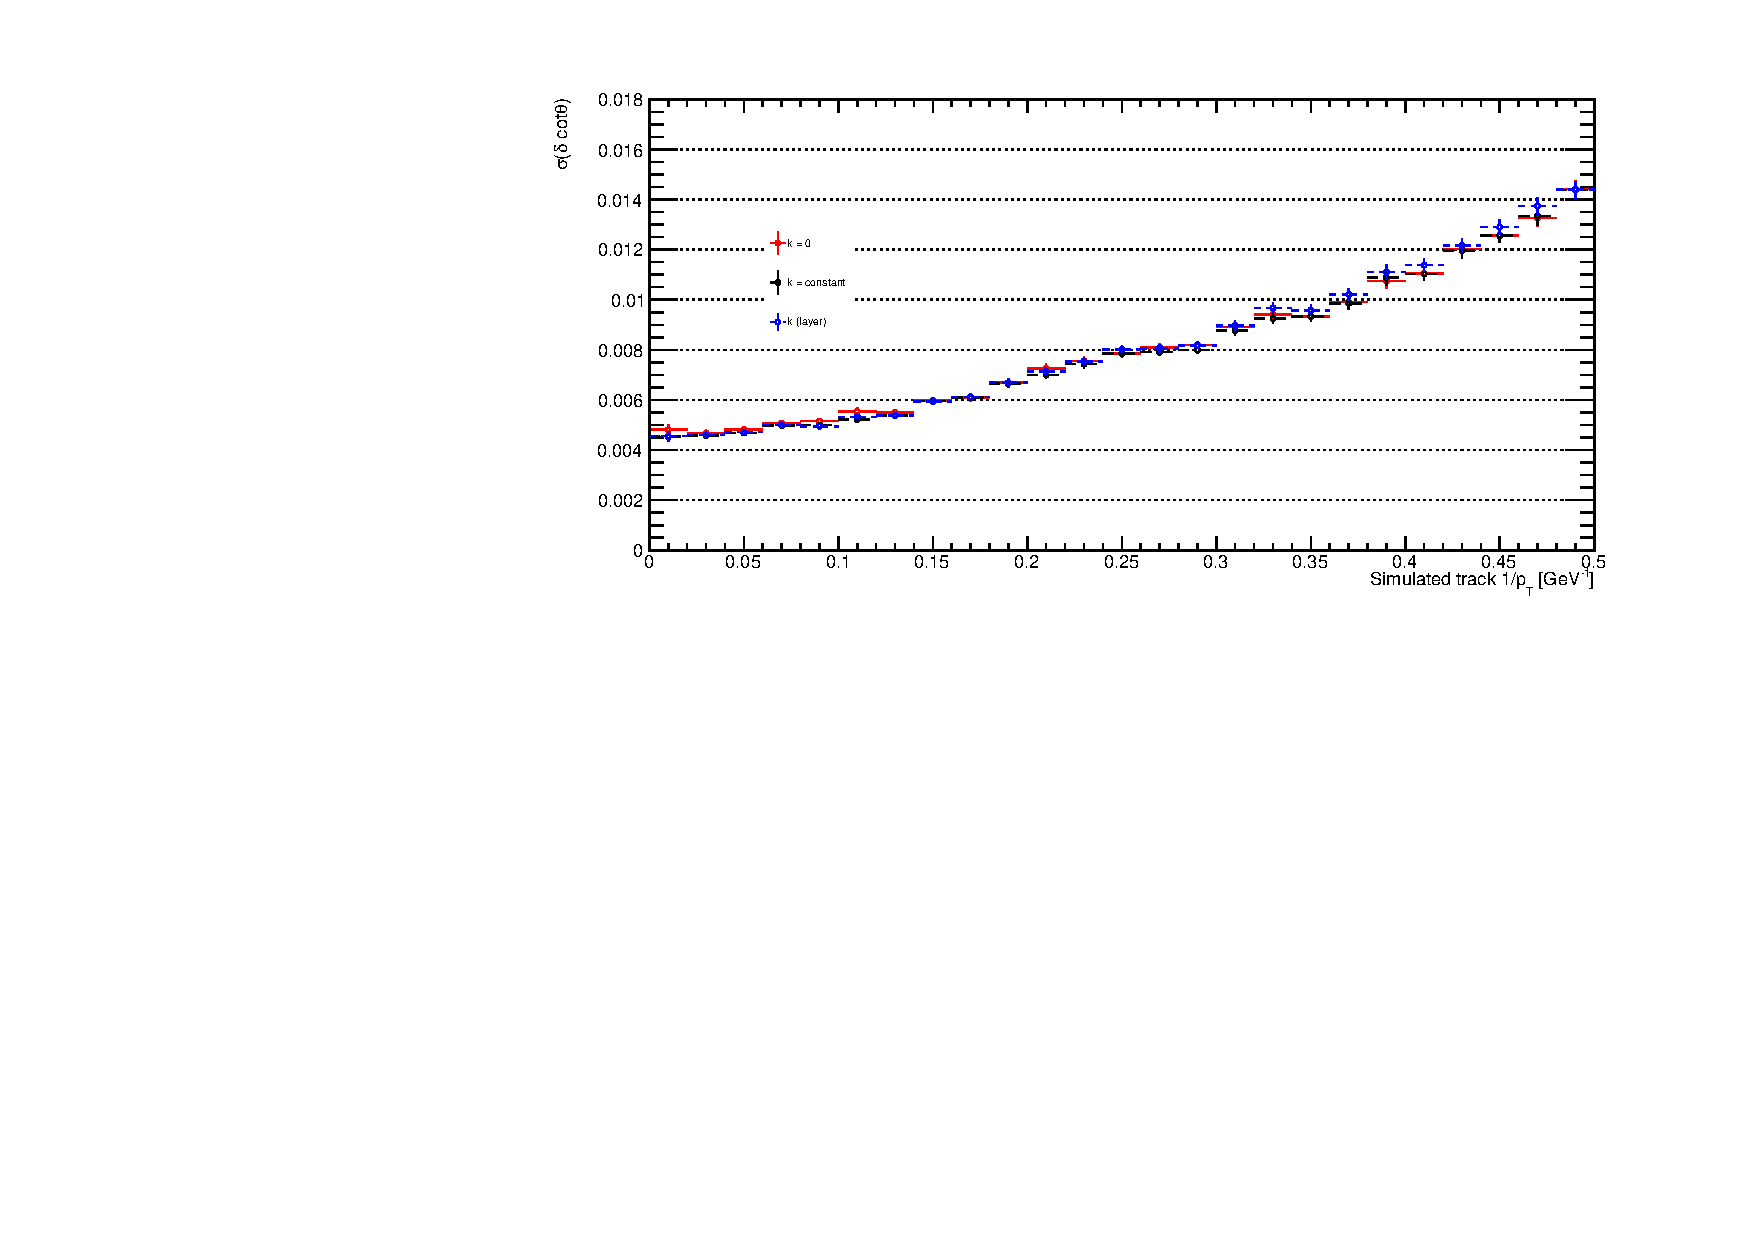
\includegraphics[width=0.49\textwidth]{figs/tk-upgrade/results-lowPtTracking/cotThetaResVsInvPtTiltedGeometry_5000.pdf}
\caption{\pt resolution, $\phi$ resolution, $z_{0}$ resolution and cot$\theta$ resolution measured for primary reconstructed tracks in simulated \ttbar events at a <PU> of 200 for when multiple scattering isn't considered by the \KF (red), when a constant \MS coefficient is used (black) and when a layer dependent coefficient is used (blue).
}
\label{fig:kfHelixParametersResVsInvPt}
\end{figure}

\subsubsection{Conclusions}\label{subsubsec:2GevConclusions}
After investigating modifications to the \HT and \KF algorithms to improve upon the default performance obtained for track finding and fitting of low \pT ($< 3\GeV$) tracks.
The decreased precision \HT cells enables the recovery of some of the tracks previously lost due to \MS, and the inclusion of a process noise term allows the \KF to take the impact of \MS into account, as shown in Figure~\ref{fig:2GeVTiltChi2Ndf} where the $\frac{\chi^{2}}{ndf}$ of the matched tracks fitted has not only decreased at high \pT where \MS dominates, but also the smaller effects experienced at higher \pT.
Both formulations of the \MS term provide considerable improvement in the track reconstruction efficiency and helix parameter resolutions obtained.
The lack of any noticeable improvement between using a constant \MS coefficient and one which is a function of the number of layers traversed, is a consequence of knowing which layer a hit belongs to not being a good descriptor of the total amount of material at that point.
As the amount of material traversed will depend on the trajectory of the charged particle, such a coefficient would likely have to be a function of \pt and $\eta$.

\begin{figure}[tbp]
\centering
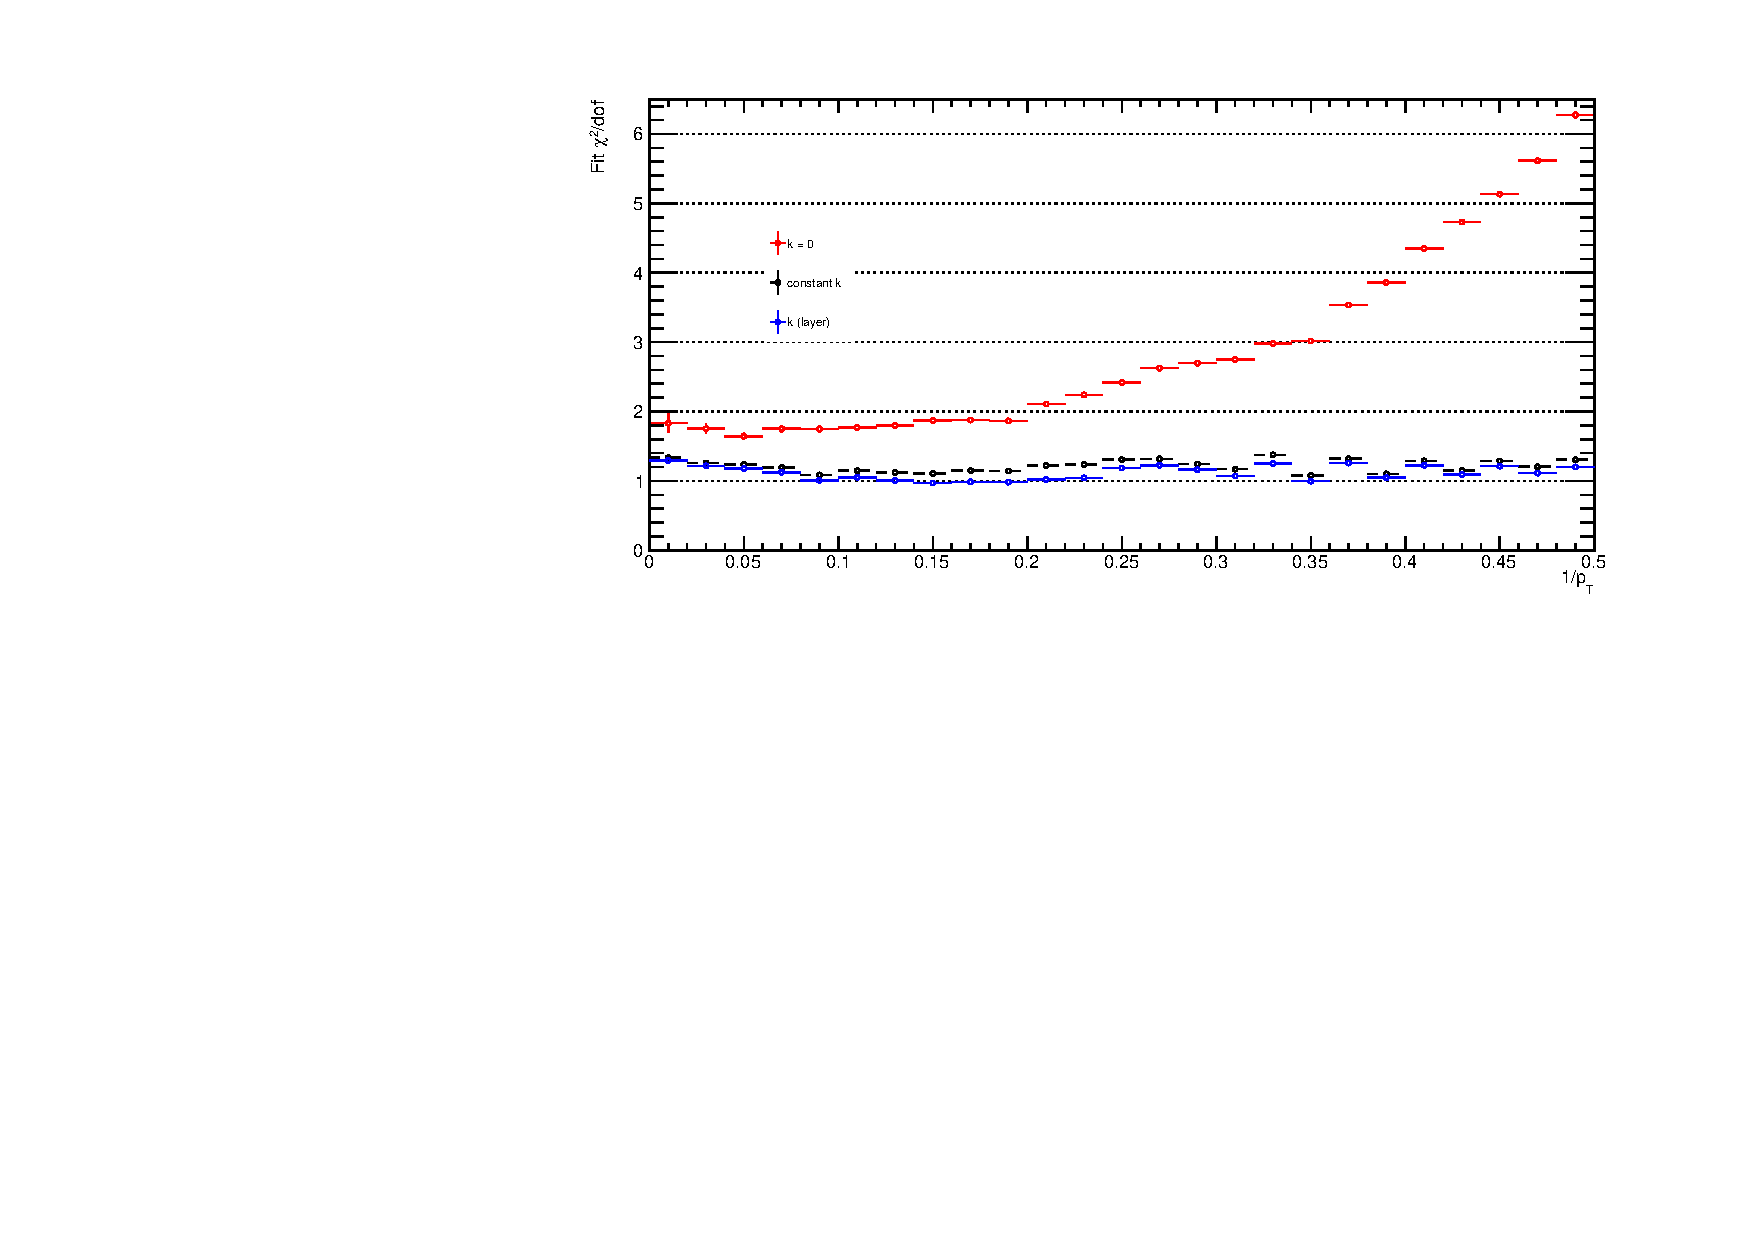
\includegraphics[width=\textwidth]{figs/tk-upgrade/results-lowPtTracking/kfChi2NdfVsInvPtTiltedGeometry_5000.pdf}
\caption{Plot showing $\frac{\chi^{2}}{ndf}$ as a function of $\frac{1}{\pT}$ for for \ttbar events at a <PU> of 200 after the full chain has been run, where the \KF has not been modified to take \MS into account (red), a constant coefficient for \MS is used (black) and a layer dependent coefficient for \MS is used (blue).
}
\label{fig:2GeVTiltChi2Ndf}	
\end{figure}
